\pagestyle{port}
\chapter{Argumentar e convencer}
\markboth{Módulo 1}{}

\colorsec{Habilidades do SAEB}

\begin{itemize}

  \item Identificar o uso de recursos persuasivos em textos verbais e não verbais.

  \item Identificar teses, opiniões, posicionamentos explícitos e argumentos em textos.

\end{itemize}

\colorsec{Habilidades da BNCC} 

\begin{itemize}

  \item EF67LP05, EF67LP07.

\end{itemize}

\conteudo{A todo momento estamos diante de textos, imagens e conteúdos que
pretendem transmitir mensagens. Alguns tipos de textos pretendem
convencer sobre a necessidade de um produto ou serviço, informar sobre
algum assunto ou situação e divulgar conhecimentos. Para que um texto
seja convincente, alguns aspectos devem ser observados: a linguagem
adequada ao público a que se destina a informação, o uso de recursos não
verbais e a forma como são veiculados tais textos. Tanto a recepção
quanto a produção de textos devem atentar-se a estes detalhes. Portanto,
é necessário que algumas características e recursos sejam reconhecidos
para que haja questionamento e, com isso, embasar a formação de nossas
opiniões, valores e ações. Em um mundo onde a informação chega de forma
cada vez mais imediata, por meio de redes sociais e aplicativos de
comunicação, deve-se estar atento a tais recursos e à forma com que
somos influenciados por eles. Por isso, é importante a compreensão de
que toda comunicação parte de uma intenção. Nas notícias, em campanhas
informativas ou publicitárias, nota-se a adoção de discursos e demais
recursos persuasivos. Discursos persuasivos são, portanto, elementos que
têm como objetivo convencer ou influenciar uma audiência a aceitar uma
ideia, um produto, uma posição política, um comportamento, propor uma
mudança de hábito ou conscientizar sobre determinado tema. O objetivo do
discurso persuasivo é fazer com que o ouvinte ou leitor adote uma
posição ou tome uma ação específica. Com atenção, pode-se aprender a
notar de que forma são elaborados os discursos persuasivos em campanhas
publicitárias, debates políticos, discursos de vendas, entre outros
contextos tais como notícias e reportagens.

%Paulo: este autor fez, ao final do conteúdo, extensas orientações ao professor. Coloquei-as todas em \coment{}

\coment{Professor(a), relembre os principais gêneros textuais que utilizam
recursos verbais e não verbais, questione sobre os gêneros que os alunos conhecem.
Estimule os estudantes a pensar sobre as funções dos argumentos
persuasivos, mostre como podem servir para a formação de opinião no caso
de textos jornalísticos, ou para convencimento nos casos de textos
publicitários. Relembre também a necessidade de critério e rigor técnico
no caso de textos de divulgação científica.

Utilize o exemplo para explicar as funções dos recursos verbais e não
verbais e estimule os estudantes na identificação das associações que
podem ser feitas entre as imagens e as palavras. Chame a atenção para a
citação dos órgãos oficiais e ressalte que esse tipo de referência pode
tornar um texto mais ou menos confiável por conta da possibilidade de
confrontar e questionar os dados apontados. Relembre os estudantes sobre
o uso de recursos persuasivos em demais gêneros textuais, apontando
também para suas especificidades quanto ao público alvo, função
comunicativa e meios de veiculação.}

\colorsec{Atividades}

\num{1} De acordo com seus conhecimentos, escreva dois tipos de recursos persuasivos 
presentes em campanhas publicitárias.

\linhas{2}
\cvoment{Linguagem objetiva, clara e direta; utilização de recursos verbais e não verbais;
escolha de fontes, cores e imagens que chamem a atenção do público alvo, entre outras.}

\num{2} Sobre os textos de divulgação científica assinale (V) para as afirmações verdadeiras e (F) para as afirmações falsas:

( ) Apresentam linguagem de difícil compreensão.

( ) Utilizam apenas recursos não verbais.

( ) Pretendem convencer.

( ) Apresentam linguagem objetiva.

\coment{F, F, V, V}

Textos de divulgação científica apresentam linguagem clara e objetiva
para divulgar conhecimentos científicos de forma acessível para o
público em geral e neles podem-se utilizar recursos não verbais tais como gráficos
e tabelas para apresentar os resultados descritos.

Leia a sentença a seguir e responda as questões. 

A dieta vegetariana é muito mais saudável. Cortar no consumo de animais reduz
o risco de colesterol alto, previne vários cancros, aumenta a energia e ajuda a
controlar o peso.

\num{3} Qual a afirmação principal do texto?

\linhas{1}
\coment{A afirmação principal é a de que a dieta vegetariana é mais saudável.}

\num{4} Quais argumentos baseiam a afirmação principal?

\linhas{2}
\coment{Os argumentos que baseiam a afirmação principal são: a dieta vegetariana
reduz o risco de colesterol alto, diminui as chances de desenvolver
vários tipos de câncer e ajuda no controle de peso.}

Leia a notícia abaixo e responda o que se pede:

\begin{quote}

\textbf{Estudo em sete estados aponta que uma mulher é vítima de
violência a cada quatro horas}

\emph{Rede de Observatórios da Segurança registrou 2.423 casos de
violência contra a mulher na Bahia, Ceará, Maranhão, Pernambuco, Piauí,
Rio de Janeiro e São Paulo em 2022. Foram 495 feminicídios.}

Um estudo com dados de sete estados brasileiros aponta que, em 2022, uma
mulher foi vítima de violência a cada quatro horas: foram 2.423 casos
--- e 495 deles terminaram em morte.

O estado de Pernambuco também passou a liderar os números de
transfeminicídios --- posição ocupada pelo Ceará nos últimos dois
anos. Segundo a pesquisadora da Rede em Pernambuco, Dália Celeste, essa
condição se dá pela negligência do governo. ``Houve um silenciamento e a
omissão do governo em relação à criação de políticas públicas mesmo após
a onda de ataques transfóbicos em 2021. Corpos trans e travestis passam
por um processo de desumanização e são vistos como corpos que não
deveriam existir, o que alimenta os crimes de ódio'' 

\end{quote}

\fonte{Priscilla Moraes. G1. Estudo em sete estados aponta que uma mulher é vítima de
violência a cada quatro horas. Disponível em: https://g1.globo.com/rj/rio-de-janeiro/noticia/2023/03/06/estudo-em-sete-estados-aponta-que-uma-mulher-e-vitima-de-violencia-a-cada-quatro-horas.ghtml}Acesso: 19 mai. 2023}

\num{5} O título da notícia pretende chamar a atenção para um assunto de utilidade pública. Que assunto é esse?

\linhas{2}
\coment{O título da notícia traz números alarmantes sobre a quantidade de casos
de violência contra a mulher em sete estados brasileiros.}

\num{6} Segundo as informações do corpo da notícia, relacione as colunas:

\begin{table}[]
\begin{tabular}{ll}
\begin{tabular}[c]{@{}l@{}}(I) Ceará\\ (II) Pernambuco\end{tabular} & \begin{tabular}[c]{@{}l@{}}(   ) O segundo colocado em número de casos de feminicídio.\\ (   ) Estado onde ocorre pelo menos um caso a cada dois dias.\\ (   ) O primeiro colocado em número de casos de transfeminícidio.\\ (   ) O primeiro colocado em número de casos de transfeminicídio nos anos anteriores.\end{tabular}
\end{tabular}
\end{table}

\coment{(II) O segundo colocado em número casos de feminicídio. 
(II) Estado onde ocorre pelo menos um caso a cada dois dias.
(II) O primeiro colocado em número de casos de transfeminícidio.
(I) O primeiro colocado em número de casos de transfeminicídio nos anos anteriores.}

\num{7} A notícia traz uma nova informação sobre violência contra mulher. Que informação é essa?

\linhas{2}
\coment{A notícia traz dados sobre transfeminicídio, que diz respeito aos homicídios de mulheres trans.}

\num{8} Segundo o texto da notícia, qual a principal motivação dos crimes de transfeminicídio no estado de Pernambuco?

\linhas{4}
\coment{Segundo a matéria, a omissão do governo em promover políticas públicas
contra os crimes de ódio é fator que influenciam no aumento dos
casos no estado de Pernambuco.}

\num{9} A matéria deixa claro que crimes de transfobia podem ser considerados um crime específico.
Que tipo de crime é esse? Copie do texto o trecho em que a autora faz essa afirmação.

\linhas{5}
\coment{Segundo a matéria, crimes de transfobia podem ser considerados crimes de ódio. O trecho 
em que a pesquisadora argumenta sobre a afirmação é: ``Corpos trans e travestis passam 
por um processo de desumanização e são vistos como corpos que não deveriam existir, o que
alimenta os crimes de ódio''.} 

\num{10} Na notícia apresentada, pode-se observar a citação direta da fala de
uma pesquisadora, representante de uma organização oficial que trabalha
com o tema do qual trata a matéria. O que este tipo de recurso confere
ao texto, no que diz respeito à confiabilidade das informações trazidas?

\linhas{3}
\coment{Ao trazer as fontes e citar nomes de pessoas envolvidas em grupos e
organizações oficiais, a matéria se torna mais confiável e os dados
podem ser questionados, pesquisados e confrontados pelo leitor.}

\colorsec{Treino}

\num{1}

\begin{quote}
Ghidinelli destacou que os países também devem trabalhar juntos e em
todos os setores, pois a malária não é apenas uma questão de saúde, mas
que também está ligada à economia, ao trabalho e ao meio ambiente. ``A
migração econômica de áreas endêmicas é um grande motor da malária em
nossa região e os mosquitos não conhecem fronteiras'', disse ele. ``A
eliminação só pode ser alcançada se as Américas consolidarem os esforços
para alcançar a meta de zero malária''.
\end{quote}

\fonte{Organização Pan-Americana da Saúde. Intervenções locais são cruciais para atingir o objetivo de eliminação da malária. Disponível em
https://www.paho.org/pt/noticias/4-11-2022-intervencoes-locais-sao-cruciais-para-atingir-objetivo-eliminacao-da-malaria.
Acesso em: 19 mai. 2023.}

De acordo com o texto a malária não é apenas uma questão de saúde, pois:

\begin{escolha}

  \item a migração das pessoas em áreas endêmicas ajuda a espalhar a doença.

  \item os países da América não tem nenhuma meta para eliminar a doença.

  \item os mosquitos não migram de uma localidade para a outra. 

  \item os mosquitos não conhecem fronteiras de natureza social e política.

\end{escolha}

\coment{SAEB: Identificar teses, opiniões, posicionamentos explícitos e
argumentos em textos.

BNCC: EF67LP05 -- Identificar e avaliar teses/opiniões/posicionamentos explícitos 
e argumentos em textos argumentativos (carta de leitor, comentário, artigo de opinião,
resenha crítica etc.), manifestando concordância ou discordância.

a)Correta. Segundo o texto, motivadas por questões econômicas, as pessoas migram de áreas 
assoladas pela doença para outras, espalhando a doença.
b)Incorreta. No texto, alude-se à meta dos governos de erradicar a doença.
c)Incorreta. No texto, afirma-se que o mosquito pode migrar de uma área para outra.
d)Incorreta. No texto, pode-se ler a afirmação de que o mosquito não conhece fronteiras 
e por isso é capaz de migrar de uma região para outra}

\num{2}

\begin{quote}
Aos poucos as escolas foram recebendo a totalidade dos estudantes, mas,
ao invés de priorizar o acolhimento e a construção coletiva de novas
formas de organizar tempos, espaços, grupos e relações, muitas redes,
com a de São Paulo, priorizaram a volta à velha escola e as avaliações
externas para ``diagnosticar as perdas da aprendizagem''. O resultado de
tudo isso foi o aumento intenso dos episódios de violência escolar e de
adoecimentos entre estudantes e professores.
\end{quote}

\fonte{Helena Singer. UOL. Ataque em escola: Policial no colégio não é solução 
para evitar tragédia. Disponível em: https://www.uol.com.br/ecoa/colunas/opiniao/2023/03/28/ataque-em-escola-policial-no-colegio-nao-e-solucao-para-evitar-tragedia.htm
Acesso em: 19 mai. 2023.}

No trecho acima, o uso de aspas indica:

\begin{escolha}

  \item Credibilidade, pois se refere à opinião de autoridades no assunto.

  \item Ironia, pois faz alusão ao termo usado pelo governo estadual.

  \item Destaque, pois é o argumento mais importante do conjunto do texto.

  \item Ambiguidade, pois os termos aparecem em vários sentidos diferentes no texto

\end{escolha}

\coment{SAEB: Identificar o uso de recursos persuasivos em textos verbais e não
verbais.

BNCC: EF67LP07 -- Identificar o uso de recursos persuasivos em
textos argumentativos diversos (como a elaboração do título, escolhas
lexicais, construções metafóricas, a explicitação ou a ocultação de
fontes de informação) e perceber seus efeitos de sentido.

a) Incorreta. A afirmação apresentada não faz referência a nenhuma autoridade.
b) Correta. De acordo com a opinião expressa no texto, o argumento entre
aspas refere-se à atitude do governo em relação aos problemas escolares
que, segundo a autora, são insuficientes para enfrentar o problema.
c) Incorreta. As aspas não indicam destaque. 
d) Incorreta. O termo entre aspas não aparece em outros momentos do texto nem
faz referência a outros trechos, por isso, não representa ambiguidade.}

\num{3}

Analise o trecho abaixo e assinale a alternativa correta:

\begin{quote}

``Uma alimentação saudável deve ser baseada em práticas alimentares que
assumam a significação social e cultural dos alimentos como fundamento
básico conceitual. Neste sentido é fundamental resgatar estas práticas
bem como estimular a produção e o consumo de alimentos saudáveis
regionais (como legumes, verduras e frutas), sempre levando em
consideração os aspectos comportamentais e afetivos relacionados às
práticas alimentares.''

\end{quote}

\fonte{Biblioteca Virtual em Saúde do Ministério da Saúde. Alimentação saudável. 
Disponível em: https://bvsms.saude.gov.br/alimentacao-saudavel/.
Acesso em: 19 mai. 2023.}

De acordo com as afirmações presentes no texto, é correto afirmar que:

\begin{escolha}

  \item Uma alimentação saudável deve ser associada a hábitos e prática culturais.
  
  \item Há regiões cujos aspectos culturais impedem a alimentação saudável.
  
  \item A produção de alimentos é suficiente, porém os alimentos são mal distribuídos.
  
  \item Apenas as práticas alimentares dos consumidores devem ser reavaliadas.

\end{escolha}

\coment{SAEB: Identificar teses, opiniões, posicionamentos explícitos e
argumentos em textos.

BNCC: EF67LP07 -- Identificar o uso de recursos persuasivos em textos
argumentativos diversos (como a elaboração do título, escolhas lexicais,
construções metafóricas, a explicitação ou a ocultação de fontes de
informação) e perceber seus efeitos de sentido.

a) Correta. Segundo o texto, os aspectos culturais e afetivos devem ser
levados em conta para que a produção e consumo de alimentos saudáveis
seja estimulada.
b) Incorreta. Se forem levados em conta os aspectos culturais e regionais
para a produção de legumes, verduras e frutas, as práticas alimentares
podem ser melhoradas. 
c) Incorreta. O texto não contém referência a essa afirmação, apenas cita a 
produção regional como uma saída possível.
d) Incorreta. As práticas alimentares devem ser resgatadas a fim de
promover a produção e distribuição de alimentos que compõem a cultura
local.}

\chapter{Os domínios da comunicação}
\markboth{Módulo 2}{}

\colorsec{Habilidades do SAEB}

\begin{itemize}

  \item Identificar elementos constitutivos de textos pertencentes ao
domínio jornalístico/midiático.

  \item Identificar formas de organização de textos normativos, legais e/ou
reivindicatórios. Identificar elementos constitutivos de gêneros de
divulgação científica.

  \item Analisar a relação temática entre diferentes gêneros jornalísticos.

\end{itemize}

\colorsec{Habilidades da BNCC}

\begin{itemize}
  
  \item EF69LP02, EF69LP20, EF69LP27, EF67LP16, EF67LP17.

\end{itemize}

\conteudo{Nos textos que permeiam nossas vidas, seja no âmbito
profissional ou no social, encontramos diversos gêneros textuais. Estes
gêneros podem pertencer a diferentes domínios ou finalidades. Alguns
textos têm como objetivo informar, formar opinião, persuadir,
regulamentar, propor mudanças, realizar reclamações, reivindicações,
solicitações e pertencem ao domínio jornalístico ou midiático. Podem ser
vistos em campanhas de conscientização, em reportagens ou em propagandas
de produtos e serviços. Outras vezes, servem para registrar normas e
leis, para garantir direitos a partir de mecanismos legais e ainda podem
servir para divulgação de pesquisas e resultados de experimentos, por
exemplo. Portanto, para cada função comunicativa, deve-se atentar para
determinadas características que os textos devem conter, de acordo com
seu domínio.

Os textos disponíveis em editoriais, colunas, tais como crônicas e
resenhas, ou ainda reportagens e notícias fazem parte do domínio
jornalístico e possuem algumas características. Ainda neste domínio,
podemos encontrar gêneros textuais que pretendem informar ou convencer
sobre as vantagens do consumo de determinado bem ou serviço, ou
incentivar uma mudança de atitude. Como se pode perceber facilmente, 
existem diversos recursos para atingir o objetivo almejado.

No domínio legal ou jurídico, os textos devem conter linguagem técnica e
vocabulário específico para garantia da clareza. Por isso, os
textos normativos ou do âmbito legal são, em geral, bastante
padronizados. São textos que pretendem propor ações jurídicas,
argumentar e defender pontos de vista e atitudes com base em disposições
legais. Já os textos que visam defender causas sociais, propor mudanças
políticas e econômicas –– tais como petições, manifestos e cartas abertas ––
pertencem ao domínio dos textos de reivindicação e geralmente apresentam
elementos persuasivos e de convencimento sobre determinado ponto de
vista. Por essa característica, neste domínio encontramos também os
discursos públicos e políticos.

Por fim, também com suas especificidades, os textos científicos devem ser escritos com
linguagem clara e objetiva. Sua principal função é apresentar
os conhecimentos científicos de forma clara e acessível mesmo para o
público em geral. Portanto, tanto para a escrita, quanto para a
apreensão de diversos textos, alguns elementos devem estar presentes 
de forma a garantir a situação comunicativa, a função
e finalidade de cada texto. Estar atento às formas de persuasão e
convencimento promove uma recepção mais atenta e mais questionadora.}

\coment{Professor, relembre com os estudantes as características dos gêneros
citados:

\textbf{Domínio jornalístico midiático}: Linguagem clara e direta, atenta ao
público que pretende atingir. Dentro deste domínio existem também
algumas peculiaridades como o uso de títulos, subtítulos, fotografias e
vídeos. Para que um fato ou ocorrido seja bem noticiado, o leitor ou
ouvinte deve conhecer os dados sobre o local, a data e um resumo direto
do que está sendo comunicado. Podem ainda conter ou não a expressão de
opinião de quem escreve ou do veículo que disponibiliza o conteúdo.

Neste domínio podem ser percebidas características de persuasão com o
emprego de verbos no imperativo, uso de recursos não verbais tais como
imagens que auxiliem na sensibilização do público e comunicação direta
sobre o assunto de que se trata.

\textbf{Domínio legal ou jurídico}: Estes textos podem ser documentos,
estatutos,códigos de legislação e servem para leis e demais documentos
regulatórios. São divididos em parágrafos, seções e capítulos

\textbf{Textos de divulgação científica}: com a finalidade de promover a
divulgação de pesquisas e resultados de trabalhos científicos baseados
em estudos e práticas de observação.}

\colorsec{Atividades}

Analise a imagem a seguir e responda as questões:

\begin{longtable}[]{@{}l@{}}
\toprule
\endhead
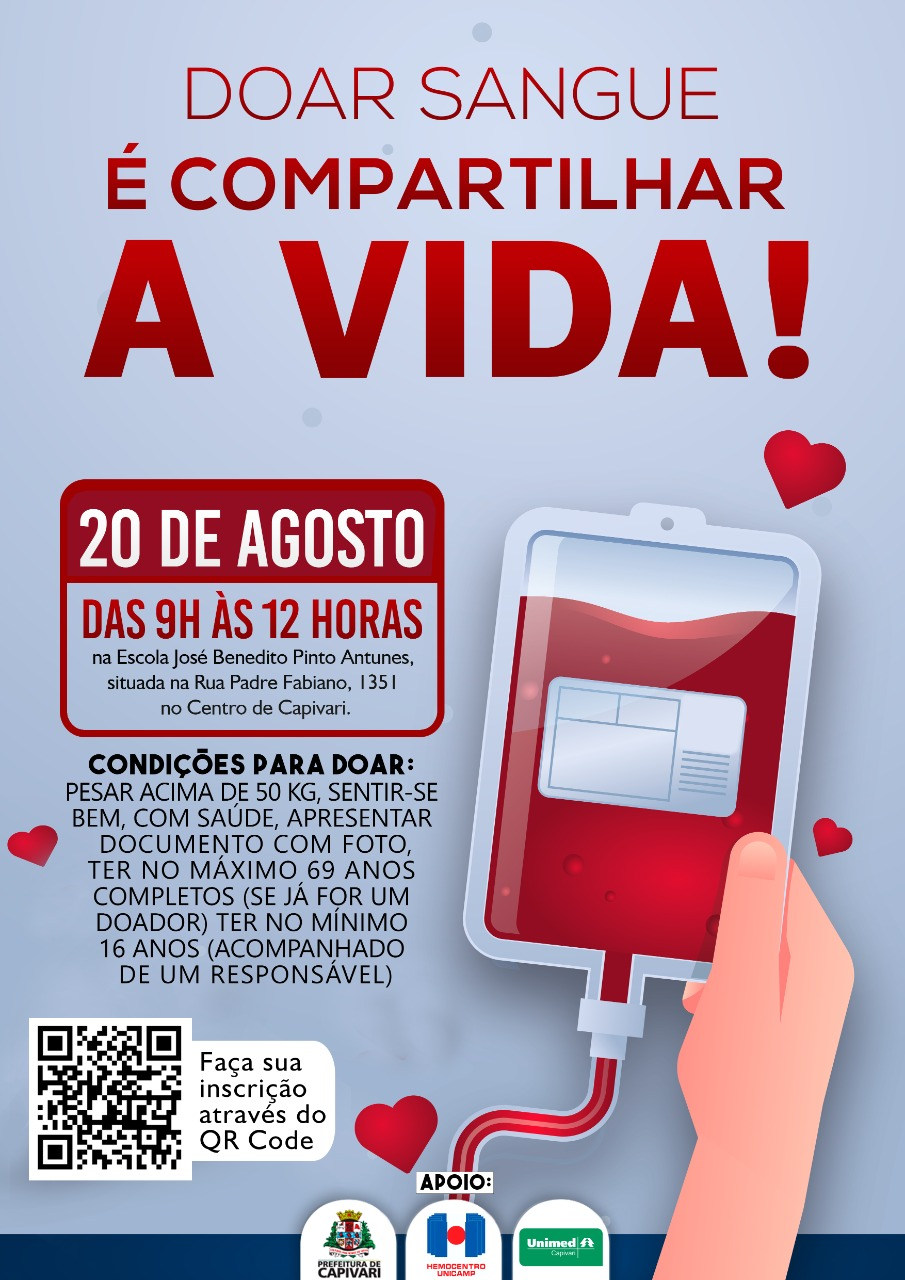
\includegraphics[width=5.76042in,height=8.15278in]{./imgSAEB_7_POR/media/image1.png} \\
\bottomrule
\end{longtable}

\fonte{Prefeitura de Capivari. Secretaria de Saúde anuncia Campanha de Doação de Sangue no dia 20 de agosto. Disponível em:
https://capivari.sp.gov.br/portal/secretaria-de-saude-anuncia-campanha-de-doacao-de-sangue-no-dia-20-de-agosto/
Acesso em: 19 mai. 2023.}

\num{1} A imagem acima representa uma campanha de conscientização. Sabendo que se trata de um texto informativo que tem como objetivo sensibilizar o público, aponte quais os recursos não verbais contribuem para a persuasão.

\linhas{4}
\coment{O uso da imagem da bolsa de sangue sendo segurada como um celular
complementa a escolha da palavra ``compartilhar'' como recursos de persuasão
e sensibilização.}

\num{2} Encontre no texto o verbo que indica uma recomendação de mudança de atitude.
Escreva-o abaixo

\linhas{2}
\coment{Doar, compartilhar. O uso do verbo no infinitivo é uma característica do
gênero. Para incentivar uma atitude, estes tipos de texto utilizam de
linguagem apelativa e multimodal.}

\num{3} Assinale com (V) verdadeiro ou (F) falso as afirmações a seguir sobre os textos
de gênero jornalístico e midiático:

\begin{itemize}

( ) Apresentam linguagem direta

( ) É comum o uso de verbos no imperativo

( ) Servem para divulgar conhecimentos

( ) Tem como objetivo convencer ou informar

\end{itemize}

\coment{V, V, F, V}

Leia o seguinte trecho do Estatuto da Criança e do Adolescente --- ECA.

\begin{quote}
O PRESIDENTE DA REPÚBLICA: Faço saber que o Congresso Nacional decreta e
eu sanciono a seguinte Lei: (\ldots{})

Título II: Dos Direitos Fundamentais (\ldots{})

Capítulo II: Do Direito à Liberdade, ao Respeito e à Dignidade (\ldots{})

Art. 16. O direito à liberdade compreende os seguintes aspectos:

I --- ir, vir e estar nos logradouros públicos e espaços comunitários,
ressalvadas as restrições legais;

II --- opinião e expressão;

III --- crença e culto religioso;

IV --- brincar, praticar esportes e divertir-se;

V --- participar da vida familiar e comunitária, sem discriminação;

VI --- participar da vida política, na forma da lei;

VII --- buscar refúgio, auxílio e orientação. \\

\end{quote}

\fonte{Ministério dos Direitos Humanos e da Cidadania. O Estatuto da Criança e 
do Adolescente -- ECA.
Disponível em: http://www.gov.br/mdh/pt-br/navegue-por-temas/crianca-e-adolescente/publicacoes/o-estatuto-da-crianca-e-do-adolescente. Acesso em: 19 mai. 2023.}

\num{4} Analise a forma composicional do texto e identifique as características que
indicam que ele pertence à esfera jurídica.

\linhas{4}
\coment{As características que indicam que o texto pertence à esfera jurídica são as
seguinte: divisão em artigos e capítulos, uso de numerais romanos, uso de
linguagem formal, verbos no infinitivo.}

\num{5} O uso do verbo no infinitivo em textos jurídicos e legais tem uma função. 
Que função é essa?

\linhas{4}
\coment{Os verbos no infinitivo, no caso de textos de regulamentação, indicam
orientação, têm uma função de persuadir, convencer ou convidar a uma
ação ou atitude.}

\num{6} Analise o texto a seguir e responda às questões a respeito dele. 

% Suprimi essa imagem porque ela não tem grande contribuição para o material. Rogério, 19/5/23, 16h21
%\begin{longtable}[]{@{}
%>{\raggedright\arraybackslash}p{(\columnwidth - 0\tabcolsep) * \real{0.9861}}@{}}
%\toprule
%\endhead
%\textbf{Alerta importante para você que é jovem e vai ler esta cartilha}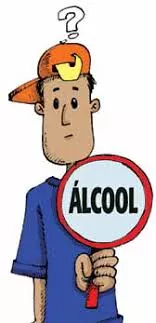
\includegraphics[width=1.625in,height=3.36458in]{./imgSAEB_7_POR/media/image2.png}

\begin{quote}
O Estatuto da Criança e do Adolescente -- ECA -- proíbe a venda de
qualquer tipo de bebida alcoólica para menores de 18 anos.

Portanto, fique esperto!

Se alguém lhe oferecer, mesmo que gratuitamente, qualquer bebida
alcoólica, NÃO ACEITE!

Essa pessoa estará cometendo um crime.

É bom lembrar que o uso do álcool pode levar ao alcoolismo, uma doença
grave que atinge 12,3\% da população brasileira com idade entre 12 e 65
anos.

Entre os jovens de 12 a 17 anos, a taxa de alcoolismo é de 7\%.

Considere que este nível representa 554.000 jovens com sérios problemas
sociais e de saúde.

\end{quote}

\fonte{Portal do Professor do Ministério da Educação. Drogas: Cartilha Álcool e Jovens. 
Disponível em: http://portaldoprofessor.mec.gov.br/storage/materiais/0000011863.pdf.
Acesso em: 2 de abri de 2023.}

\begin{escolha}
  \item A quem se destina este texto? Copie do texto um trecho que justifique
  sua resposta.

\linhas{2}
\coment{O texto se destina a jovens, como se pode verificar por meio do trecho 
``Alerta importante para você que é jovem e vai ler esta cartilha''.}

  \item Releia a frase: ``Considere que este nível representa 554.000 jovens
  com sérios problemas sociais e de saúde.''. Ao utilizar o número que
  representa 7\% da população jovem, o autor traz uma nova informação.
  Qual o sentido de trazer esse número para o texto?

\linhas{4}
\coment{Ao apresentar o número de jovens que sofrem com problemas de alcoolismo, a
informação diz respeito direta e explicitamente ao público-alvo do texto, de modo 
a sensibilizá-lo.}

\end{escolha}

\num{7} No que diz respeito à linguagem, cite duas características comuns aos gêneros
jornalístico e de divulgação científica.

\coment{Tanto no texto jornalístico quanto no de divulgação científica a
linguagem empregada deve ser clara e objetiva e pode haver o uso de
recursos não verbais tais como imagens, gráficos, tabelas.} 

Leia o texto abaixo e responda as questões

\begin{quote}

\emph{Brasília, 23 de março de 2020}

Excelentíssimos(as) senhores(as), Presidente da República, Ministros de
Estado, Governadores(as), Prefeitos(as), Secretários(as) de Saúde e
gestores(as) do SUS,

O CNS, enquanto órgão responsável pelo controle social no SUS, orienta
que todos(as) os(as) referidos(as) nesta carta adotem medidas
emergenciais, em todas as unidades da federação, para os próximos dois
meses (abril e maio), visando conter a crise de Saúde que vivemos hoje e
que pode se agravar nos próximos dias. O objetivo é zelar pela
integridade física e mental dos cidadãos e cidadãs brasileiros, buscando
também ações específicas e sensíveis à realidade de pessoas em regime
carcerário ou cumprindo medidas socioeducativas, dentre outras
populações vulneráveis. (\ldots{})

\emph{Conselho Nacional de Saúde} 

\end{quote} 

\fonte{Conselho Nacional de Saúde. Carta aberta do CNS às autoridades 
brasileiras no enfrentamento ao Novo Coronavírus. Disponível em: https://conselho.saude.gov.br/ultimas-noticias-cns/1074-carta-aberta-do-cns-as-autoridades-brasileiras-no-enfrentamento-ao-novo-coronavirus.
Acesso em: 19 mai. 2023.}

\num{8} A quem se destina a carta?

\linhas{2}
\comente{A carta se destina ao Presidente da República, Ministros de Estado, Governadores (as),
Prefeitos(as), Secretários(as) de Saúde e gestores(as) do SUS.}

\num{9} Selecione do texto um trecho que expressa o motivo de reivindicação da carta.

\linhas{6}
\coment{O trecho que expressa o motivo de reivindicação da carta é ``O CNS, enquanto órgão
responsável pelo controle social no SUS, orienta que todos(as) os(as) referidos(as) nesta
carta adotem medidas emergenciais, em todas as unidades da federação, para os próximos dois
meses (abril e maio), visando conter a crise de Saúde que vivemos hoje e que pode se agravar
nos próximos dias. Nesse sentido, é fundamental que sejam potencializadas ou desenvolvidas as
seguintes ações''. 

\num{10} Relacione os textos e suas características.

% Please add the following required packages to your document preamble:
% \usepackage[table,xcdraw]{xcolor}
% If you use beamer only pass "xcolor=table" option, i.e. \documentclass[xcolor=table]{beamer}
\begin{table}[]
\begin{tabular}{|
>{\columncolor[HTML]{DAE8FC}}l |
>{\columncolor[HTML]{ECF4FF}}c |}
\hline
\textbf{(1) Petição} & (   ) É um texto argumentativo de reivindicação \\ \hline
\textbf{(2) Estatuto} & (   ) Tem como objetivo divulgar informações \\ \hline
\textbf{(3) Folheto} & (   ) Utiliza recursos não verbais como forma de persuasão \\ \hline
\textbf{(4) Notícia} & (   ) Tem por objetivo regulamentar e normatizar \\ \hline
\end{tabular}
\end{table}

\coment{(1) É um texto argumentativo de reivindicação. (4) Tem como objetivo divulgar informações.
(3) utiliza recursos não verbais como forma de persuasão. (2) tem por objetivo regulamentar e
normatizar.}

\colorsec{Treino}

\num{1}

\begin{quote}

De acordo com o professor José Carlos Farah, as quedas em idosos são comuns 
porque o processo de envelhecimento traz algumas perdas importantes no nosso corpo.
A osteopenia, que é a perda de massa óssea, deixa o osso enfraquecido,
e a perda da massa muscular, como consequência, traz a falta do controle
do movimento e equilíbrio, a perda cognitiva, que diminui a nossa
atenção e percepção e a baixa aptidão física''. Ainda segundo o
colunista, o processo de perdas do envelhecimento é inevitável. Mas
alguns hábitos podem ajudar e ele cita entre estes a prática da
atividade física. ``Os benefícios da prática da atividade física se
contrapõem ao processo de envelhecimento. O exercício promove o aumento
da massa muscular e da coordenação motora, do equilíbrio e das funções
cognitivas. Este hábito já diminui a possibilidade de quedas, associado
ao ambiente livre de possíveis obstáculos que podem atrapalhar o dia a
dia do idoso''. 

\end{quote}

\fonte{José Carlos Simon Farah. Jornal da USP. Exercícios físicos podem contribuir 
para a redução da queda de idosos. Disponível em: https://jornal.usp.br/radio-usp/exercicios-fisicos-podem-contribuir-para-a-reducao-da-queda-de-idosos/.
Acesso em: 3 abr. 2023. com adaptações.}

Pode-se afirmar que o trecho acima pertence a um texto de divulgação científica, pois contém:

\begin{escolha}
  
  \item informações técnicas voltadas ao público especializado da área médica.
  
  \item explicações de especialista sobre os benefícios do exercício físico para idosos.
  
  \item citações diretas de artigos científicos sobre benefícios do exercício físico.
  
  \item narrativas pessoais sobre osteopenia em idosos e benefícios do exercício físico..

\end{escolha}

\coment{SAEB: Identificar elementos constitutivos de gêneros de divulgação
científica.

BNCC: EF69LP02 -- Analisar e comparar peças publicitárias variadas
(cartazes, folhetos, outdoor, anúncios e propagandas em diferentes
mídias, spots, jingle, vídeos etc.), de forma a perceber a articulação
entre elas em campanhas, as especificidades das várias semioses e
mídias, a adequação dessas peças ao público-alvo, aos objetivos do
anunciante e/ou da campanha e à construção composicional e estilo dos
gêneros em questão, como forma de ampliar suas possibilidades de
compreensão (e produção) de textos pertencentes a esses gêneros.

a) Incorreta. Embora o texto contenha alguns vocábulos ligados à área médica, não se pode 
afirmar que as informações veiculadas sejam voltadas apenas ao público especializado.
b) Correta. O texto contém explicações sobre os benefícios do exercício físico para idosos.
c) Incorreta. O texto não contém citações de artigos científicos. Há apenas falas curtas de um
especialista no assunto.
d) Incorreta. O texto não contém narrativas pessoais sobre os processos inerentes ao envelhecimento.}

\num{2}

Analise os dois textos a seguir.

\begin{quote}

\textbf{TEXTO 1: ES registra aumento de casos de dengue na 1ª semana de janeiro}

\textit{Em todo o mês de janeiro de 2022, o Espírito Santo teve 951
casos. Só nesta primeira semana já foram 1.453. Infectologista acredita
que estado pode estar vivendo uma epidemia de casos da doença.}

Só na primeira semana do ano foram registrados 1.453 casos da dengue no
Espírito Santo. Número bem maior do que os registros do mês de janeiro
de 2022, quando no mês todo foram registrados 951 casos da doença.

Segundo o infectologista Crispim Cerutti, o estado pode estar vivendo
uma epidemia da doença.

``A gente tem epidemias que ocorrem a aproximadamente a cada três anos. A
última que a gente teve foi em 2019/2020. Embora o intervalo seja um
pouco curto, a gente pode dizer que sim, estamos em uma nova epidemia da
doença. A frequência de casos acompanha o ciclo de vida dos mosquitos'',
explicou o infectologista.

\end{quote}

\fonte{Naiara Arpini. G1. ES registra aumento de casos de dengue na 1ª semana de janeiro.
Disponível em: https://g1.globo.com/es/espirito-santo/noticia/2023/01/18/es-registra-aumento-de-casos-de-dengue-na-1a-semana-de-janeiro.ghtml. Acesso em:
19 mai. 2023.}

\textbf{Exemplo 2: Como eu posso ajudar?}

Para evitar a reprodução do Aedes aegypti, o Ministério da Saúde reúne
uma série de orientações à população. Confira abaixo:

\begin{itemize}
  
  \item Utilize telas de proteção com buracos de, no máximo, 1,5 milímetros nas
janelas de casa;
  
  \item Deixe as portas e janelas fechadas, principalmente nos períodos do nascer e do pôr do sol;
  
  \item Mantenha o terreno limpo e livre de materiais ou entulhos que possam ser criadouros;
  
  \item Tampe os tonéis e caixas d'água;
  
  \item Mantenha as calhas limpas;
  
  \item Deixe garrafas sempre viradas com a boca para baixo;
  
  \item Mantenha lixeiras bem tampadas;
  
  \item Deixe ralos limpos e com aplicação de tela;
  
  \item Limpe semanalmente ou preencha pratos de vasos de plantas com areia;
  
  \item Limpe com escova ou bucha os potes de água para animais;
  
  \item Limpe todos os acessórios de decoração que ficam fora de casa e evite o acúmulo de água em pneus e calhas;
  
  \item Coloque repelentes elétricos próximos às janelas -- o uso é contraindicado para pessoas alérgicas;
  
  \item Velas ou difusores de essência de citronela também podem ser usados;
  
  \item Evite produtos de higiene com perfume, pois podem atrair insetos;
  
  \item Retire água acumulada na área de serviço, atrás da máquina de lavar
  roupa.
 
\end{itemize}

\fonte{Helio Carvalho. G1. Sete cidades da região de Campinas vivem situação de alerta para dengue; entenda o que significa.
Disponível em: https://g1.globo.com/sp/campinas-regiao/noticia/2023/01/17/sete-cidades-da-regiao-de-campinas-vivem-situacao-de-alerta-para-dengue-entenda-o-que-significa.ghtml. 
Acesso em: 19 mai. 2023.}

Os dois exemplos foram retirados de veículos de imprensa e tratam de
questões relacionadas à dengue. Quanto às diferenças e semelhanças entre
os dois exemplos, assinale a alternativa correta:

\begin{escolha}

\item Os dois exemplos pretendem informar a população sobre como evitar os casos de dengue.

\item O primeiro apresenta uma notícia, e o segundo traz indicações de ações de prevenção.

\item O primeiro exemplo é um texto de opinião; o segundo, um folheto informativo.

\item O primeiro texto traz dados científicos sobre a dengue e o segundo é um texto instrucional.

\end{escolha}

\voment{SAEB:Analisar a relação temática entre diferentes gêneros jornalísticos.

a) Incorreta. O primeiro exemplo traz uma notícia sobre o número de casos
e segundo exemplo traz indicações de ações para prevenir a
proliferação do mosquito.

b) Correta. O primeiro exemplo é uma
notícia sobre o número de casos de dengue em 2023; o segundo contém
indicações de ações de prevenção e combate à proliferação do
mosquito que transmite a doença.

c) Incorreta. Embora o segundo exemplo possa ser considerado um texto
informativo, o primeiro exemplo não é um texto de opinião.

d) Incorreta. O primeiro exemplo não traz dados científicos e nem possui
linguagem científica e técnica sobre o assunto.}

\num{3}

Leia os trechos extraídos da constituição Brasileira de 1988 e responda
o que se pede:

Trecho 1:

\begin{quote}

\textbf{Trecho 1}

Art. 1.º A República Federativa do Brasil, formada pela união
indissolúvel dos Estados e Municípios e do Distrito Federal,
constitui-se em Estado democrático de direito e tem como fundamentos: (\ldots{})

Art. 3.º Constituem objetivos fundamentais da República Federativa do
Brasil:

IV - promover o bem de todos, sem preconceitos de origem, raça, sexo,
cor, idade e quaisquer outras formas de discriminação.

Art. 4.º A República Federativa do Brasil rege-se nas suas relações
internacionais pelos seguintes princípios:

III - autodeterminação dos povos;

\end{quote}


\begin{quote}
\textbf{Trecho 2}

Art. 215. O Estado garantirá a todos o pleno exercício dos direitos
culturais e acesso às fontes da cultura nacional, e apoiará e
incentivará a valorização e a difusão das manifestações culturais.

§ 1.º O Estado protegerá as manifestações das culturas populares,
indígenas e afrobrasileiras, e das de outros grupos participantes do
processo civilizatório nacional. Art. 216. Constituem patrimônio
cultural brasileiro os bens de natureza material e imaterial, tomados
individualmente ou em conjunto, portadores de referência à identidade, à
ação, à memória dos diferentes grupos formadores da sociedade
brasileira, nos quais se incluem:

I - as formas de expressão;

II - os modos de criar, fazer e viver;

III - as criações científicas, artísticas e tecnológicas;

IV - as obras, objetos, documentos, edificações e demais espaços
destinados às manifestações artístico-culturais;

V - os conjuntos urbanos e sítios de valor histórico, paisagístico,
artístico, arqueológico, paleontológico, ecológico e científico.

§ 1.º O poder público, com a colaboração da comunidade, promoverá e
protegerá o patrimônio cultural brasileiro, por meio de inventários,
registros, vigilância, tombamento e desapropriação, e de outras formas
de acautelamento e preservação. \\

\end{quote}

\fonte{Constituição da República Federativa do Brasil. Disponível
em: https://www2.senado.leg.br/bdsf/bitstream/handle/id/518231/CF88_Livro_EC91_2016.pdf.
Acesso em: 19 mai. 2023.}

Sobre os trechos selecionados é correto afirmar que:

\begin{escolha}

  \item os dois trechos são contraditórios entre si.

  \item não há relação direta entre os dois trechos.

  \item os dois trechos versam sobre questões distintas.

  \item os dois trechos são complementares. 

\end{escolha}

\coment{SAEB: Identificar formas de organização de textos normativos, legais
e/ou reivindicatórios.

BNCC: EF69LP27 -- Analisar a forma composicional de textos
pertencentes a gêneros normativos/ jurídicos e a gêneros da esfera
política, tais como propostas, programas políticos (posicionamento
quanto a diferentes ações a serem propostas, objetivos, ações previstas
etc.), propaganda política (propostas e sua sustentação, posicionamento
quanto a temas em discussão) e textos reivindicatórios: cartas de
reclamação, petição (proposta, suas justificativas e ações a serem
adotadas) e suas marcas linguísticas, de forma a incrementar a
compreensão de textos pertencentes a esses gêneros e a possibilitar a
produção de textos mais adequados e/ou fundamentados quando isso for
requerido.

a) Incorreta. Os trechos não são contraditórios. O segundo trecho
apenas trata de uma parcela da população em particular enquanto o
primeiro trata do conjunto da população brasileira.

b) Incorreta. Os trechos apresentam relação direta ao passo que a
população indígena faz parte da população brasileira e como tal também
tem direitos civis garantidos pela lei.

c) Incorreta. Os dois trechos versam sobre direitos essenciais, portanto
não tratam de questões distintas.

d)Correta. Os dois trechos apresentam relação de complementaridade, pois
as disposições presentes no segundo trecho apenas especificam direitos
dos povos indígenas e deveres do Estado brasileiro para com essa
população a fim de garantir as obrigações do Estado brasileiro dispostas
no Artigo 3º.}

\chapter{Nas tramas do texto literário}
\markboth{Módulo 3}{}

\colorsec{Habilidades do SAEB}

\begin{itemize}
  
  \item Analisar elementos constitutivos de textos pertencentes ao domínio literário.
  
  \item Analisar a intertextualidade entre textos literários ou entre estes e outros textos 
verbais ou não verbais.
  
  \item Inferir a presença de valores sociais, culturais e humanos em textos literários.

\end{itemize}

\colorsec{Habilidades da BNCC}

\begin{itemize}

  \item EF69LP44, EF69LP47, EF67LP27

\end{itemize}

\conteudo{A literatura, assim como todo o escopo das artes, é uma poderosa
ferramenta de expressão de crenças, valores e ideias de determinada
sociedade. Por meio de textos literários são apreendidos os hábitos, os
acontecimentos, desafios e questões de determinada época. Alguns textos
literários são tão ricos e tratam de temas tão essenciais e universais
que acabam por sobreviver ao tempo. Para além do texto escrito, as
narrativas verbais também servem como meio de eternização de certas
questões, sentimentos e desafios enfrentados pelos seres humanos. Não
por acaso, marcas de intertextualidade permeiam a cultura literária. Em
obras literárias é possível entrever, de forma direta ou indireta, as
relações com outros tipos de arte, verbais e não verbais. A análise dos
elementos constitutivos das produções literárias permite perceber as
características e singularidades para compreender o porquê de algumas
obras serem tão singulares. Elementos tais como enredo e linguagem podem
dizer muito sobre determinados grupos, culturas e épocas. Portanto, a análise dos
aspectos constitutivos dos textos literários e suas narrativas pressupõe
um entendimento da literatura que ultrapassa seu valor estético e dota
de sentido filosófico, sociológico, histórico e antropológico a produção
textual artística. Por isso, é fundamental o estudo de aspectos pertinentes à
linguagem, ao estilo, à estrutura e à temática das narrativas. 
A Literatura tem o poder de despertar sensações,
questionamentos e proporcionar experiências estéticas que se refletem na
maneira como as pessoas escolhem ser e estar no mundo. O reconhecimento
do valor e da importância das obras do domínio literário pode
proporcionar uma formação ética e questionadora que participa da
formação cultural e intelectual da sociedade.}

\coment{Professor(a), questione os estudantes sobre os gêneros textuais
literários que conhecem, retome as principais características
do conto, crônica, poesia, literatura de cordel, romance e demais
gêneros que surgirem.

Reforce a ideia de que tais gêneros retratam a sociedade com seus
valores e desafios. Retome com os os estudantes os conhecimentos
prévios sobre mitos, lendas e demais textos de origem popular e saliente
a forma como os temas trabalhados remontam a hábitos, valores e crenças
da cultura e da época em que foram escritos (lenda do milho, da
mandioca, do arroz, sobre os rios, a paisagem, ritos de passagem,
comemorações, etc). Chame a atenção dos estudantes para o
fato de que os diversos tipos de artes podem se comunicar. Neste caso,
pode ser citado como exemplo o texto dramático --- que
pode ser lido, mas é escrito para ser encenado. Mostre como o teatro
também promove integração de diversas expressões artísticas. Cite também
outras expressões tais como a música e as artes plásticas e estimule os
estudantes a pensarem como essas expressões se complementam.}

\colorsec{Atividades}

\num{1} O conto popular é um gênero literário proveniente da tradição oral e em sua textualidade mantém algumas marcas de estilo quanto à linguagem. Sobre este aspecto da linguagem dos contos populares, cite duas marcas fundamentais deste gênero.

\coment{O gênero conto popular é marcado pela linguagem simples, direta e com
fortes traços de oralidade tais como regionalismos, gírias e expressões
populares.}

\num{2} Textos narrativos curtos e objetivos, baseados em eventos do cotidiano: este gênero textual tem como objetivo divertir, entreter, provocar reflexão ou fazer uma crítica. Qual gênero literário possui essas características?

\coment{As características apresentadas se referem à crônica, que traz questões 
cotidianas e pode conter traços de humor.}

Leia o trecho a seguir e responda as questões:

\begin{verse}

Disse Pedro isso é blasfêmia \\

É bastante astucioso \\

Pistoleiro e cangaceiro \\ 

Esse povo é impiedoso \\

Não ganharão o perdão \\

Do santo Pai Poderoso 


Inda mais tem sua má fama \\

Vez por outra comentada \\

Quando há um julgamento \\

Duma alma tão penada \\

Porque fora violenta \\

Em sua vida é baseada. 

\end{verse}

\fonte{Guaipuan Vieira. A chegada de lampião no céu. Disponível em: http://www.dominiopublico.gov.br/download/texto/rd000001.pdf.
Acesso em: 20 mai. 2023.}

\num{3} O texto acima pertence a qual gênero textual?

\linhas{1}
\coment{O texto pertence à Literatura de Cordel.}

\num{4} Cite duas características do gênero presentes no trecho.

\linhas{4}
\coment{Divisão em estrofes e versos, rima, métrica, temas da cultura
nordestina, no caso o personagem Lampião, marcas de oralidade.}

\num{5} Use a legenda para indicar as características da crônica e do conto.
Marque (1) para o crônica e (2) para o conto. Os dois podem ter
características em comum:

% Please add the following required packages to your document preamble:
% \usepackage[table,xcdraw]{xcolor}
% If you use beamer only pass "xcolor=table" option, i.e. \documentclass[xcolor=table]{beamer}
\begin{table}[]
\begin{tabular}{|
>{\columncolor[HTML]{DAE8FC}}l |l|}
\hline
 & Poucos personagens \\ \hline
 & Curto e objetivo \\ \hline
 & Histórias narram fatos do cotidiano e podem estimular a reflexão \\ \hline
 & Podem surgir de narrativas populares transmitidos pela tradição oral \\ \hline
 & É comum que seja publicado em jornais \\ \hline
\end{tabular}
\end{table}

\coment{
% Please add the following required packages to your document preamble:
% \usepackage[table,xcdraw]{xcolor}
% If you use beamer only pass "xcolor=table" option, i.e. \documentclass[xcolor=table]{beamer}
\begin{table}[]
\begin{tabular}{|
>{\columncolor[HTML]{DAE8FC}}c |l|}
\hline
1, 2 & Poucos personagens \\ \hline
1, 2 & Curto e objetivo \\ \hline
1 & Histórias narram fatos do cotidiano e podem estimular a reflexão \\ \hline
2 & Podem surgir de narrativas populares transmitidos pela tradição oral \\ \hline
1 & É comum que seja publicado em jornais \\ \hline
\end{tabular}
\end{table}
}

Leia o trecho a seguir e responda.

\begin{quote}

Houve noutro tempo um rei que tinha o hábito de jogar, e todos com
quem jogava perdiam. Uma vez convidou a um outro rei para jogar, e, no
dia marcado, este se apresentou; mas perdeu todas as mãos do jogo, até
que se desenganou e despediu-se para se ir embora.

\end{quote}

\fonte{Sílvio Romero. Contos Populares do Brasil. Coleção acervo brasileiro.
Volume 3, 2ª edição. Jundiaí: Cadernos do mundo inteiro, 2018 p. 128.}

\num{6} O que a expressão ``Houve noutro tempo'' quer dizer? Comumente outra
expressão é usada para iniciar os contos. Que expressão é essa?

\linhas{3}
\coment{A expressão faz alusão a um tempo passado indeterminado. Nos contos é
comum que apareça a expressão ``Era uma vez'' com o mesmo significado de
tempo indeterminado.}

\num{7} Com base no trecho acima, indique qual o tipo de narrador.

\linhas{3}
\coment{Com base no trecho, podemos dizer que o tipo de narrador é o
narrador observador.}

\num{8} Sobre a intertextualidade presente nas artes em geral, e em específico
na literatura, assinale verdadeiro (V) ou falso (F) para as seguintes
afirmações.

% Please add the following required packages to your document preamble:
% \usepackage[table,xcdraw]{xcolor}
% If you use beamer only pass "xcolor=table" option, i.e. \documentclass[xcolor=table]{beamer}
\begin{table}[]
\begin{tabular}{|
>{\columncolor[HTML]{DAE8FC}}c |l|}
\hline
 & É a prática de copiar trechos de outras obras \\ \hline
 & \begin{tabular}[c]{@{}l@{}}É um recurso que pode trazer ainda mais possibilidades de\\ interpretação para um texto\end{tabular} \\ \hline
 & \begin{tabular}[c]{@{}l@{}}Pode estar implícita ou explícita em textos e demais obras\\ artísticas\end{tabular} \\ \hline
 & Pode estar presente em traduções, paródias e releituras de obras \\ \hline
 & Pode ser caracterizada como plágio \\ \hline
\end{tabular}
\end{table}

\coment{F, V, V, V, F}

\num{9} No trecho abaixo vemos um exemplo de discurso indireto:

\begin{quote}

O pai explicou: 
--- Filha, você precisa fazer sua tarefa agora. Mais tarde
temos compromisso.

\end{quote}

Passe a frase para o discurso indireto.

\coment{O pai explicou para a filha que ela precisava fazer a tarefa naquele
momento, pois, mais tarde, eles tinham compromisso.}

\colorsec{Treino}

\num{1}

\begin{quote}

\textbf{Lenda da Mandioca}

\emph{Lenda Indígena}

Era uma vez uma índia chamada Atiolô. Quando o chão começou a ficar
coberto de frutinhas de murici, ela se casou com Zatiamarê. As frutinhas
desapareceram, as águas do rio subiram apodrecendo o chão. Depois, o sol
queimou a terra, um ventinho molhado começou a chegar do alto da serra.
Quando os muricis começaram outra vez a cair, numa chuvinha amarela,
Atiolô começou a rir sozinha. Estava esperando uma menininha.

\end{quote}

\fonte{Ana Rosa Abreu e outros autores. Contos tradicionais, fábulas,
lendas e mitos. Disponível em http://www.dominiopublico.gov.br/download/texto/me001614.pdf. Acesso em: 20 mai. 2023)}

Nesse trecho da lenda da mandioca, notam-se traços da cultura
indígena com relação ao modo de explicar a origem dos alimentos, a
origem da natureza, a preservação dos costumes e a contagem do tempo.
Pode-se notar que a fruta murici é indicadora da passagem de certo 
período de tempo. Assinale a alternativa que explica corretamente 
quanto tempo se passou.

\begin{escolha}

  \item É possível inferir que cerca de um ano se passou.
  
  \item Não se pode saber ao certo quanto tempo se passou.
  
  \item A mudança de estação indica a passagem de três meses.  
  
  \item É legítimo pressupor que muitos anos se passaram. 

\end{escolha}

\coment{SAEB: Inferir a presença de valores sociais, culturais e humanos em
textos literários.

BNCC: EF69LP44 -- Inferir a presença de valores sociais,
culturais e humanos e de diferentes visões de mundo, em textos
literários, reconhecendo nesses textos formas de estabelecer múltiplos
olhares sobre as identidades, sociedades e culturas e considerando a
autoria e o contexto social e histórico de sua produção.

a) Correta. O trecho faz alusão à passagem das quatro estações do ano
exemplificadas pelo ciclo natural da fruta murici, além de referir-se
a períodos de seca e cheia, que permitem inferir a passagem de cerca de um ano.
b) Incorreta. Por meio das características citadas, tais como ocorrência
de chuvas e seca, pode-se inferir que um ano se passou.
c) Incorreta. O trecho faz alusão a diversas características das estações
do ano, portanto mais de uma estação se passou, indicando a passagem
de um ano.
d) Incorreta. O trecho faz alusão à passagem das quatro estações do ano
exemplificadas pelo ciclo natural da fruta murici, além de referir-se
a períodos de seca e cheia, que permitem inferir a passagem de cerca de um ano.}

\num{2}

Leia os poemas abaixo e responda:

\textbf{Texto I: Canção do exílio}

\emph{Gonçalves Dias}

\begin{verse}

Minha terra tem palmeiras, \\

Onde canta o Sabiá; \\

As aves, que aqui gorjeiam, \\

Não gorjeiam como lá. 


Nosso céu tem mais estrelas,\\

Nossas várzeas têm mais flores, \\

Nossos bosques têm mais vida, \\

Nossa vida mais amores.


Em cismar, sozinho, à noite, \\

Mais prazer eu encontro lá; \\

Minha terra tem palmeiras, \\

Onde canta o Sabiá. \\


Minha terra tem primores, \\

Que tais não encontro eu cá; \\

Em cismar -- sozinho, à noite -- \\

Mais prazer eu encontro lá; \\

Minha terra tem palmeiras, \\

Onde canta o Sabiá. 


Não permita Deus que eu morra, \\

Sem que eu volte para lá; \\

Sem que desfrute os primores \\

Que não encontro por cá; \\

Sem qu'inda aviste as palmeiras, \\

Onde canta o Sabiá.

\end{verse}

\end{quote}

\fonte{Gonçalves Dias. Primeiros Cantos. Disponível em:
http://www.dominiopublico.gov.br/download/texto/bn000100.pdf.
Acesso em: 6 abr de 2023.}



\begin{quote}

\textbf{Texto II: Canção do exílio}

\emph{Murilo Mendes}

\begin{verse}

Minha terra tem macieiras da Califórnia \\

onde cantam gaturamos de Veneza. \\

Os poetas da minha terra \\

são pretos que vivem em torres de ametista, \\

os sargentos do exército são monistas, cubistas, \\

os filósofos são polacos vendendo a prestações. {[} \ldots{} {]} \\

Ai quem me dera chupar uma carambola de verdade \\

e ouvir um sabiá com certidão de idade!

\end{verse}

\end{quote}

\fonte{Murilo Mendes. Poesias. Rio de Janeiro: José Olympio, 1959.}

A primeira versão, escrita por Gonçalves Dias em 1847, tornou-se
importante obra representante do romantismo. Posteriormente, em 1930, o
poeta modernista Murilo Mendes retomou a poesia de Gonçalves Dias e
criticou as influências estrangeiras na cultura brasileira
apropriando-se do nacionalismo do Romantismo, transpondo-o para o
nacionalismo modernista. Sobre esta relação de
intertextualidade em obras literárias assinale a alternativa correta.

\begin{escolha}

  \item O poema de Murilo Mendes é um plágio do poema de Gonçalves Dias.

  \item O poema de Murilo Mendes não se refere ao poema de Gonçalves Dias.

  \item O poema de Murilo Mendes é uma paródia do poema de Gonçalves Dias.

  \item O poema de Gonçalves Dias é uma paródia do poema de Murilo Mendes.

\end{escolha}

\coment{SAEB: Analisar a intertextualidade entre textos literários ou entre
estes e outros textos verbais ou não verbais.

BNCC: EF67LP27 -- Analisar, entre os textos literários e entreestes e outras manifestações artísticas (como cinema, teatro, música,
artes visuais e midiáticas), referências explícitas ou implícitas a
outros textos, quanto aos temas, personagens e recursos literários e
semióticos

a) Incorreta. Os traços de intertextualidade não se configuram como plágio.
b) Incorreta. Além do título, existem diversas alusões de Murilo Mendes ao 
poema de Gonçalves Dias.
c) Correta. O tipo de intertextualidade entre os dois poemas é chamado de
paródia, que pode satirizar, de criticar ou de homenagear o texto de referência.
Neste caso, Murilo Mendes critica o nacionalismo no Romantismo
brasileiro e junto ao movimento modernista propõe uma nova forma de
nacionalismo que valoriza a cultura brasileira.
d)  O poema de Gonçalves Dias foi escrito cerca de 100 anos antes,
portanto não pode ser baseado no poema de Murilo Mendes.}

\num{3}


\includegraphics[width=4.11458in,height=2.80208in]{./imgSAEB_7_POR/media/image3.png}

\fonte{OBRANOME. Catálogo. Caixa Econômica Federal e
Embaixada da Espanha, no Conjunto Cultural da Caixa, Brasília 2003.}

O poema acima pode ser caracterizado como um poema visual. Os poemas
visuais foram amplamente explorados pelos poetas do concretismo e contêm características próprias. Sobre as características da poesia
concreta, assinale a alternativa correta.

\begin{escolha}

  \item A combinação de palavras e imagens é irrelevante para a criação dos sentidos do poema. 

  \item Regras rígidas para a estrutura em versos rimados e estrofes 
  caracterizam a poesia visual.

  \item Imagens ilustrativas não têm relação com os sentidos propostos 
  pelo autor.

  \item A disposição de letras e palavras na página é recurso de produção de sentidos do poema.

\end{escolha}

\coment{SAEB: Analisar elementos constitutivos de textos pertencentes ao domínio
literário.

a) Incorreta. Na poesia concreta, pode haver combinação de palavras e imagens 
para a criação dos sentidos do poema.
b) Incorreta. Não se verificam versos rimados e estrofes tradicionais na poesia
visual. 
c) Incorreta. As imagens podem fazer parte da constituição do poema e contribuir
para a produção de sentido.
d) Correta. A disposição de letras e palavras na página é, de fato, recurso de
produção de sentidos do poema.}

\chapter{Formas de composição do sentido}
\markboth{Módulo 4}{}

\colorsec{Habilidades do SAEB}

\begin{itemize}
  
  \item Analisar efeitos de sentido produzido pelo uso de formas de apropriação 
  textual (paráfrase, citação etc.).
  
  \item Analisar os efeitos de sentido decorrentes dos mecanismos de construção 
  de textos jornalísticos/midiáticos.

\end{itemize}


\colorsec{Habilidades da BNCC}

\begin{itemize}

  \item EF69LP16, EF69LP43.

\end{itemize}

\conteudo{Há muitos elementos utilizados para argumentação em textos.
Por meio da estrutura do texto, da escolha de palavras e de recursos de estilo,
é possível perceber objetivos e intenções do autor. Os textos argumentativos
-- tais como artigos de opinião, editoriais ou discursos -- apresentam em sua
construção elementos que visam convencer de alguma ideia ou expor determinado 
ponto de vista. Para atingir esse objetivo, o autor se vale da coesão e da 
coerência. Com argumentos consistentes, bem concatenados e ideias claras, 
é possível encaminhar ao leitor as ideias almejadas. Existem recursos adequados
para persuadir ou convencer o
leitor: é o caso de argumentos de especialistas, dados de pesquisas ou exemplos,
entre muitos outros. Toda pessoa que deseja comunicar algo faz uso desses
recursos: no âmbito pessoal, em conversas informais entre colegas e familiares;
no âmbito profissional, em negociações e reuniões; no âmbito político, em
discursos; no âmbito estudantil e acadêmico, na elaboração de teses,
dissertações e apresentações de trabalho. Portanto, saber reconhecer e
utilizar recursos de persuasão e convencimento é fundamental para a 
convivência em sociedade e para a resolução de conflitos nos quais há a
necessidade discursos claros e orientados por argumentos. 

Para cada gênero textual, existem recursos comuns que auxiliam na boa
comunicação, de acordo com a finalidade e intenção do comunicador.
Dentre eles, o uso de aspas para introduzir citações, o uso de exemplos
para produzir argumentos, a escolha das palavras e de expressões de
acordo com o receptor.}

\coment{Professor(a), relembre os estudantes sobre a necessidade de persuasão e
convencimento nos gêneros textuais já estudados. É comum que relacionem
a persuasão aos textos publicitários, mas vá além e discuta recursos de
convencimento também em textos de opinião e em situações cotidianas.}

\colorsec{Atividades}

Leia o texto abaixo para responder as questões:

\begin{quote}

\textbf{Especialistas indicam formas de combate a atos de intimidação}

Um em cada dez estudantes brasileiros é vítima de bullying -- anglicismo
que se refere a atos de intimidação e violência física ou psicológica,
geralmente em ambiente escolar. O dado foi divulgado esta semana pelo
Programa Internacional de Avaliação de Estudantes (Pisa) 2015.

Especialistas, como a professora de psicologia Ciomara Shcneider,
psicanalista de crianças e adolescentes, defendem que pais e escola
devem estar atentos ao comportamento dos jovens e manter sempre abertos
os canais de comunicação com eles. Para ela, o diálogo continua a ser a
melhor arma contra esse tipo de violência, que pode causar efeitos
devastadores em crianças e adolescentes.

A Lei nº 13.185, em vigor desde 2016, classifica o bullying como
intimidação sistemática, quando há violência física ou psicológica em
atos de humilhação ou discriminação. A classificação também inclui
ataques físicos, insultos, ameaças, comentários e apelidos pejorativos,
entre outros.

``Os casos de bullying começam muito mais silenciosos e, por isso, são
mais graves. Quem sofre a agressão não conta nem na escola nem na
família, mas começa a mudar o comportamento'', explica. De acordo com
ela, queda no rendimento escolar, faltas na escola e mudanças no
comportamento são os sinais mais frequentes apresentados por quem sofre
esse tipo de violência. Por isso, família e escola devem estar sempre
atentos para os sinais que são apresentados pelos jovens.

Os mesmos cuidados, alerta a psicóloga, valem para situações enfrentadas
fora da escola, seja no mundo virtual -- como em casos de cyberbullying
--, na vizinhança onde moram ou nos locais que costumam frequentar.

\end{quote}

\fonte{Ministério da Educação. Bullying. Disponível 
em: http://portal.mec.gov.br/component/tags/tag/34487#. 
Acesso em: 20 mai. 2023.}

\num{1} Qual o principal assunto abordado no texto?

\linhas{1}
\coment{O assunto do texto é o bullying.}

\num{2} Cite um elemento do texto que traz maior confiabilidade às informações.

\linhas{3}
\coment{Discursos de autoridade, exemplos, dados de pesquisas e institutos de
pesquisa conferem credibilidade ao conjunto do texto e às informações nele 
contidas.}

\num{3} Qual a função do travessão no primeiro parágrafo do texto?

\linhas{1}
\coment{A função do travessão é explicar o termo bullying.}

\num{4} Transcreva do texto o trecho em que a especialista oferece recursos
para lidar contra esse tipo de violência. 

\linhas{5}
comnet{O trecho solicitado é ``Para ela, o diálogo continua a ser a melhor
arma contra esse tipo de violência, que pode causar efeitos devastadores em
crianças e adolescentes.''}

\num{5} Utilize a legenda para classificar os tipos de argumento selecionados:

% Please add the following required packages to your document preamble:
% \usepackage[table,xcdraw]{xcolor}
% If you use beamer only pass "xcolor=table" option, i.e. \documentclass[xcolor=table]{beamer}
\begin{table}[]
\begin{tabular}{|
>{\columncolor[HTML]{DAE8FC}}l |l|}
\hline
\textbf{(I) Argumento por Provas Concretas} & \begin{tabular}[c]{@{}l@{}}(     ) Especialistas, como a professora de psicologia Ciomara Shcneider,\\ psicanalista de crianças e adolescentes, defendem que pais e escola\\ devem estar atentos ao comportamento dos jovens e manter sempre abertos\\ os canais de comunicação com eles.\end{tabular} \\ \hline
\textbf{(II) Argumento de Autoridade} & \begin{tabular}[c]{@{}l@{}}(     ) Um em cada dez estudantes brasileiros é vítima de bullying -\\ anglicismo que se refere a atos de intimidação e violência física ou\\ psicológica, geralmente em ambiente escolar. O dado foi divulgado esta\\ semana pelo Programa Internacional de Avaliação de Estudantes (Pisa)\\ 2015.\end{tabular} \\ \hline
\textbf{(III) Argumento por Exemplificação} & \begin{tabular}[c]{@{}l@{}}(     ) A Lei nº 13.185, em vigor desde 2016, classifica o bullying como \\ intimidação sistemática, quando há violência física ou psicológica em\\ atos de humilhação ou discriminação. A classificação também inclui\\ ataques físicos, insultos, ameaças, comentários e apelidos pejorativos,\\ entre outros.\end{tabular} \\ \hline
\end{tabular}
\end{table}

\coment{% Please add the following required packages to your document preamble:
% \usepackage[table,xcdraw]{xcolor}
% If you use beamer only pass "xcolor=table" option, i.e. \documentclass[xcolor=table]{beamer}
\begin{table}[]
\begin{tabular}{|
>{\columncolor[HTML]{DAE8FC}}l |l|}
\hline
\textbf{(I) Argumento por Provas Concretas} & \begin{tabular}[c]{@{}l@{}}(II) Especialistas, como a professora de psicologia Ciomara Shcneider,\\ psicanalista de crianças e adolescentes, defendem que pais e escola\\ devem estar atentos ao comportamento dos jovens e manter sempre abertos\\ os canais de comunicação com eles.\end{tabular} \\ \hline
\textbf{(II) Argumento de Autoridade} & \begin{tabular}[c]{@{}l@{}}(I) Um em cada dez estudantes brasileiros é vítima de bullying -\\ anglicismo que se refere a atos de intimidação e violência física ou\\ psicológica, geralmente em ambiente escolar. O dado foi divulgado esta\\ semana pelo Programa Internacional de Avaliação de Estudantes (Pisa)\\ 2015.\end{tabular} \\ \hline
\textbf{(III) Argumento por Exemplificação} & \begin{tabular}[c]{@{}l@{}}(III) A Lei nº 13.185, em vigor desde 2016, classifica o bullying como \\ intimidação sistemática, quando há violência física ou psicológica em\\ atos de humilhação ou discriminação. A classificação também inclui\\ ataques físicos, insultos, ameaças, comentários e apelidos pejorativos,\\ entre outros.\end{tabular} \\ \hline
\end{tabular}
\end{table}
}

\num{6} Copie do texto o trecho em que a especialista explica outro tipo de violência associada ao bullying que ocorre fora da escola

\linhas{5}
\coment{O trecho solicitado é ``Os mesmos cuidados, alerta a psicóloga, valem
para situações enfrentadas fora da escola, seja no mundo virtual -- como em
casos de cyberbullying --, na vizinhança onde moram ou nos locais que costumam frequentar.}

\num{7} Qual o sinal usado para marcar as falas da especialista?

\linhas{1}
\coment{O sinal usado para marcar as falas da especialista são as aspas.}

\num{8} No trecho ``De acordo com ela, queda no rendimento escolar, faltas na
escola e mudanças no comportamento são os sinais mais frequentes
apresentados por quem sofre esse tipo de violência.'' O pronome \textbf{ela} se
refere a quem?

\linhas{1}
\coment{O pronome se refere à professora de psicologia Ciomara Shcneider.}

\num{9} A paráfrase é um recurso muito comum em textos de opinião e
argumentativos. Este recurso visa a reescrita de alguma fala ou
citação sem que seja necessária a referência direta. Retire do texto
um exemplo de paráfrase.

\linhas{4}
O trecho a seguir contém paráfrase: ``Para ela, o diálogo continua a ser a
melhor arma contra esse tipo de violência, que pode causar efeitos devastadores
em crianças e adolescentes.''}

\num{10} Reescreva em forma de paráfrase a seguinte fala da especialista: ``Os 
casos de bullying começam muito mais silenciosos e, por isso, são mais graves. 
Quem sofre a agressão não conta nem na escola nem na família, mas começa a mudar 
o comportamento''

\linhas{6}
\coment{A professora de psicologia explica que por ocorrerem de maneira
silenciosa, os casos de bullying podem ser mais graves. A vítima pode
apresentar mudanças de comportamento e pode não comunicar a escola e a
família sobre as agressões.}

\colorsec{Treino}

\num{1} Leia o texto a seguir para responder à pergunta.

\begin{quote}

\textbf{Como celulares mudaram nossos cérebros}

Como muitos de nós, passo tempo demais no meu celular. E, como muitos de
nós, sou totalmente consciente e costumo me sentir culpada por isso.

Às vezes, deixo o telefone no outro lado da casa ou o desligo, para usar
menos. Mas, no fim, acabo atravessando o corredor mais cedo do que
gostaria de admitir, para fazer algo que só posso fazer com o celular --
ou que ele me permite fazer com mais eficiência.

Há 50 anos, Martin ``Marty'' Cooper fez a primeira chamada de um
telefone móvel. Ele mesmo fabricou o aparelho -- um telefone bege, do
tamanho de um tijolo, muito diferente dos smartphones atuais, que são
finos e revestidos de vidro.

O aparelho de Cooper não tinha câmera e não enviava mensagens de texto.
Hoje, ele não pensa nos smartphones modernos como um aparelho
para fazer chamadas telefônicas.

``Realmente, ele não é um telefone muito bom em muitos aspectos'',
afirma Cooper. ``Pense um pouco. Você pega um pedaço de plástico e
vidro, que é plano, e coloca contra a curvatura da sua cabeça. Sua mão
fica em uma posição desconfortável.''

\end{quote}

\fonte{A Gazeta. Como celulares mudaram nossos cérebros. Disponível em: https://www.agazeta.com.br/hz/viver-bem/como-celulares-mudaram-nossos-cerebros-0423.
Acesso em: 20 mai. 2023.}

Sobre as vozes do texto, assinale a alternativa correta:

\begin{escolha}
  
  \item O texto apresenta a voz do autor e dos usuários de smartphone.
  
  \item O texto apresenta a voz dos criadores e usuários do smartphone.
  
  \item O texto apresenta as vozes do autor e do criador do primeiro telefone móvel.
  
  \item O texto apresenta a voz dos usuários de smartphones e do autor.

\end{escolha}

\coment{SAEB: Analisar efeitos de sentido produzido pelo uso de formas de
apropriação textual (paráfrase, citação etc.).

BNCC: EF69LP43 -- Identificar e utilizar os modos de introdução de
outras vozes no texto -- citação literal e sua formatação e paráfrase
--, as pistas linguísticas responsáveis por introduzir no texto a
posição do autor e dos outros autores citados (``Segundo X; De acordo
com Y; De minha/nossa parte, penso/amos que''...) e os elementos de
normatização (tais como as regras de inclusão e formatação de citações e
paráfrases, de organização de referências bibliográficas) em textos
científicos, desenvolvendo reflexão sobre o modo como a
intertextualidade e a retextualização ocorrem nesses textos.

a)Incorreta. O texto não apresenta a voz dos usuários de smartphones.
b)Incorreta. O texto apresenta as vozes do criador dos usuários de
smartphones. 
c) Correta. O texto apresenta duas vozes: a do autor e a do criador
do primeiro telefone móvel.
d) Incorreta. O texto não apresenta a voz dos usuários de smartphones.}

\num{2} Leia o texto abaixo para responder à pergunta.

\begin{quote}

Os especialistas apontam a vida diante de uma tela como o principal dos
problemas. ``A revolução digital transformou os padrões de movimento das
pessoas e o modo como de se trabalhar, se divertir, aprender e viajar'',
sentencia num artigo, também na \textit{The Lancet}, Mark S. Tremblay,
especialista em vida saudável e obesidade do Instituto de Pesquisas do
Hospital de Ottawa (Canadá).

\end{quote}

\fonte{Patrícia Peiró. El País Brasil. Sedentários e grudados a uma tela. Disponível em:
https://brasil.elpais.com/brasil/2019/11/18/actualidad/1574086350_697117.html.
Acesso em: 21 mai. 2023.}

O uso de aspas no texto acima é indicativo de:

\begin{escolha}

  \item introdução da fala do autor.

  \item destaque para a explicação.

  \item citação de um artigo.

  \item citação da fala de um especialista.

\end{escolha}

\coment{SAEB: Analisar efeitos de sentido produzido pelo uso de formas de
apropriação textual (paráfrase, citação etc.).

BNCC: EF69LP43 -- Identificar e utilizar os modos de introdução de
outras vozes no texto -- citação literal e sua formatação e paráfrase
--, as pistas linguísticas responsáveis por introduzir no texto a
posição do autor e dos outros autores citados (``Segundo X; De acordo
com Y; De minha/nossa parte, penso/amos que''...) e os elementos de
normatização (tais como as regras de inclusão e formatação de citações e
paráfrases, de organização de referências bibliográficas) em textos
científicos, desenvolvendo reflexão sobre o modo como a
intertextualidade e a retextualização ocorrem nesses textos.

a) Incorreta. A voz do autor não pede uso de aspas. 
b) Incorreta. No texto, as aspas não servem para dar destaque e o trecho isolado entre 
elas não é uma explicação.
c) Incorreta. A citação a um artigo não é citada entre aspas.
d) Correta. O trecho entre aspas indica a citação de um especialista em 
vida saudável na revista The Lancet.}

\num{3} Leia a manchete a seguir para responder à pergunta. 

Uso massivo de máscaras pode 'impedir segunda onda de covid-19', diz
estudo.

\fonte{BBC News Brasil. Uso massivo de máscaras pode 'impedir segunda onda de
covid-19', diz estudo. Disponível em: https://www.bbc.com/portuguese/geral-53058930.
Acesso em: 21 mai. 2023.}

Qual dos seguintes elementos da manchete contribui para sensibilizar o leitor 
quanto à necessidade prevenção contra a Covid-19? Assinale a alternativa correta.

\begin{escolha}

  \item O uso massivo de máscaras pela população.

  \item A possibilidade de impedir a segunda onda.

  \item A ameaça de haver uma segunda onda.

  \item A referência a um estudo científico.

\end{escolha}

\coment{SAEB: Analisar os efeitos de sentido decorrentes dos mecanismos de construção
de textos jornalísticos/midiáticos.

a)Incorreta. A necessidade de uso massivo de máscaras não produz o efeito de sentido
solicitado no enunciado. 
b)Correta. A possibilidade de impedir a segunda onda pode sensibilizar o leitor.
c)Incorreta. A segunda onda é apresentada como fato; a possibilidade de
impedi-la é que sensibiliza o leitor.
d)Incorreta. A referência a um estudo confere credibilidade ao texto, mas 
não sensibiliza o leitor quanto à necessidade prevenção contra a Covid-19.}

\chapter{Informações implícitas no texto: fato ou opinião}
\markboth{Módulo 5}{}

\colorsec{Habilidades do SAEB}

\begin{itemize} 

  \item Inferir informações implícitas em distintos textos.

  \item Distinguir fatos de opiniões em textos.

\end{itemize}

\colorsec{Habilidades da BNCC}

\begin{itemize} 

  \item EF67LP04.

\end{itemize} 

\conteudo{Com a rápida expansão da tecnologia digital nas últimas décadas, a
quantidade de informação disponível e acessível está cada vez maior. Em
nenhum outro momento da história, houve tanto acesso a vídeos, imagens,
propagandas, opiniões, artigos acadêmicos, notícias e reportagens,
tutoriais, dentre tantos outros conteúdos. Há que se ter em mente, contudo,
que a crescente quantidade de informações não garante a qualidade dos
conteúdos gerados e distribuídos de maneira vertiginosa pela internet.
Mais do que nunca se faz necessário aprender a distinguir fatos de
opiniões, fontes confiáveis e fontes questionáveis, argumentos sólidos
de opiniões convincentes. Portanto, saber identificar em um texto as
marcas de subjetividade e objetividade, a intertextualidade e
credibilidade das informações apresentadas é muito importante. 
Para isso, é preciso conhecer formas de verificação da informação 
recebida, o suporte conceitual dado a elas, a existência ou não de
evidências, as fontes, e os possíveis interesses por parte daqueles que 
divulgam textos, com argumentos e fatos, ou com opiniões e sugestões. A
habilidade de questionar informações nunca foi tão necessária como é 
nos dias de hoje.}

\coment{Professor(a), chame a atenção dos estudantes para as diferenças entre
opiniões e fatos. Mostre aos alunos como opiniões podem ser convincentes
por apelarem para as percepções e dilemas pessoais. Explique que
opiniões são importantes e tem sua validade, porém não podem ser
transpostas para a construção de um argumento sólido. Mostre como os
fatos são mais convincentes e aponte as formas de construção de
argumentos baseados em fatos e faça as distinções quanto à construção de
argumentos baseados em opiniões. Chame a atenção para a importância
destas distinções para a vida prática.}

\colorsec{Atividades}

\num{1} Leia as afirmações abaixo e assinale (F) para fatos e (O) para
  opiniões na coluna esquerda da tabela. 

% Please add the following required packages to your document preamble:
% \usepackage[table,xcdraw]{xcolor}
% If you use beamer only pass "xcolor=table" option, i.e. \documentclass[xcolor=table]{beamer}
\begin{table}[]
\begin{tabular}{|cc|}
\hline
\multicolumn{2}{|c|}{\cellcolor[HTML]{DAE8FC}\textbf{Fato (F) ou Opinião (O)?}} \\ \hline
\multicolumn{1}{|c|}{}      & A melhor hora para dormir é o começo da tarde     \\ \hline
\multicolumn{1}{|c|}{}      & Dormir 8 horas por dia melhora a saúde            \\ \hline
\multicolumn{1}{|c|}{}      & O médico receitou remédios controlados            \\ \hline
\multicolumn{1}{|c|}{}      & Os remédios controlados são baratos               \\ \hline
\end{tabular}
\end{table}

\coment{O, F, F, O}

\num{2} Descreva algumas diferenças entre fatos e opiniões:

\coment{Fatos podem ser verificáveis de maneira objetiva; opiniões são
subjetivas. Fatos possuem sustentação lógica; opiniões podem ser
sustentadas por impressões e sentimentos. Fatos, geralmente, são
sustentados por fontes seguras, por muitas pessoas que estudam o
assunto; opiniões, por sua vez, se baseiam apenas nas percepções e crenças
do sujeito, e, mesmo que sejam compartilhadas por muitas pessoas, não
podem ser consideradas como conhecimento formal.}

Leia o texto abaixo e responda o que se pede:

\begin{quote}

Após seu lançamento, foi um verdadeiro sucesso. Com um orçamento de
cerca de 103 milhões de dólares, o filme alcançou 457 milhões em todo o
mundo. Já no primeiro fim de semana atingiu 34 milhões e nas duas
primeiras semanas ultrapassou os 100.

\textit{Gladiador} tem muito a oferecer. Não só há a incrível atuação de Russell
Crowe em um dos melhores papéis de sua carreira, ao qual se soma o de
Joaquin Phoenix. O diretor Ridley Scott faz um ótimo trabalho por trás
das câmeras, impulsionadas pela música de Hans Zimmer. O filme contém,
para muitos, algumas das melhores batalhas do cinema e coloca Maximmus
entre os maiores heróis do cinema de ação da década.

\end{quote}

\fonte{Nathalia Jesus. Um dos filmes mais espetaculares e épicos dos anos 2000 que terá uma continuação mais de 20 anos depois. Disponível em: https://www.terra.com.br/diversao/entre-telas/um-dos-filmes-mais-espetaculares-e-epicos-dos-anos-2000-que-tera-uma-continuacao-mais-de-20-anos-depois,f263c91567fd94f7897e1a8812bc8da6j0ywjnl1.html. Acesso em: 21 mai. 2023.}

\num{3} Qual a finalidade do texto?

\linhas{3}
\coment{O texto tem a finalidade de informar sobre o sucesso de bilheteria 
de \textit{Gladiador}, no primeiro parágrafo; no segundo, explicita uma
breve avaliação crítica sobre as atuações e a direção do filme.}

\num{4} Este texto pode ser lido como pertencente a qual gênero textual?

\linhas{2}
\coment{O texto apresenta características de resenha crítica.}

\num{5} O primeiro parágrafo apresenta fatos ou opiniões? Copie do texto um
trecho que justifique sua resposta.

\linhas{3} 
\coment{O primeiro parágrafo apresenta fatos, como se verifica em: ``Já no 
primeiro fim de semana atingiu 34 milhões e nas duas primeiras semanas 
ultrapassou os 100''.}

\num{6} O segundo parágrafo apresenta fatos ou opiniões? Copie um trecho que 
justifique sua resposta

\linhas{3}
\coment{O segundo parágrafo apresenta fatos ou opiniões, como se verifica 
em ``O diretor Ridley Scott faz um ótimo trabalho por trás das
câmeras''.}

\num{7} Quais são os elementos que apoiam a apresentação dos fatos no texto
acima? Cite alguns exemplos. 

\linhas{3}
\coment{A apresentação dos fatos no texto se sustenta por meio de dados
sobre o faturamento do filme, como se observa em: `` Com um orçamento de
cerca de 103 milhões de dólares, o filme alcançou 457 milhões em todo o
mundo.''}

\num{8} Quais são os elementos que qualificam as opiniões? Cite exemplos.

\linhas{3}
\coment{O autor pretende qualificar as opiniões apresentadas por meio do
uso de adjetivos, como se verifica nos trechos destacados em: ``O filme 
contém, para muitos, algumas das \textbf{melhores} batalhas do cinema e 
coloca Maximmus entre os \textbf{maiores} heróis do cinema de ação da 
década.''}

\num{9} Sobre fatos e opiniões, assinale (V) para verdadeiro e (F) 
para falso na coluna esquerda da tabela abaixo.

% Please add the following required packages to your document preamble:
% \usepackage[table,xcdraw]{xcolor}
% If you use beamer only pass "xcolor=table" option, i.e. \documentclass[xcolor=table]{beamer}
\begin{table}[]
\begin{tabular}{|lc|}
\hline
\multicolumn{2}{|c|}{\cellcolor[HTML]{DAE8FC}\textbf{Verdadeiro (V) ou Falso (F)?}} \\ \hline
\multicolumn{1}{|l|}{}     & Fatos são baseados em sentimentos e impressões         \\ \hline
\multicolumn{1}{|l|}{}     & Opiniões são suficientes para adquirir conhecimento    \\ \hline
\multicolumn{1}{|l|}{}     & Opiniões são baseadas em questões objetivas            \\ \hline
\multicolumn{1}{|l|}{}     & Opiniões são baseadas em sentimentos e impressões      \\ \hline
\multicolumn{1}{|l|}{}     & Fatos se apoiam em evidências                          \\ \hline
\end{tabular}
\end{table}

\coment{F, F, F, V, V}

\num{10} Qual o fato implícito no trecho de Dom Casmurro de Machado de Assis apresentado abaixo:

\begin{quote}

``Chega a fazer suspeitar que a mentira é, muita vez, tão involuntária
como a transpiração.''

\end{quote}

\coment{O fato apresentado é que a transpiração é involuntária.}

\colorsec{Treino}

\num{1} Leia o texto abaixo para responder à questão.

\begin{quote}

Em março, o preço da cesta básica caiu em 13 de 17 capitais do país. É
isso o que indica a Pesquisa Nacional da Cesta Básica de Alimentos, cujo
resultado foi divulgado nesta quarta-feira (12/4). O levantamento é
feito mensalmente pelo Departamento Intersindical de Estatística e
Estudos Socioeconômicos (Dieese).

\end{quote}

\fonte{Carlos Rydlewski. Metrópoles. Em março, preço da cesta básica 
cai em 13 de 17 capitais. Disponível em: https://www.metropoles.com/negocios/em-marco-preco-da-cesta-basica-cai-em-13-de-17-capitais.
Acesso em: 21 mai. 2023.}

Sobre o texto acima é correto afirmar que:

\begin{escolha}

  \item emite uma opinião e noticia um fato.

  \item noticia um fato. 

  \item noticia uma opinião apoiada em um fato.

  \item emite opinião. 

\end{escolha}

\coment{SAEB: Distinguir fatos de opiniões em textos.

a) Incorreta. O trecho não contém opinião. 
b) Correta. O texto apresenta dados de pesquisas que comprovam o fato de
que o valor das cestas básicas diminuiu.
c) Incorreta. Apesar de apresentar os dados de pesquisas, o trecho não
contém opinião do autor.
d) Incorreta. O trecho não contém opinião do autor sobre o tema.}

\num{2} Leia o texto abaixo para responder à questão. 

\begin{quote}

Heloisa Oliveira ainda reforça que há muitos desafios a serem ultrapassados para a garantia do investimento na primeira infância. Independentemente das desigualdades sociais, todas as crianças precisam ter assegurados diversos direitos, dentre eles o de brincar.

\end{quote}

\coment{Ana Paula Lisboa. Correio Braziliense. Marco Legal da Primeira Infância comemora cinco anos nesta segunda (8). Disponível em: https://blogs.correiobraziliense.com.br/primeirainfancia/2021/03/07/marco-legal-da-primeira-infancia-comemora-cinco-anos-nesta-segunda-8/
Acesso em: 21 mai. 2023.}

No trecho acima pode-se perceber que as desigualdades sociais pode ser
entendidas como:

\begin{escolha}

  \item uma opinião fundamentada em pesquisa cietífica.
  
  \item parte da opinião de quem profere a afirmação.
  
  \item um fato que dificulta a garantia de direitos.
  
  \item uma opinião embasada em fatos sobre a importância do brincar.

\end{escolha}

\coment{SAEB:Inferir informações implícitas em distintos textos.

BNCC: EF67LP04 -- Distinguir, em segmentos descontínuos de
textos, fato da opinião enunciada em relação a esse mesmo fato.

a) Incorreta. Não há referências no texto às desigualdades sociais como
opinião fundamentada em pesquisa científica.  

b) Incorreta. Na coerência interna do texto, as desigualdades sociais são
apresentadas como fato. 

c) Correto. Na coerência interna do texto, as desigualdades sociais são
apresentadas como fato que dificulta a garantia de direitos.

d) Incorreta. Na coerência interna do texto, as desigualdades sociais são
apresentadas como fato.}

\num{3} Leia o texto abaixo para responder à questão.

\begin{quote}

Barra Torres lembrou que a doença deixou mais de 700 mil famílias de
luto, além de outras pessoas que foram infectadas e ficaram com
sequelas. O diretor presidente da Anvisa ressaltou que o uso de máscaras
protege especialmente as pessoas com sistema imunológico mais suscetível
a doenças, como crianças, grávidas e idosos.  

``Não é razoável que uma celebração (carnaval) como essa à vida, à
alegria, ao relaxamento, depois de tanto tempo de dor e sofrimento e
morte, signifique um risco para todas essas coletividades''.

\end{quote}

\fonte{Basília Rodrigues. CNN Brasil. Presidente da Anvisa defende uso de máscara contra covid-19 e diz que carnaval impõe riscos. Disponível em: https://www.cnnbrasil.com.br/politica/presidente-da-anvisa-defende-uso-de-mascara-contra-covid-19-e-diz-que-carnaval-impoe-riscos/. 
Acesso em: 21 mai. 2023.}

No trecho acima podem ser observadas fatos e opiniões a respeito do uso
de máscaras em aeroportos e rodoviárias durante as festas de carnaval.
Assinale a alternativa correta.

\begin{escolha}

  \item Fato: 700 mil mortos. Opinião: crianças, grávidas e idosos são mais suscetíveis a doenças.

  \item Fato: o carnaval é uma celebração da vida. Opinião: 700 mil pessoas faleceram de covid no país.
  
  \item Fato: os dados de mortos por covid. Opinião: não é razoável que o carnaval signifique risco.
  
  \item Fato: sequelas nos infectados por covid. Opinião: 700 mil pessoas faleceram de covid no país.

\end{escolha}

\coment{SAEB: Distinguir fatos de opiniões em textos.

BNCC: EF67LP04 -- Distinguir, em segmentos descontínuos de textos,
fato da opinião enunciada em relação a esse mesmo fato.

a)Incorreta. É fato que crianças, grávidas e idosos são mais suscetíveis a
doenças. 

b)Incorreta. O entrevistado entende que o carnaval é uma celebração 
da vida, mas essa é apenas sua opinião: outras pessoas podem entender essa
festa popular de outras maneiras. Da mesma maneira, é fato que 700 mil
pessoas perderam a vida por covid no Brasil.  

c) Correta. A matéria apresenta dados sobre os óbitos por covid no
país. Trata-se, portanto, de fatos. No trecho entre aspas, ao afirmar que 
``não é razoável que o carnaval signifique um risco para as coletividades'',
o entrevistado emite sua opinião. 

d) Incorreta. É fato que 700 mil pessoas perderam a vida por covid 
no Brasil.}

\chapter{Humor e as ferramentas da crítica}
\markboth{Módulo 6}{}

\colorsec{Habilidades do SAEB}

\begin{itemize}

  \item Inferir, em textos multissemiótico, efeitos de humor, ironia e/ou
  crítica.

\end{itemize}

\colorsec{Habilidades da BNCC}

\begin{itemize}

  \item EF69LP03, EF69LP05.

\end{itemize}

\conteudo{O que nos faz rir? Existem alguns recursos e maneiras de relacionar
ideias a fim de provocar humor. Muitas vezes, apenas a inversão do
sentido de uma palavra, um trocadilho, uma paródia ou até mesmo um
desenho podem provocar o riso e a reflexão.
Atualmente, os memes representam muito bem a forma como imagens e poucas
palavras podem garantir efeitos de humor, críticas e ironias. Antes dos
memes, associados diretamente ao surgimento da internet, 
charges e tirinhas de jornal já causavam esses efeitos. 

Para que se possa perceber ironia ou crítica em determinado texto, 
é necessário algum conhecimento prévio, ou seja, muitas vezes uma tirinha 
pode se referir a um problema social, a um acontecimento recente ou a alguma
atitude do senso comum. Por isso, tirinhas, charges e memes são recursos
que dialogam com amplos contextos, embora sejam muito simples, diretos e
curtos. Também por esse motivo é comum que charges e tirinhas sejam
publicadas em jornais e revistas digitais, por isso podem ter seu
tempo de validade datado. Os efeitos de sentido presentes nestes 
textos costumam ser o duplo sentido, a ambiguidade, e a ironia. O
duplo sentido é um recurso no qual são utilizadas palavras ou expressões
que possuem diferentes interpretações e significados. A ambiguidade é a
indeterminação de sentido que palavras e expressões carregam e que podem
produzir humor ou expressar ironia por meio das várias interpretações
que uma mesma palavra ou expressão pode ter.}

\coment{Professor(a), estimule os estudantes a pensarem em exemplos. O uso de
memes pode ser bastante motivador pois traz a definição dos termos
estudados para um recurso conhecido pelos estudantes. Estimule-os a
pensar quais são os recursos utilizados e como eles se articulam para
produzir humor ou ironia.}

\colorsec{Atividades}

Leia a tirinha abaixo e responda às questões de 1 a 6.

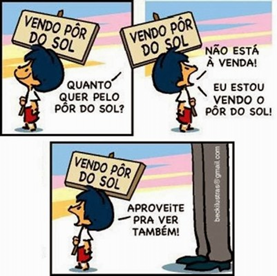
\includegraphics[width=2.88542in,height=2.875in]{./imgSAEB_7_POR/media/image4.png}

\num{1} No meme acima pode-se perceber que o humor está presente. Qual  palavra está sendo usada para produzir esse efeito?

\linhas{1}
\coment{A forma verbal ``vendo'' é utilizada para obter o efeito do 
humor.} 

\num{2} Por que o uso dessa palavra produz efeito de humor?

\linhas{2}
\coment{No contexto, a palavra ``vendo'' pode ter assumir
sentidos diferentes, que causam o efeito de humor.}

\num{3} Quais as possíveis interpretações da palavra usada para produzir
efeito de humor no meme?

\linhas{6}
\coment{A forma verbal ``vendo'' é entendida pela pessoa que faz a pergunta 
como primeira pessoa do singular do presente do indicativo do verbo 
\textit{vender}, isto é: para ele, a criança \textit{está vendendo} o pôr do sol. 
Ela, por sua vez, quer dizer que está 
\textit{observando} o pôr do sol; neste sentido, ``vendo'' é gerúndio do
verbo \textit{ver}.} 

\num{4} Em qual sentido a forma verbal ``vendo'' está sendo usada pela
criança?

\linhas{4}
\coment{A criança quer dizer que está 
\textit{observando} o pôr do sol; neste sentido, ``vendo'' é gerúndio do
verbo \textit{ver}.} 

\num{5} Em qual sentido está sendo compreendida a forma verbal ``vendo''
pela pessoa que faz a pergunta?

\linhas{4}
\coment{A forma verbal ``vendo'' é entendida pela pessoa que faz a 
pergunta como primeira pessoa do singular do presente do indicativo 
do verbo \textit{vender}, isto é: para quem faz a pergunta, a criança 
\textit{está vendendo} o pôr do sol.}

\num{6} Em qual balão a questão das diferentes interpretações da 
forma verbal se esclarece?

\linhas{1}
\coment{As diferentes interpretações da forma verbal se esclarecem 
no último balão.}

Analise a imagem abaixo e responda às questões de 7 a 10. 

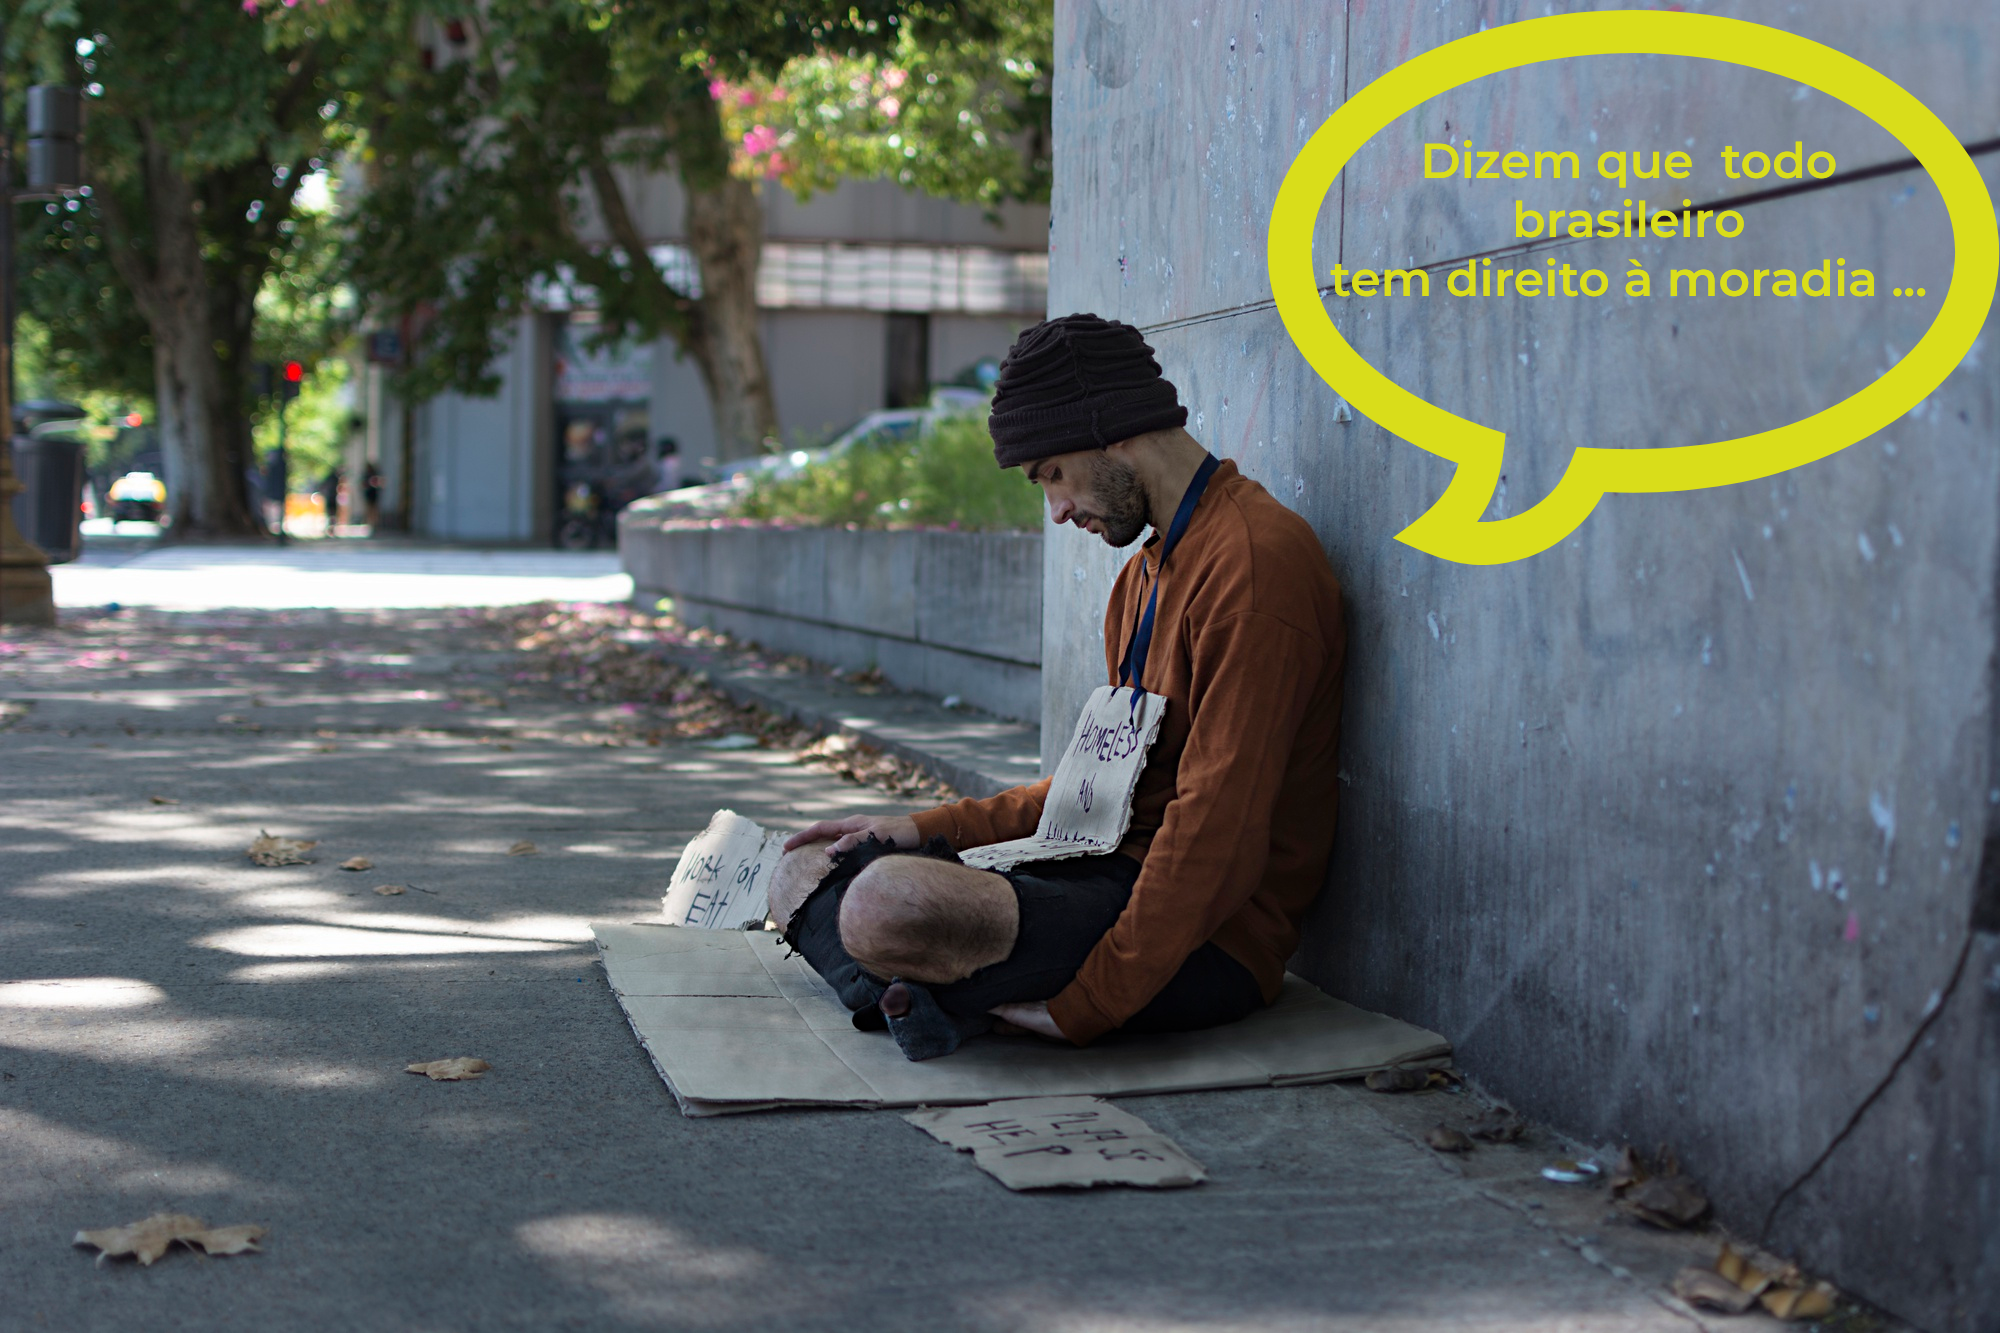
\includegraphics[width=5in,height=3.65625in]{./imgSAEB_7_POR/media/image5.png}

\num{7} Considerando a imagem, é possível
inferir que a fala do morador em situação de rua alude a um importante
documento da democracia brasileira. Que livro é
esse?

\linhas{1}
\coment{É possível inferir que a fala do morador em situação de rua
alude à Constituição Federal de 1988.}

\num{8} Qual a função deste documento e o que ele pretende garantir?

\linhas{5}
\coment{A Constitução Federal trata das questões mais importantes 
para a manutenção da democracia e pretende esclarecer os direitos 
e deveres de todos os âmbitos da sociedade.}

\num{9} Qual o efeito de sentido obtido por meio do meme? 

\linhas{1}
\coment{O efeito de sentido obtido por meio do meme é a ironia.}

\num{10} De que forma a imagem se articula com o texto para produzir
o efeito de sentido?

\linhas{5}
\coment{No meme, uma pessoa em situação de rua reflete sobre um dos direitos 
fundamentais garantidos pela Constituição Federal de 1988: o direito à
moradia. A \textit{declaração} desse direito é rigorosamente oposta à 
\textit{situação concreta} em que se encontra o morador. Essa oposição
compõe a ironia, que consiste em dizer o inverso do que se quer afirmar.
Evidentemente, o autor do meme pretende evidenciar o contraste entre discurso e
prática, isto é, entre a afirmação dos direitos na Constituição de 1988 e a 
desigualdade social.} 

\colorsec{Treino}

\num{1} Leia o trecho abaixo para responder à questão. 

\begin{quote}

Há meio século, os escravos fugiam com frequência. Eram muitos, e nem todos
gostavam da escravidão. Sucedia ocasionalmente apanharem pancada, e nem todos
gostavam de apanhar pancada. Grande parte era apenas repreendida; havia alguém de
casa que servia de padrinho, e o mesmo dono não era mau; além disso, o sentimento da
propriedade moderava a ação, porque dinheiro também dói. A fuga repetia-se,
entretanto. Casos houve, ainda que raros, em que o escravo de contrabando, apenas
comprado no Valongo, deitava a correr, sem conhecer as ruas da cidade.

\end{quote}

\fonte{Machado de Assis. Pai contra Mãe. Disponível em: 
http://www.dominiopublico.gov.br/download/texto/bv000245.pdf.
Acesso em: 22 mai. 2023.}

No fragmento do conto ``Pai contra Mãe'', o narrador de Machado de Assis faz a crítica
à escravidão brasileira por meio de:

\begin{escolha}

  \item repetições que resultam em ironia.
  
  \item relato objetivo da realidade.
  
  \item observações nostálgicas. 
  
  \item valorização dos escravizados. 

\end{escolha}

\coment{SAEB: Inferir, em textos multissemiótico, efeitos de humor, ironia e/ou
crítica.

a) Correta. Nos primeiros períodos do parágrafo, a repetição de 
``nem todos gostavam'', seguida de expressões que se referem à brutalidade
com que os escravizados eram tratados, dirige o olhar do leitor à violência
por eles vivida, naturalizando a linguagem da brutalidade e resultando na 
ironia, por meio da qual Machado de Assis critica a escravidão.
b) Incorreta. Embora haja passagens descritivas da realidade no fragmento, 
a crítica de Machado de Assis só se constitui por meio das ironias no conjunto. 
c) Incorreta. A nostalgia observável em alguns trechos não é suficiente para
estabelecer a crítica, que só terá lugar por meio da naturalização da linguagem
violenta da escravidão. 
d) Incorreta. Não se observa, no texto, a valorização dos escravizados. Evidentemente
Machado de Assis reproduz, no conjunto, a linguagem que os depreciava, evidenciando
a naturalização da brutalidade contra eles.}

\num{2} Observe a imagem abaixo para responder à questão. 

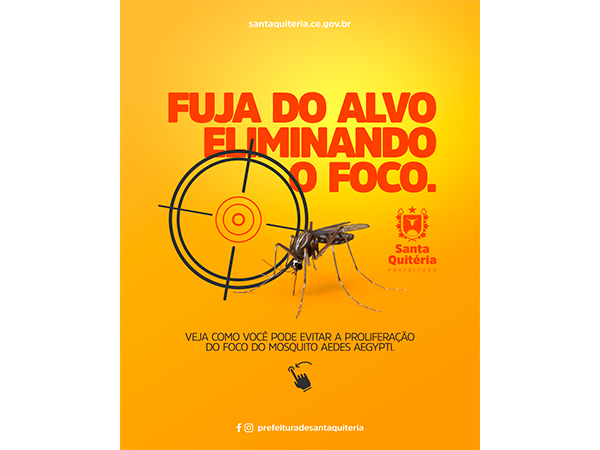
\includegraphics[width=5.90551in,height=4.43056in]{./imgSAEB_7_POR/media/image6.png}

\fonte{Prefeitura de Santa Quitéria. Dicas de como evitar a proliferação 
do foco do mosquito Aedes Aegypti. Disponível em: 
https://www.santaquiteria.ce.gov.br/informa.php?id=1018.
Acesso em: 22 mai. 2023.}

Na imagem acima observa-se uma campanha para evitar a proliferação do
mosquito da dengue. A escolha das palavras e imagens tem como objetivo
sensibilizar a população. Assinale a alternativa que contém as palavras
usadas para a produção de efeito de sentido na campanha. 

\begin{escolha}
  
  \item Proliferação e foco.
  
  \item Veja e evitar.
  
  \item Fuja e elimine.
  
  \item Alvo e foco. 

\end{escolha}

\coment{SAEB: Inferir, em textos multissemiótico, efeitos de humor, ironia e/ou
crítica

BNCC: EF69LP05 -- Inferir e justificar, em textos multissemióticos --
tirinhas, charges, memes, gifs etc. --, o efeito de humor, ironia e/ou
crítica pelo uso ambíguo de palavras, expressões ou imagens ambíguas, de
clichês, de recursos iconográficos, de pontuação etc.

a) Incorreta. A força da campanha é dada pelo jogo entre as palavras
``alvo'' e ``foco''.
b)Incorreta. A força da campanha é dada pelo jogo entre as palavras
``alvo'' e ``foco''.
c)Incorreta. A força da campanha é dada pelo jogo entre as palavras
``alvo'' e ``foco''.
d) Correta. A força da campanha é dada pelo jogo entre as palavras
``alvo'' e ``foco''. De acordo com o texto, deixar de ser alvo do mosquito da
dengue, é preciso eliminar o foco da doença. Além da sonoridade semelhante (ambas
são paroxítonas de duas sílabas terminadas em vogal ``o''), as duas palavras


\num{3}

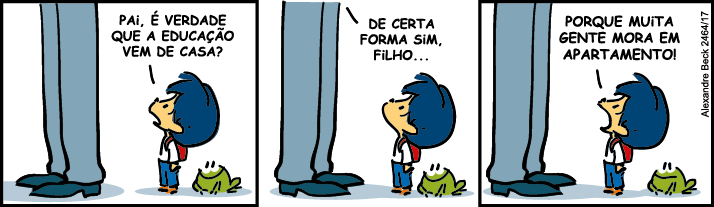
\includegraphics[width=5.90551in,height=1.70833in]{./imgSAEB_7_POR/media/image7.png}

A respeito do meme acima, pode-se afirmar que

\begin{escolha}
    
    \item ironiza a educação por meio do duplo sentido da palavra ``casa''.
    
    \item critica a falta de moradia com o uso da palavra ``casa''.
    
    \item contém propaganda subliminar em benefício da construção de apartamentos.
    
    \item questiona a qualidade de vida dos moradores de apartamentos.

\end{escolha}

\coment{SAEB: Inferir, em textos multissemiótico, efeitos de humor, ironia e/ou
crítica

Bncc: EF69LP05 -- Inferir e justificar, em textos multissemióticos --
tirinhas, charges, memes, gifs etc. --, o efeito de humor, ironia e/ou
crítica pelo uso ambíguo de palavras, expressões ou imagens ambíguas, de
clichês, de recursos iconográficos, de pontuação etc.

a) Correta. No meme, a palavra ``casa'' pode assumir dois sentidos. O primeiro
é figurado: ``casa'' equivale a ``família''; o segundo é literal: a educação
viria da \textit{casa} propriamente dita, que se opõe ao apartamento. A criança 
estaria, assim, ironizando e relativizando, de forma sagaz, a máxima de que 
``a educação vem de casa'' (expressão na qual ``casa'' assume o primeiro dos 
sentidos). Morando em apartamento, o garoto considera o segundo sentido da palavra
``casa'', dispensa a si mesmo da educação e faz a bagunça retratada na imagem.    

b) Incorreta. O meme não contém crítica à falta de moradia.
c) Incorreta. Não há elementos que permitam inferir que o meme contém propaganda 
subliminar. 
d)Incorreta. Não há elementos que permitam inferir que o meme questiona a qualidade 
de vida dos moradores de apartamentos.}

\chapter{Parcialidade nos textos jornalísticos}
\markboth{Módulo 7}{}

\colorsec{Habilidades do SAEB}

\begin{itemize}

  \item Analisar marcas de parcialidade em textos jornalísticos.

  \item Avaliar diferentes graus de parcialidade em textos jornalísticos.

  \item Avaliar a fidedignidade de informações sobre um mesmo fato divulgado 
  em diferentes veículos e mídias.

\end{itemize}

\colorsec{Habilidades da BNCC}

\begin{itemize}

  \item EF07LP02, EF67LP03, EF67LP04.

\end{itemize}

\conteudo{A função ideal do jornalismo é informar de forma imparcial e objetiva
fatos e notícias para oferecer informações e ferramentas para a
formação de opinião. No entanto, nem sempre é possível separar os fatos
das opiniões, pois todo texto, em alguma medida, é produzido a partir
das perspectivas pessoais do autor ou do veículo de comunicação que o
divulga. Por isso, é importante que os leitores aprendam a analisar
marcas de parcialidade em textos jornalísticos, a fim de avaliar o grau
de confiabilidade das informações que estão recebendo.

Uma das formas de identificar as marcas de parcialidade em textos
jornalísticos é perceber o conjunto de valores expressos pelo uso de
adjetivos, advérbios e na forma como são construídos os argumentos nos
textos de divulgação de notícias e acontecimentos. Também a escolha de
fontes e a seleção editorial dos assuntos e temas a serem tratados podem
indicar interesses e, portanto, certo grau de parcialidade. A escolha
dos pontos de vista expressos em uma notícia ou reportagem revela muito
sobre as intenções do autor ou do veículo que divulga o texto. Sendo
assim, comparar fontes e analisar de forma atenta os contextos em que as
informações são divulgadas em cada veículo de informação pode ser uma
forma eficaz de avaliar a confiabilidade e fidedignidade de determinada
notícia ou reportagem, porque a linha editorial e a relação dos
veículos de comunicação com empresas e grupos políticos ou econômicos
podem revelar possíveis interesses e pontos de vista. Portanto, aprender
a avaliar tais marcas de parcialidade e comparar diferentes formas de
divulgação de notícias em diversos veículos e texto é uma habilidade
importante para que o leitor possa formar uma opinião de forma reflexiva
e autônoma.}

\coment{Professor(a), faça um exercício de reflexão com os estudantes,
questionando como percebem os traços e interesses presentes em algumas
manchetes, e chamadas. Chame a atenção para veículos sensacionalistas,
para determinados temas e assuntos abordados e veiculados com a intenção
de gerar polêmicas, discussões ou busca de soluções. Converse com os
estudantes sobre os diversos tipos de textos jornalísticos e estimule-os
a refletir sobre como percebem as marcas de parcialidade. Instrua-os a
pesquisar e questionar os veículos de comunicação trazendo para a
discussão quais podem ser os interesses por trás dos recursos e
elementos multissemióticos presentes nas informações que consomem. Cite
a monetização de determinados conteúdos, explique como é importante
analisar quem são os financiadores e quais as propagandas e empresas
relacionadas aos veículos de informação que conhecem.}

\colorsec{Atividades}

Analise as duas notícias abaixo e responda às questões.

\begin{quote}

\textbf{Texto I}: Cinco desafios para a economia mundial em 2023}

Se 2022 foi um ano difícil para a economia global, 2023 promete ser
ainda pior, com uma recessão a caminho.

Espera-se que 2023 seja o terceiro ano com o pior crescimento econômico
global neste século, atrás de 2009, quando a crise financeira global
causou a Grande Recessão, e 2020, quando os lockdowns da covid-19
virtualmente paralisaram a economia global.

Analistas esperam que as principais economias do mundo, incluindo os
Estados Unidos e o Reino Unido, assim como a zona do euro, entrem em
recessão este ano, já que os bancos centrais continuam aumentando as
taxas de juros para moderar a demanda por bens de consumo e serviços, em
um esforço para conter a inflação. 

\fonte{Ashutosh Pandey. DW. Cinco desafios para a economia mundial em 2023.
Disponível em: https://www.dw.com/pt-br/cinco-desafios-para-a-economia-mundial-em-2023/a-64264182.
Acesso em: 22 mai. 2023. com adaptações.}

\end{quote}

\begin{quote}

\textbf{Texto II}:Por que a inflação mundial deve cair em 2023 (e por que a
notícia não é tão boa)

Provavelmente o pior em termos de inflação já passou.

Pelo menos este é o consenso entre os economistas e as principais
organizações econômicas como o Fundo Monetário Internacional (FMI) ou o
Banco Mundial depois que a maioria dos países do mundo experimentou, em
2022, aumentos de preços não vistos em quatro décadas.

Não há dúvida de que a inflação continuará a pesar no bolso de milhões
de cidadãos em 2023, mas deve registrar uma queda lenta nos próximos 12
meses.

Quando esse período terminar, o FMI espera que a inflação mundial caia
para 4,7\%, pouco menos da metade do nível atual. 

\end{quote}

\fonte{Cristina J. Orgaz. BBC News Brasil. Por que a inflação mundial deve cair em 2023 (e por que a notícia não é tão boa). 
Disponível em: https://www.bbc.com/portuguese/internacional-64145595.
Acesso em: 22 mai. 2023.}

\num{1} Qual é o fato central relatado nas notícias?

\linhas{1}
\coment{O fato central das duas notícias é a crise econômica de 2023.}

\num{2} Quais são as semelhanças entre os fatos noticiados sobre o tema?

\linhas{3}
\coment{As duas notícias tratam da recessão e da influência da queda da
inflação na crise econômica mundial.}

\num{3} Quais são as diferenças entre os fatos noticiados sobre o tema?

\linhas{5}
\coment{No primeiro texto, o autor prevê, em 2023, a continuidade da crise
econômica. O autor segundo sinaliza, por sua vez, uma queda na inflação.} 

\num{4} Em qual das duas notícias a crise mundial é tratada com mais otimismo?
Copie do texto um trecho que justifique sua resposta.

\linhas{3}
\coment{O Texto II é mais otimista, como se verifica no trecho 
``Provavelmente o pior em termos de inflação já passou''.

\num{5} Na tabela abaixo, relacione os títulos numerados à esquerda
com as linhas finas à direita.

  % Please add the following required packages to your document preamble:
% \usepackage[table,xcdraw]{xcolor}
% If you use beamer only pass "xcolor=table" option, i.e. \documentclass[xcolor=table]{beamer}
\begin{table}[]
\begin{tabular}{|ll|lc|}
\hline
\rowcolor[HTML]{CBCEFB} 
\multicolumn{2}{|c|}{\cellcolor[HTML]{CBCEFB}\textbf{Título}} & \multicolumn{2}{c|}{\cellcolor[HTML]{CBCEFB}\textbf{Linha fina}} \\ \hline
\multicolumn{1}{|l|}{(1)} & \cellcolor[HTML]{FFFFFF}Estudiosos alertam para os riscos de doenças cardiovasculares e o sedentarismo & \multicolumn{1}{l|}{(            )} & \cellcolor[HTML]{FFFFFF}\begin{tabular}[c]{@{}c@{}}Análise de hábitos de pacientes com problemas cardiovasculares traz\\ novas informações sobre como prevenir doenças crônicas\end{tabular} \\ \hline
\rowcolor[HTML]{DAE8FC} 
\multicolumn{1}{|l|}{\cellcolor[HTML]{DAE8FC}(2)} & Casos de dengue preocupam secretarias de saúde & \multicolumn{1}{l|}{\cellcolor[HTML]{DAE8FC}(            )} & \begin{tabular}[c]{@{}c@{}}Associação brasileira de pediatria publica estudo sobre os impactos\\ dos jogos e redes sociais na vida de adolescentes\end{tabular} \\ \hline
\multicolumn{1}{|l|}{(3)} & \cellcolor[HTML]{FFFFFF}O perigo está em casa: Pediatras alertam sobre o uso excessivo de telas por crianças e adolescentes & \multicolumn{1}{l|}{(            )} & \cellcolor[HTML]{FFFFFF}\begin{tabular}[c]{@{}c@{}}Ministério da saúde lança cartilha para informar a população sobre\\ as formas de contágio da doença\end{tabular} \\ \hline
\rowcolor[HTML]{DAE8FC} 
\multicolumn{1}{|l|}{\cellcolor[HTML]{DAE8FC}(4)} & Covid-19: Informar para proteger & \multicolumn{1}{l|}{\cellcolor[HTML]{DAE8FC}(            )} & \begin{tabular}[c]{@{}c@{}}Alerta foi dado às secretarias de saúde de todo país, especialmente\\ nas regiões em que se inicia o período de chuvas\end{tabular} \\ \hline
\end{tabular}
\end{table}

\coment{1, 3, 4, 2}

\num{6} Sobre a parcialidade dos textos jornalísticos, assinale V para as
afirmações verdadeiras e F para as afirmações falsas na tabela abaixo.

% Please add the following required packages to your document preamble:
% \usepackage[table,xcdraw]{xcolor}
% If you use beamer only pass "xcolor=table" option, i.e. \documentclass[xcolor=table]{beamer}
\begin{table}[]
\begin{tabular}{|l|l|}
\hline
\rowcolor[HTML]{9698ED} 
\multicolumn{1}{|c|}{\cellcolor[HTML]{9698ED}\textbf{\begin{tabular}[c]{@{}c@{}}Verdadeiro (V) \\ ou \\ Falso (F)\end{tabular}}} & \multicolumn{1}{c|}{\cellcolor[HTML]{9698ED}\textbf{Afirmação}} \\ \hline
 & \begin{tabular}[c]{@{}l@{}}A imparcialidade no jornalismo é importante pois promove a formação\\ de opinião a partir dos fatos apresentados na reportagem\end{tabular} \\ \hline
\rowcolor[HTML]{ECF4FF} 
 & \begin{tabular}[c]{@{}l@{}}O princípio da imparcialidade no jornalismo significa que o\\ jornalista não deve apresentar os diferentes pontos de vista e deixar\\ que o público forme sua própria opinião\end{tabular} \\ \hline
 & \begin{tabular}[c]{@{}l@{}}A imparcialidade no jornalismo pode levar a erros de interpretação e\\ compreensão dos fatos por parte do público, prejudicando a credibilidade\\ da reportagem do jornalista\end{tabular} \\ \hline
\rowcolor[HTML]{ECF4FF} 
 & \begin{tabular}[c]{@{}l@{}}A falta de apresentação de fontes e dados confiáveis pode ser uma\\ característica de parcialidade por parte do jornalista ou do veículo de\\ comunicação colocando em dúvida a credibilidade das notícias veiculadas\end{tabular} \\ \hline
\end{tabular}
\end{table}

\coment{V, F, V, V}

\num{7} Leia os exemplos abaixo e sublinhe as marcas de parcialidade:

\begin{escolha}

  \item Polícia age com violência contra manifestantes pacíficos.

  \item Deputado faz discurso inflamado em defesa dos direitos dos
trabalhadores.

  \item Falas preconceituosas de senadores exibem a impunidade da classe
política no Brasil.

\end{escolha}

\coment{a) Polícia age com \uline{violência} contra manifestantes
\uline{pacíficos}.

b) Deputado faz discurso \uline{inflamado} em defesa dos direitos dos
trabalhadores.

c) Falas \uline{preconceituosas} de senadores exibem a
\uline{impunidade} da classe política no Brasil.}

\num{8} Quais aspectos devem ser levados em conta para questionar a
parcialidade ou imparcialidade de uma notícia

\linhas{8}
\coment{Os aspectos que devem ser levados em conta são: a exposição de
mais de um ponto de vista sobre o mesmo tema, a citação de dados e 
pesquisas de fontes confiáveis e o uso ou não de adjetivos que qualifiquem
os fatos apresentados. É importante também a checagem da veracidade dos 
dados apresentados e o questionamento sobre os contextos em que ocorrem os
fatos e se há interesses políticos ou econômicos por parte do veículo de
comunicação que divulga a notícia.}

\num{9} Analise as duas afirmações a seguir e responda qual das duas apresenta
maior grau de parcialidade. Justifique sua resposta

\begin{itemize}
 
 \item Policiamento nas cidades não gera mais segurança, é o que afirmam
especialistas

  \item Policiamento nas cidades é a principal medida de segurança anunciada pela prefeitura.

\end{itemize}

\linhas{6}
\coment{A primeira afirmação apresenta maior grau de parcialidade, pois
apresenta uma afirmação categórica amparada em afirmação de especialistas. 
A segunda é uma sentença menos parcial, embora contenha o adjetivo ``principal'' para referir-se ao fato noticiado.}

\num{10} De que forma a apresentação de imagens, gráficos e tabelas auxilia 
na formação de opinião de leitores?
\linhas{5}
  
e  a trazer mais credibilidade à notícia, pois podem ser interpretados, 
questionados e verificados.}

\colorsec{Treino}

\num{1} Sabendo da importância de aprender a analisar traços de parcialidade em
textos jornalísticos, assinale a alternativa que contém um recurso por meio
do qual o texto jornalístico tende a ser mais parcial.

\begin{escolha}

  \item Entrevistas com especialistas no assunto abordado.
  \item Diferentes pontos de vista sobre o mesmo assunto.
  \item Adjetivos valorativos para descrever pessoas ou eventos.
  \item Fatos e fontes citadas rigorosamente. 

\end{escolha}

\coment{SAEB: Analisar marcas de parcialidade em textos jornalísticos.

a) Incorreta. Entrevistas com especialistas pretendem obter o efeito da 
imparcialidade.
b) Incorreta. A apresentação de diferentes pontos de vista pretende obter
o efeito da imparcialidade. 
c) Correta. A presença de adjetivos valorativos é marca de parcialidade.
d) Incorreta. A presença de fontes e fatos pretende obter
o efeito da imparcialidade.}

\num{2} Leia o trecho abaixo e o gráfico que segue para responder à questão.

\begin{quote}

Não estamos no caminho certo para atingir as metas de mudança
climática. Se somarmos todas as promessas para reduzir emissões de gases
que provocam efeito estufa pelos países que assinaram o Acordo de Paris,
o mundo ainda esquentaria em mais de 3°C até o fim deste século.

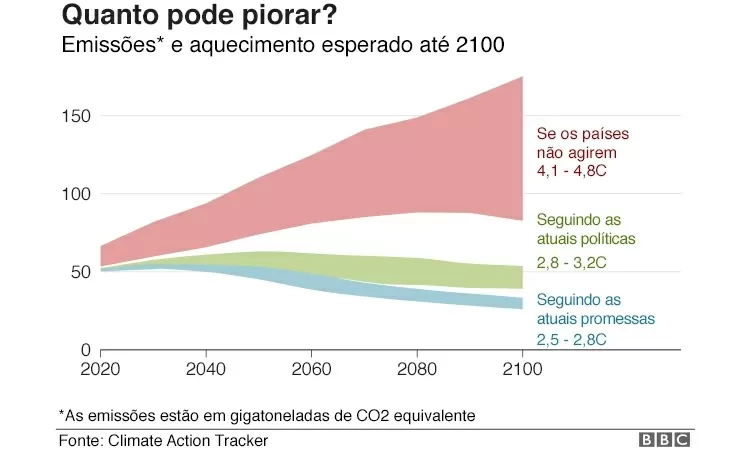
\includegraphics[width=5.90551in,height=3.56944in]{./imgSAEB_7_POR/media/image8.png}

\fonte{BBC News Brasil. Aquecimento global: 7 gráficos que mostram em que ponto estamos. Disponível em: https://www.bbc.com/portuguese/geral-46424720. 
Acesso em: 22 mai. 2023.}

Assinale a alternativa que contém o principal recurso para obter o efeito da 
confiabilidade da notícia:

\begin{escolha}

  \item a opinião do jornalista.
  
  \item a oposição ao Acordo de Paris.
  
  \item o uso de gráficos de pesquisas.
  
  \item o uso de expressões sensibilizadoras.

\end{escolha}

\ciment{SAEB:Avaliar diferentes graus de parcialidade em textos jornalísticos.

BNCC: EF67LP04 -- Distinguir, em segmentos descontínuos de textos,
fato da opinião enunciada em relação a esse mesmo fato.

a) Incorreta. A opinião do jornalista não é um recurso de imparcialidade.
b)Incorreta. O autor não se opõe ao Acordo de Paris, citado como referência às metas
para reversão da situação climática.
c)Correta. O uso de gráficos e recursos similares trazem maior clareza, possibilitando
ao leitor formar suas próprias opiniões
d)Incorreta. O uso de expressões que pretendem sensibilizar o leitor são recursos de
persuasão importantes, mas não conferem imparcialidade ao texto.}

\num{3}

\begin{quote}

\textbf{Após três anos sem reajuste, tarifa de ônibus é corrigida abaixo da
inflação do período}

A partir de 1° de janeiro de 2023, o transporte coletivo urbano de
Joinville passará a operar com os valores de R\$5,25 para a tarifa
antecipada e R\$5,50 para a tarifa embarcada (modalidade utilizada por
apenas 5\% dos passageiros). O reajuste representa aproximadamente
metade do percentual de inflação dos últimos três anos, período no qual
a tarifa não foi corrigida.

\end{quote}

\fonte{Prefeitura de Joinville. Após três anos sem reajuste, tarifa de ônibus é 
corrigida abaixo da inflação do período. Disponível em: https://www.joinville.sc.gov.br/noticias/apos-tres-anos-sem-reajuste-tarifa-de-onibus-e-corrigida-abaixo-da-inflacao-do-periodo/
Acesso em: 22 mai. 2023.}

A matéria apresenta grau de parcialidade, pois apresenta:

\begin{escolha}
  
  \item justificativa para o aumento desde o título.
  
  \item informações precisas sobre a data do ocorrido
  
  \item informações sobre os valores da passagem
  
  \item dados sobre os usuários do transporte público na cidade

\end{escolha}

\coment{SAEB:Analisar marcas de parcialidade em textos jornalísticos.

BNCC: EF67LP04 -- Distinguir, em segmentos descontínuos de textos,
fato da opinião enunciada em relação a esse mesmo fato.

a)Correta. Já no título a notícia apresenta argumentos que levam a crer na
necessidade de reajuste.
b) Incorreta. Essas informações não representam a opinião do veículo e 
podem ser considerados recursos para atribuir veracidade à notícia.
c) Incorreta. Essas informações não representam a opinião do veículo e 
podem ser considerados recursos para atribuir veracidade à notícia.
d) Incorreta. Essas informações não representam a opinião do veículo e 
podem ser considerados recursos para atribuir veracidade à notícia.}

\chapter{Recursos de modalização e argumentação}
\markboth{Módulo 8}{}

\colorsec{Habilidades do SAEB}

\begin{itemize}

  \item Identificar os recursos de modalização em textos diversos.

  \item Analisar os efeitos de sentido dos tempos, modos e/ou vozes 
verbais com base no gênero textual e na intenção comunicativa.

  \item Analisar os efeitos de sentido produzidos pelo uso de modalizadores em textos diversos.

\end{itemize}

\colorsec{Habilidades da BNCC}

\begin{itemize}

  \item EF69LP04, EF69LP28, EF07LP14.

\end{itemize}

\conteudo{A capacidade de identificar e compreender os recursos de modalização
presentes em diferentes tipos de texto é fundamental para uma
comunicação eficiente e coerente. A modalização envolve o uso de
recursos linguísticos para expressar atitudes e opiniões do emissor em
relação ao conteúdo abordado. Esses recursos podem estar
presentes nas formas de uso de modos e vozes verbais, além de adjetivos e advérbios.

A análise dos efeitos de sentido produzidos pelos recursos de
modalização em diferentes gêneros textuais e intenções comunicativas é
fundamental para identificar as influências destes recursos na percepção
e compreensão do conteúdo pelo receptor.

Os recursos de modalização permitem que o emissor expresse suas
opiniões, transmita suas expectativas, faça indicações, influenciando
assim na percepção dos leitores. Dentre os principais recursos
de modalização, encontram-se os tempos verbais, os modos verbais, as
vozes verbais e os modalizadores, que podem reformar graus de
probabilidade, certeza, necessidade e urgência.

Portanto, compreender e utilizar os recursos de modalização de forma
adequada é essencial para produzir textos claros, coerentes e
persuasivos, adaptando a linguagem ao tipo de público alvo e ao contexto
em que são emitidos. Além disso, a análise crítica desses recursos
permite que o leitor compreenda as intenções do emissor e as influências
que podem estar presentes no conteúdo do texto.}

\coment{Professor(a), estimule os estudantes a lembrarem do uso destes recursos
em exemplos conhecidos e práticos tais como campanhas de conscientização
ou publicitárias. Retome os recursos de modalização presentes em
diversos gêneros textuais já estudados demonstrando as diferenças de
interpretação e sentido possíveis para os usos de tempos e modos
verbais, tais como infinitivo e imperativo, das vozes do texto, dos
discursos diretos e indiretos e do uso de advérbios que qualificam as
ações com advérbios que indicam urgência, condições, sugestões,
obrigatoriedade, etc.}

\colorsec{Atividades}


\includegraphics[width=2.85536in,height=2.85536in]{./imgSAEB_7_POR/media/image9.png}

\fonte{https://itajuba.mg.gov.br/secretariaspmi/semdes/nao_desvie_o_olhar/}{\uline{https://itajuba.mg.gov.br/secretariaspmi/semdes/nao\_desvie\_o\_olhar/}}.
Acesso em: 18 de abr de 2023

\num{1} Retire da imagem acima os elementos modalizadores que produzem o sentido de instrução.

\linhas{1}
\coment{As formas verbais no imperativo produzem o sentido de instrução no texto.}

\num{2} De que forma o uso desses recursos sensibiliza o leitor?

\linhas{3}
\coment{As formas verbais no imperativo apelam para a responsabilidade individual do leitor quanto
à violência contra crianças e adolescentes.}

\num{3} Observe as informações contidas no cartaz e explique qual é a ação
recomendada ao tomar conhecimento de casos de violência contra crianças e adolescentes.

\linhas{2}
\coment{Ligar para o telefone indicado e denunciar a violência contra crianças e adolescentes é 
a ação recomendada.}

\num{4} Relacione as colunas de expressões com seus respectivos efeitos de sentido:

% Please add the following required packages to your document preamble:
% \usepackage[table,xcdraw]{xcolor}
% If you use beamer only pass "xcolor=table" option, i.e. \documentclass[xcolor=table]{beamer}
\begin{table}[]
\begin{tabular}{|cc|cc|}
\hline
\rowcolor[HTML]{FD6864} 
\multicolumn{2}{|c|}{\cellcolor[HTML]{FD6864}\textbf{Efeito de sentido}} & \multicolumn{2}{c|}{\cellcolor[HTML]{FD6864}\textbf{Expressão}} \\ \hline
\multicolumn{1}{|c|}{\textbf{I}} & Obrigação & \multicolumn{1}{c|}{} & felizmente \\ \hline
\rowcolor[HTML]{FFCCC9} 
\multicolumn{1}{|c|}{\cellcolor[HTML]{FFCCC9}\textbf{II}} & Apreciação & \multicolumn{1}{c|}{\cellcolor[HTML]{FFCCC9}} & é dever de todos \\ \hline
\multicolumn{1}{|c|}{\textbf{III}} & Possibilidade & \multicolumn{1}{c|}{} & é impossível \\ \hline
\rowcolor[HTML]{FFCCC9} 
\multicolumn{1}{|c|}{\cellcolor[HTML]{FFCCC9}\textbf{IV}} & Certeza & \multicolumn{1}{c|}{\cellcolor[HTML]{FFCCC9}} & provavelmente \\ \hline
\end{tabular}
\end{table}

\coment{II, I, IV, III}

Leia a afirmação abaixo e responda à questão.

\begin{quote}

\textbf{Certamente}, com a implementação dos projetos de mobilidade
urbana, as pessoas passarão a ter mais qualidade de vida e mais
liberdade para explorar e ocupar a cidade.

\end{quote}

\num{5} Qual sentido a palavra destacada pretende expressar?

\linhas{2}
\coment{A palavra destacada pretende expressar certeza sobre as consequências da melhoria da
mobilidade urbana.}

Observe a campanha a seguir e responda:


\includegraphics[width=5.90551in,height=1.47222in]{./imgSAEB_7_POR/media/image10.png}

\fonte{Agência de Transporte do Estado de São Paulo. #FocaNaVida. Disponível em:
http://www.artesp.sp.gov.br/Style\%20Library/extranet/campanha-interna.aspx?id=1
Acesso em: 22 mai. 2023.}

\num{6} Qual a ideia transmitida pela conjunção ``se'' na frase, 
``Nesse carnaval se beber, não dirija''?

\linhas{2}
\coment{A conjunção ``se'', na frase analisada, é condicional, ou seja, é por meio dela que 
se propõe a condição expressa na frase: caso o leitor tenha bebido, não deve dirigit.} 

\num{7} Ainda sobre a campanha acima, assinale verdadeiro ou falso na tabela para as afirmações a seguir.

% Please add the following required packages to your document preamble:
% \usepackage[table,xcdraw]{xcolor}
% If you use beamer only pass "xcolor=table" option, i.e. \documentclass[xcolor=table]{beamer}
\begin{table}[]
\begin{tabular}{|l|c|}
\hline
\rowcolor[HTML]{9AFF99} 
\multicolumn{1}{|c|}{\cellcolor[HTML]{9AFF99}\textbf{\begin{tabular}[c]{@{}c@{}}Verdadeiro (V)\\ ou\\ Falso (F)\end{tabular}}} & \textbf{Afirmação} \\ \hline
 & a campanha sugere que não se deve dirigir após beber \\ \hline
\rowcolor[HTML]{FFFFC7} 
 & a campanha sugere que as pessoas não devem beber durante o carnaval \\ \hline
 & a campanha orienta os foliões a não dirigir no carnaval \\ \hline
\rowcolor[HTML]{FFFFC7} 
 & a campanha pretende alertar sobre a violência no trânsito \\ \hline
\end{tabular}
\end{table}

\coment {V, F, F, F}

\num{8} Leia os enunciados e enumere as proposições na tabela.

% Please add the following required packages to your document preamble:
% \usepackage[table,xcdraw]{xcolor}
% If you use beamer only pass "xcolor=table" option, i.e. \documentclass[xcolor=table]{beamer}
\begin{table}[]
\begin{tabular}{|c|c|c|c|}
\hline
\rowcolor[HTML]{ECF4FF} 
 & Enunciado &  & Efeito \\ \hline
1 & É necessária a presença de um acompanhante &  & Expressa proibição \\ \hline
2 & É proibida a entrada de acompanhante &  & Expressa obrigatoriedade \\ \hline
3 & É permitida a entrada de um acompanhante &  & Expressa permissão \\ \hline
\end{tabular}
\end{table}

\coment{2, 1, 3}

%Leia tirinha abaixo para responder à questão.

%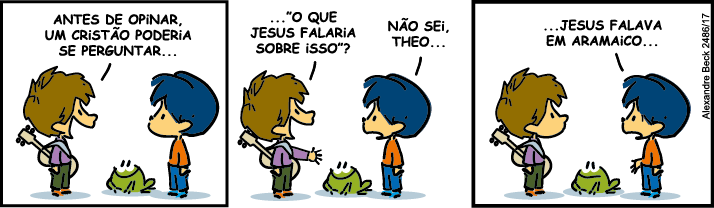
\includegraphics[width=5.90551in,height=1.72222in]{./imgSAEB_7_POR/media/image11.png}

%\fonte{https://tirasarmandinho.tumblr.com/}{\uline{https://tirasarmandinho.tumblr.com/}}
%Acesso em 19 de Abr de 2023

%\num{9}
%Qual é a confusão comunicativa presente na tirinha?
%
%
%A confusão se dá pois os personagens entendem o verbo falar em sentidos diferentes

%\num{10} Qual o sentido do verbo falar no segundo quadrinho? Escreva um sinônimo.

%O verbo falar no segundo quadrinho se refere a opinião, e poderia ser
%substituído por dizer ou pensar. Pensaria, diria.

\colorsec{Treino}

\num{1} Leia o texto abaixo para responder à questão.

\begin{quote}

Antes da pandemia causada pelo novo coronavírus, era quase impensável
ver grande parte da população usando máscaras de proteção na rua.
Contudo a situação mudou, principalmente após o governo do estado tornar
seu uso obrigatório. Mesmo assim, ainda há dúvidas de parte da população
quanto à necessidade e ao benefício do seu uso.

\end{quote}

\fonte{Secretaria de Estado de Saúde de Minas Gerais. Notas de Recomendação: Covid 19.
Disponível em: https://coronavirus.saude.mg.gov.br/blog/101-mascaras-e-covid-19.
Acesso em: 22 mai. 2023.}

No contexto em que se insere, a expressão ``mesmo assim'' expressa oposição entre:


\begin{escolha}

  \item o período anterior e o posterior à pandemia do coronavírus.

  \item a alta adesão da população ao uso de máscaras e a obrigatoriedade de usá-las.

  \item a obrigatoriedade do uso de máscaras e a atitude da população quanto a essa medida.

  \item grande parte da população utilizando máscaras de proteção e a minoria em dúvida.

\end{escolha}

\coment{SAEB: Analisar os efeitos de sentido produzidos pelo uso de modalizadores em textos diversos.

BNCC: EF07LP14 -- Identificar, em textos, os efeitos de sentido do
uso de estratégias de modalização e argumentatividade.

a) Incorreta. No trecho em que se insere, a expressão indicada opõe a afirmação anterior, sobre
a obrigatoriedade do uso de máscaras decretada pelo governo, e a posterior, ``ainda há dúvidas 
de parte da população quanto à necessidade e ao benefício do seu uso''. 
b) Incorreta. No trecho em que se insere, a expressão indicada opõe a afirmação anterior, sobre
a obrigatoriedade do uso de máscaras decretada pelo governo, e a posterior, ``ainda há dúvidas 
de parte da população quanto à necessidade e ao benefício do seu uso''.
c) Correta. No trecho em que se insere, a expressão indicada opõe a afirmação anterior, sobre
a obrigatoriedade do uso de máscaras decretada pelo governo, e a posterior, ``ainda há dúvidas 
de parte da população quanto à necessidade e ao benefício do seu uso''.
c)Incorreta. No trecho em que se insere, a expressão indicada opõe a afirmação anterior, sobre
a obrigatoriedade do uso de máscaras decretada pelo governo, e a posterior, ``ainda há dúvidas 
de parte da população quanto à necessidade e ao benefício do seu uso''.}

\num{2} Leia o texto abaixo para responder à questão. 

\begin{quote}

Carlos observava toda aquela pompa ao seu redor. Ele mesmo estava de passagem,
era um turista simples, brasileiro comum, passeando a custo do dinheiro suado, 
guardado todo mês, para conhecer aquela terra estrangeira e faustosa, cheia de 
gente milionária e bem vestida, cheirosa e fútil. Como deve ser triste depender
do luxo para ser feliz! --- pensava ele.     

\end{quote}

\fonte{Rogério Duarte. Viagens pela terra dos outros. Saíra Editorial. no prelo.}

Na frase ``Como \textbf{deve} ser triste depender do luxo para ser feliz!'', 
a forma verbal destacada expressa:

\begin{escolha}
  
  \item Obrigação
  
  \item Conselho
  
  \item Causa
  
  \item Possibilidade

\end{escolha}

\coment{SAEB:Analisar os efeitos de sentido dos tempos, modos e/ou vozes verbais
com base no gênero textual e na intenção comunicativa.

a) Incorreta. A forma verbal ``deve'', no contexto em que se insere, expressa possibilidade.
b) Incorreta. A forma verbal ``deve'', no contexto em que se insere, expressa possibilidade.
c) Incorreta. A forma verbal ``deve'', no contexto em que se insere, expressa possibilidade.
d) Correta. A forma verbal ``deve'', no contexto em que se insere, expressa possibilidade.}

\num{3}

Analise o cartaz abaixo:


\includegraphics[width=5.90551in,height=4.29167in]{./imgSAEB_7_POR/media/image13.png}

\fonte{Ministério da Integração e do Desenvolvimento Regional. Consumo consciente da água 
é base para um futuro sustentável. Disponível em: https://www.gov.br/dnocs/pt-br/assuntos/noticias/consumo-consciente-da-agua-e-base-para-um-futuro-sustentavel.
Acesso em: 22 mai. 2023.}

O uso do gerúndio na campanha acima expressa:

\begin{escolha}

  \item ação contínua.
  \item ordem a ser acatada.
  \item sugestão a ser considerada.
  \item condição.

\end{escolha}

\coment{SAEB: Analisar os efeitos de sentido dos tempos, modos e/ou vozes
verbais com base no gênero textual e na intenção comunicativa.

BNCC: EF69LP04 -- Identificar e analisar os efeitos de sentido
que fortalecem a persuasão nos textos publicitários, relacionando as
estratégias de persuasão e apelo ao consumo com os recursos
linguístico-discursivos utilizados, como imagens, tempo verbal, jogos de
palavras, figuras de linguagem etc., com vistas a fomentar práticas de
consumo conscientes.

a) Incorreta. No contexto em que se insere, a forma verbal no gerúndio tem valor condicional: 
``Água: se soubermos usar, não vai faltar''. 
b) Incorreta. No contexto em que se insere, a forma verbal no gerúndio tem valor condicional: 
``Água: se soubermos usar, não vai faltar''. 
c) Incorreta. No contexto em que se insere, a forma verbal no gerúndio tem valor condicional: 
``Água: se soubermos usar, não vai faltar''.
d) Incorreta. No contexto em que se insere, a forma verbal no gerúndio tem valor condicional: 
``Água: se soubermos usar, não vai faltar''.}  

\chapter{Figuras de linguagem como estratégia argumentativa}
\markboth{Módulo 9}{}

\colorsec{Habilidades do SAEB}

\begin{itemize}
  
  \item Analisar o uso de figuras de linguagem como estratégia argumentativa.

  \item Avaliar a eficácia das estratégias argumentativas em textos de diferentes gêneros.

\end{itemize}

\colorsec{Habilidades da BNCC}

\begin{itemize}

  \item EF69LP17, EF67LP38.

\end{itemize}

\conteudo{A linguagem tem como principal objetivo a comunicação, portanto, é
impossível distinguir a linguagem da interação que ela provoca. Quanto
maior o domínio das ferramentas de linguagem por parte do autor, maior o
nível de interação e conexão será atingido com o leitor. Do outro lado,
quanto mais o leitor for capaz de reconhecer as ferramentas e recursos
de expressividade, melhor será sua experiência de leitura. Existem diversas 
maneiras de promover maior expressividade
das palavras e, assim, facilitar e potencializar a interação por meio
da comunicação. Dentre esses recursos estão as chamadas figuras de
linguagem. São formas de interação que podem trazer maior expressividade 
ao texto, seja ele escrito ou transmitido oralmente.

Cada figura de linguagem tem características próprias e pode ser
utilizada de diversas maneiras, de acordo com o objetivo do falante ou
do escritor, com a situação comunicativa e com o interlocutor. As
figuras de linguagem podem fazer alusão ao sentido figurado das palavras
e expressões, tratar com exagero para exacerbar características e
impressões ou contrapor palavras com sentidos antagônicos demonstrando
valores de forma implícita. Por essas características, as figuras de
linguagem são recursos comunicativos de grande utilidade, especialmente
para escrita de textos do campo artístico literário como letras de
música e poemas. Também podem apresentar-se como recurso de persuasão e
comunicação importante nos textos do campo jornalístico
midiático.

A \textbf{metáfora} é uma figura de linguagem utilizada para
estabelecer uma relação de semelhança e comparação entre dois termos
distintos. Um exemplo do uso da metáfora é a expressão ``sua vida era um
mar de rosas''. Nesse caso, a expressão ``mar de rosas'' não tem sentido
literal, mas figurado, pois se refere a algo agradável e
prazeroso e não ao mar em sentido literal.

A \textbf{metonímia}, por sua vez, é a figura de linguagem utilizada quando se
lança mão um termo para se referir a outro, com o qual ele mantém uma
relação de proximidade, contiguidade e pertencimento. Ou seja, dizer que
``a cidade se beneficiou com as obras de infraestrutura'' é utilizar a metonímia,
por meio da qual o termo ``a cidade'' se refere à população da cidade. A metonímia
tem o efeito de tornar a linguagem mais concisa e precisa, evitando a repetição de
termos e textos muito extensos. É uma forma de dinamizar a comunicação e
potencializar a capacidade comunicativa.

Por meio da \textbf{personificação} atribuem-se características humanas a animais
e objetos. A personificação tem o efeito de tornar a linguagem mais expressiva e 
poética, pois humaniza seres e fenômenos, produzindo alto grau de identificação do
leitor com a experiência, sensação ou impressão que se pretende comunicar.

Por fim, a \textbf{hipérbole} é a figura de linguagem que aumenta ou exagera
determinada característica como forma de expressão.

\coment{Professor(a) faça um levantamento dos conhecimentos prévios que os 
estudantes já têm. Deixe que tragam
exemplos e forneça mais informações sobre os conceitos, chamando a
atenção para as possibilidades expressivas das figuras de linguagem.
Mostre como o uso das figuras de linguagem podem ampliar os efeitos de
sentido, em quaisquer gêneros textuais.}

\colorsec{Atividades}

Leia os primeiros versos do Hino Nacional Brasileiro para responder às perguntas:

\begin{quote} 

Ouviram do Ipiranga as margens plácidas
De um povo heroico o brado retumbante.

\end{quote}

\fonte{Joaquim Osório Duque Estrada. Hino Nacional Brasileiro. 
Disponível em: https://www.planalto.gov.br/ccivil_03/constituicao/hino.htm.
Acesso em: 22 mai. 2023.}

\num{1} Coloque os versos e termos da oração na ordem direta para compreender 
melhor o sentido da frase. 

\linhas{2}
\coment{As margens plácidas do Ipiranga ouviram o brado retumbante de um povo heroico.}

\num{2} Quais são as figuras de linguagem presentes nos dois primeiros versos do 
Hino Nacional Brasileiro? Justifique sua resposta.

\linhas{5}
\coment{As figuras de linguagem são o hipérbato -- isto é, a inversão dos termos -- e a
personificação, atribuição de ações humanas (ouvir) a seres inanimados (as margens do 
Rio Ipiranga).}

\num{3} Qual é a figura de linguagem presente na frase ``Você tem um coração de pedra!''? 
Explique.

\linhas{5}
\coment{Na frase ``Você tem um coração de pedra!'' existe metáfora. A metáfora é uma comparação
cujos termos são omitidos. Nesse caso, a comparação se dá por meio do elemento comum à pedra
e ao coração: sua \textit{dureza}.}

\num{4} Qual é a figura de linguagem presente na frase  ``Estou morrendo de medo''? Explique.

\linhas{3}
\coment{Na frase  ``Estou morrendo de medo'' observa-se hipérbole, devido ao exagero.}

\num{5} Qual é a figura de linguagem presente na frase  ``As estrelas são os olhos dos deuses''?
Explique.

\linhas{5}
\coment{Na frase ``As estrelas são os olhos dos deuses'' existe metáfora. A metáfora é uma comparação
cujos termos são omitidos. Nesse caso, a comparação se dá por meio do elemento comum às estrelas e 
e aos olhos: seu \textit{brilho e/ou sua posição privilegiada em relação aos homens}.}

\num{6} Sobre a hiperbole, assinale V para as afirmações verdadeiras e F para as falsas:

\begin{table}[]
\begin{tabular}{|c|c|}
\hline
\textbf{\begin{tabular}[c]{@{}c@{}}Verdadeiro (V) \\ ou\\ Falso (F)?\end{tabular}} &  \\ \hline
 & comparação entre palavras distintas, sem mostrar os termos dessa comparação \\ \hline
 & exagero do sentido de uma palavra ou expressão \\ \hline
 & substituição de uma palavra por outra \\ \hline
 & atribuição de características humanas a seres inanimados \\ \hline
\end{tabular}
\end{table}

\coment{F, V, V, F}

Leia o texto abaixo para responder às questões.

\begin{quote}

Na cordilheira que fica em cima do vale de Yyucay, em Cusco,
pode-se ouvir todos os sons. O vento sopra com sua bocarra;
a manhã, obrigada a se levantar sempre antes dos outros,
boceja morta de sono; os pássaros, seus eternos namorados,
acordam cantando ao ouvi-la se espreguiçar.

\end{quote}

\fonte{Ana Rosa Abreu e outros autores. Alfabetização: livro do aluno. Vol.2: 
contos tradicionais, fábulas, lendas e mitos. Disponível em: 
http://www.dominiopublico.gov.br/download/texto/me001614.pdf.
Acesso em: 22 mai. 2023.}

\num{8} Copie do texto um exemplo de hipérbole.

\linhas{1}
\coment{``bocarra''; ``boceja morta de sono''; ``eternos''.}

\num{10} Copie do texto um exemplo de personificação

\linhas{3}
\coment{``O vento sopra com sua bocarra, os pássaros, seus eternos namorados,
acordam cantando ao ouvi-la se espreguiçar.''}

\colorsec{Treino}

\num{1} Qual é a figura de linguagem presente na frase ``Brasil reforça postura de 
neutralidade e ganha espaço na geopolítica mundial''?

\begin{escolha}

  \item Personificação.
  
  \item Comparação.
  
  \item Hipérbole.
  
  \item Metonímia. 

\end{escolha}

\coment{SAEB:Avaliar a eficácia das estratégias argumentativas em textos de
diferentes gêneros.

a) Incorreta. Na frase em destaque ocorre metonímia.

b) Incorreta. Na frase em destaque ocorre metonímia.

c) Incorreta. Na frase em destaque ocorre metonímia.

d) Correta. Na frase em destaque ocorre metonímia, isto é, o uso de um nome no lugar de outro. 
No caso, ao usar ``Brasil'', o autor se referia ao governo brasileiro.}

\num{2} Leia um famosos trecho do romance \textit{Iracema}, de José de Alencar.

\begin{quote}

Além, muito além daquela serra, que ainda azula no
horizonte, nasceu Iracema.

Iracema, a virgem dos lábios de mel, que tinha os
cabelos mais negros que a asa da graúna e mais longos
que seu talhe de palmeira.

O favo da jati não era doce como seu sorriso; nem
a baunilha recendia no bosque como seu hálito perfumado.

\end{quote}

\fonte{José de Alencar. Iracema. 
Disponível em: http://objdigital.bn.br/Acervo_Digital/Livros_eletronicos/iracema.pdf.
Acesso em: 22 mai. 2023.}

Para descrever a personagem Iracema, o autor se valeu sobretudo de

\begin{escolha}

  \item repetições de palavras para enfatizar a beleza. 

  \item hipérboles para enaltecer a natureza.

  \item comparações entre a personagem e a natureza.

  \item depreciações da natureza brasileira.

\end{escolha}

\coment{SAEB: Avaliar a eficácia das estratégias argumentativas em textos de
diferentes gêneros.

a) Incorreta. A palavra que mais se repete no texto é a conjunção ``como'', que contribui
para as comparações entre a personagem e a natureza.
b) Incorreta. As hipérboles do texto contribuem
para as comparações entre a personagem e a natureza.
c) Correta. As descições de Iracema são todas compostas por meio de comparações:
seus cabelos são ``mais negros que a asa da graúna e mais longos
que seu talhe de palmeira''. Seu sorriso é mais doce que o favo da jati,
e seu hálito perfumado cheira mais do que a baunilha. 
d) Incorreta. No texto, a natureza brasileira não é depreciada.}

\num{3} Leia o trecho do romance \textit{O cortiço}, de Aluísio Azevedo:

%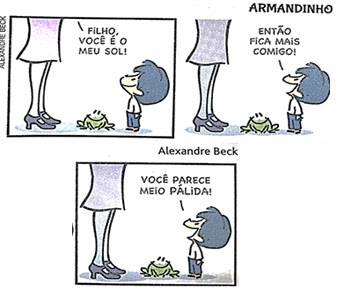
\includegraphics[width=3.51042in,height=3.02083in]{./imgSAEB_7_POR/media/image14.png}

%\fonte{https://tirasarmandinho.tumblr.com/}{\uline{https://tirasarmandinho.tumblr.com/}}.
%Acesso em 20 de Abr de 2023.

\begin{quote}

Desde que a febre de possuir se apoderou de João Romão totalmente, todos os seus atos, todos, 
fosse o mais simples, visavam um interesse pecuniário. Só tinha uma preocupação: aumentar 
os bens. Das suas hortas recolhia para si e para a companheira os piores legumes, aqueles que,
por maus, ninguém compraria; as suas galinhas produziam muito e ele não comia um ovo, do que, 
no entanto, gostava imenso; vendia-os todos e contentava-se com os restos da comida dos 
trabalhadores. Aquilo já não era ambição, era uma moléstia nervosa, uma loucura, um desespero
de acumular; de reduzir tudo a moeda.

\end{quote}

\fonte{Aluísio Azevedo. O cortiço. 
Disponível em: http://objdigital.bn.br/Acervo_Digital/Livros_eletronicos/cortico.pdf}
Acesso em: 22 mai. 2023.}

No trecho acima, o efeito obtido por meio da personificação da ``febre de possuir'' é descrever

\begin{escolha}
  
  \item a simplicidade do trabalhador João Romão. 
  
  \item a miséria de João Romão e sua companheira.
  
  \item a resignação humilde de João Romão. 
  
  \item a ambição João Romão de acumular bens. 

\end{escolha}

\coment{SAEB: Analisar o uso de figuras de linguagem como estratégia argumentativa.

a) Incorreta. O narrador insiste nas ambições de João Romão, não em sua simplicidade.
b) Incorreta. As galinhas de João Romão e sua companheira davam muitos ovos, o que significa 
que ele e a companheira não viviam em miséria.
c) Incorreta. João Romão não se resigna: ele é tomado pela ``a febre de possuir'' para ``aumentar 
os bens''.
d) Correta. O conjunto do trecho insiste em que ``a febre de possuir'' é a personificação da 
ambiçao de João Romão, cujos atos ``visavam um interesse pecuniário'', que só queria ``aumentar 
os bens'' e ``reduzir tudo a moeda''.} 

\chapter{Tecendo com as palavras: recursos de coesão e progressão textual}
\markboth{Módulo 10}{}

\colorsec{Habilidades do SAEB}

\begin{itemize}

  \item Analisar os mecanismos que contribuem para a progressão textual.

  \item Analisar os processos de referenciação lexical e pronominal.

\end{itemize}


\colorsec{Habilidades da BNCC}

\begin{itemize}

  \item EF07LP12, EF07LP13.

\end{itemize}

\conteudo{A coesão textual é um importante recurso da comunicação escrita.
Para que um texto seja bem escrito e bem compreendido, é necessário que
todas as partes e ideias sejam ordenadas de forma organizada, a fim de
produzir um sentido de conjunto. Para integrar ideias e argumentos que 
compõem um texto, alguns recursos são importantes: conjunções e advérbios, 
por exemplo, servem para estabelecer relações entre ideias, parágrafos, 
orações e frases. Em alguns casos, a fluência da leitura pode
exigir o uso de sinônimos, que vão contribuindo com os sentidos do texto e 
com a coesão ao posicionamento do autor. Pronomes também servem para evitar
a repetição de palavras, evitando a monotonia e trazendo maior objetividade ao texto.

Portanto, a coesão textual é essencial para a produção de um texto claro
e de fácil entendimento. Utilizando os recursos adequados, utilizando palavras 
sinônimas e organizando ideias de maneira linear, é possível criar textos coesos
e bem estruturados, capazes de transmitir as informações de forma eficaz de acordo 
com o contexto, o público, a função comunicativa e o gênero textual que se pretende
produzir.}

\coment{Professor(a), converse com os estudantes sobre a coesão textual que
ocorre de maneira imediata na linguagem oral e coloquial. Chame a
atenção para o uso de expressões repetidas tais como ``daí'', ``então'' e ``né'' 
na linguagem coloquial e questione o abuso destes termos e o prejuízo
para a qualidade da comunicação, especialmente a escrita.

Chame a atenção para os diversos tipos, funções e classes gramaticais de
palavras que podem ser usadas a fim de contribuir para estabelecer um
discurso coeso e bem elaborado.}

\colorsec{Atividades}

Leia o texto a seguir para responder às questões de 1 a 3.

\begin{quote}

A Praça da Sé é o centro geográfico da capital paulista. No local está o Marco Zero 
e é partir dele que são medidas as distâncias das rodovias e fronteiras estaduais, 
assim como a numeração das vias públicas da cidade. Junto à praça está situada a 
Catedral Metropolitana da Sé. Em estilo gótico modificado, sua construção iniciou-se em 1913.
É a maior igreja de São Paulo, com capacidade para oito mil pessoas em seus 110m de comprimento, 
46m de largura, além de torres com 92m e cúpula com 30m de altura. Em sua cripta encontram-se
obras do escultor Francisco Leopoldo.

\end{quote}

\fonte{Governo do Estado de São Paulo. Praça da Sé. 
https://www.saopaulo.sp.gov.br/conhecasp/pontos-turisticos/praca-da-se/.
Acesso em: 22 mai. 2023.}

\num{1} Na frase ``No \textbf{local} está o Marco Zero e é partir \textbf{dele} que são medidas
as distâncias das rodovias'', a quem se referem os termos destacados?

\linhas{2}
\coment{Os termos sublinhados se referem, respectivamente, à Praça da Sé e ao Marco Zero.}

\num{2} O nome da cidade a que o autor se refere no trecho ``assim como a numeração das vias 
públicas da \textbf{cidade}'' só aparece depois dessa passagem. Explique que cidade é essa e
como foi possível identificá-la no contexto.

\linhas{6}
\coment{A cidade a que se refere o autor é a cidade de São Paulo, cujo nome só 
aparce depois do trecho destacado. Ele já havia se referido a essa cidade com a expressão ``capital
paulista''. Além disso,  o contexto em que o texto se insere (o site do governo estadual) também
permite inferir que o autor se refere a São Paulo.}

\num{3} Quais foram as expressões usadas pelo autor para referir-se à Catedral da Sé?

\linhas{2}
\coment{Para referir-se à Catedral da Sé, o autor usou o substantivo ``igreja'' e os pronomes 
possessivos em ``sua construção'', ``seus 110m de comprimento'' e ``sua cripta''.}

Leia o texto a seguir para responder às questões 4 e 5.

\begin{quote}

Profissionais da área da educação, da saúde e da assistência social têm
definido ações de cuidado para as comunidades escolares que vivem
situações de violência. Nada fácil, pois a precarização desses setores
tem gerado acúmulo de trabalho e esgotamento.

\end{quote}

\fonte{Adriana Marcondes Machado. Jornal da USP. Violência às escolas: reflexões. 
Disponível em: https://jornal.usp.br/artigos/violencia-as-escolas-reflexoes/.
Acesso em: 22 mai. 2023.}

\num{4} A expressão ``desses setores'' se refere a que outro termos?

\linhas{1}
\coment{A expressão ``desses setores'' se refere às áreas da educação, da saúde e 
da assistência social.}

\num{5} A expressão ``nada fácil'' se refere a que afirmação?

\linhas{2}
\coment{A expressão ``nada fácil'' se refere às ``ações de cuidado para as comunidades escolares que vivem
situações de violência''.}

Leia o texto abaixo para responder às questões de 6 a 8.

\begin{quote}

A professora decidiu dividir os alunos do sétimo ano em dois grupos. De um
lado, aqueles que já haviam realizado a prova; de outro, os estudantes que
haviam faltado e que ainda precisavam realizar o exame. Estes deveriam
ser encaminhados para a sala ao lado. O local estava pronto para receber
os estudantes.

\end{quote}

\num{6} Sublinhe no texto os termos utilizados como recursos de coesão para
evitar repetição dos termos. 

\coment{A professora decidiu dividir os alunos do sétimo ano em dois grupos. De um
lado, \textbf{aqueles} que já haviam realizado a prova; de outro, \textbf{os
jovens} que haviam faltado e que ainda precisavam realizar \textbf{o
exame}. \textbf{Estes} deveriam ser encaminhados para a sala ao lado.
\textbf{O local} estava pronto para receber \textbf{os estudantes.}

\num{7} O termo \textbf{os jovens} se refere a um termo anterior, restringindo-o. 
Explique essa afirmação.

\linhas{5}
\coment{O termo ``os jovens'' se refere ao antecedente ``os alunos'', mas não a todos eles:
apenas aos que haviam faltado.}

\num{8} O pronome \textbf{estes} se refere a qual grupo de estudantes?

\linhas{2}
\coment{O pronome \textbf{estes} se refere aos estudantes que não haviam realizado a prova.}

\num{9}Complete as lacunas com as palavras do quadro.

\begin{table}[]
\begin{tabular}{cc}
obra & garota \\
cujo & ela
\end{tabular}
\end{table}

O livro \_\_\_\_\_\_\_\_ autor Maria conhecia, foi premiado em diversos
concursos literários. A \_\_\_\_\_ tratava das questões que interessavam
a \_\_\_\_\_. A \_\_\_\_\_\_\_\_\_ era uma leitora incansável.

\coment{O livro \textbf{cujo} autor Maria conhecia, foi premiado em diversos
concursos literários. A \textbf{obra} tratava das questões que
interessavam a \textbf{ela}. A \textbf{garota} era uma leitora incansável.}

\num{10} Nas frases abaixo substitua o ponto final por uma conjunção

\begin{escolha}

  \item O clima da cidade é muito árido. Quando vem o período das chuvas a
  vegetação revigora.
  
  \item O engarrafamento no centro da cidade se prolongou. Houve inundações em
  vários pontos.
  
  \item Adoraria viajar nas minhas férias. Não tenho dinheiro para isso.

\end{escolha}

\coment{Apresentamos a seguir algumas possibilidades de redação, mas, como o enunciado
não contém orientação específica, outras redações são possíveis. 

a) O clima da cidade é muito árido, mas, quando vem o período das chuvas, 
a vegetação revigora.

b) O engarrafamento no centro da cidade se prolongou, pois houve
inundações em vários pontos.

c) Adoraria viajar nas minhas férias, mas não tenho dinheiro para isso.}

\colorsec{Treino}

\num{1} Leia o texto abaixo para responder à pergunta.

\begin{quote}

Considerados ``padrão ouro'' nos estudos de saúde, os ensaios clínicos
randomizados controlados, que consistem em testes com voluntários, são a
príncípio aqueles que melhor poderiam mostrar a causalidade entre a
vitamina D e algum efeito na saúde. Mas estudos desse tipo têm
encontrado obstáculos.''

\end{quote}

\fonte{Mariana Alvim. BBC News Brasil. Vitamina D: o que se sabe e o que 
falta saber sobre suplementos, benefícios e riscos. 
Disponível em: https://www.bbc.com/portuguese/articles/c4nzzzz407xo.
Acesso em: 22 mai. 2023.}

A expressão ``aqueles'' se refere ao antecedente:

\begin{escolha}

  \item ``padrão ouro''.
  
  \item ``estudos de saúde''.
  
  \item ``ensaios clínicos randomizados controlados''.
  
  \item ``estudos desse tipo''. 

\end{escolha}

\coment{SAEB: Analisar os processos de referenciação lexical e pronominal.

BNCC: EF07LP12 -- Reconhecer recursos de coesão referencial:
substituições lexicais (de substantivos por sinônimos) ou pronominais
(uso de pronomes anafóricos -- pessoais, possessivos, demonstrativos.

a) Incorreta. O termo se refere à expressão ``ensaios clínicos randomizados controlados''.
b) Incorreta. O termo se refere à expressão ``ensaios clínicos randomizados controlados''.
c) Correta. O termo se refere à expressão ``ensaios clínicos randomizados controlados''. 
d) Incorreta. O termo se refere à expressão ``ensaios clínicos randomizados controlados''.}

\num{2} Leia o texto abaixo para responder à pergunta.

\begin{quote}

A lei alterou as diretrizes e bases da educação nacional para a
inclusão obrigatória do ensino da história e cultura afro-brasileira na
rede pública e particular de ensino fundamental e médio.

\textbf{Conforme o texto}, o conteúdo deve abordar o estudo da história
da África e dos africanos, a luta dos negros no Brasil, a cultura negra
e a participação do negro na formação da sociedade brasileira, nas áreas
social, econômica e política.

\end{quote}

\fonte{R7 Educação. Mais de 70\% das cidades não cumprem o que manda a lei do
ensino afro-brasileiro nas escolas. 
Disponível em: https://noticias.r7.com/educacao/mais-de-70-das-cidades-nao-cumprem-o-que-manda-a-lei-do-ensino-afro-brasileiro-nas-escolas-20042023.
Acesso em: 22 mai. 2023.}

O trecho em destaque se refere ao antecedente:

\begin{escolha}
  
  \item ``a lei''.
  
  \item ``ensino da história e cultura afro-brasileira''.
  
  \item ``estudo da história da África e dos africanos''.
  
  \item ``a participação do negro na formação da sociedade brasileira''.

\end{escolha}

\coment{SAEB:Analisar os mecanismos que contribuem para a progressão textual.

BNCC: EF07LP12 -- Reconhecer recursos de coesão referencial:
substituições lexicais (de substantivos por sinônimos) ou pronominais
(uso de pronomes anafóricos -- pessoais, possessivos, demonstrativos.

a) Correta. O termo ``o texto'' se refere a ``a lei''.
b) Incorreta. O termo ``o texto'' se refere a ``a lei''.  
c) Incorreta. O termo ``o texto'' se refere a ``a lei''. 
d) Incorreta. O termo ``o texto'' se refere a ``a lei''.}

\num{3} Leia o texto abaixo para responder à pergunta.

\begin{quote}

Era uma vez um lobo vegano que não engolia a vovozinha, três
porquinhos que se dedicavam à especulação imobiliária e uma estilista
chamada Gretel que trabalhava de garçonete em Berlim. Não deveria nos
surpreender que os contos tradicionais se adaptem aos tempos. Eles foram
submetidos a alterações no processo de transmissão, oral ou escrita, ao
longo dos séculos para adaptá-los aos gostos de cada momento.

\end{quote}

\fonte{Marta Rebós. El País Brasil. O lobo devorou, sim, a Chapeuzinho. 
https://brasil.elpais.com/brasil/2018/09/18/eps/1537265048_460929.html
Acesso em: 22 mai. 2023.}

No útlimo período do texto, os termos destacados em ``\textbf{Eles} foram
submetidos a alterações'' e ``para adaptá-\textbf{los} aos gostos'' se referem:

\begin{escolha}

  \item aos antecedentes ``lobo vegano'' e ``três porquinhos''.

  \item ambos ao antecedente ``três porquinhos''. 

  \item ambos ao antecedente ``contos tradicionais''.

  \item aos antecedentes ``contos tradicionais'' e ``séculos''.

\end{escolha}

\coment{SAEB: Analisar os processos de referenciação lexical e pronominal.

BNCC: EF07LP12 -- Reconhecer recursos de coesão referencial:
substituições lexicais (de substantivos por sinônimos) ou pronominais
(uso de pronomes anafóricos -- pessoais, possessivos, demonstrativos.

a) Incorreta. ``Eles'' e ``-los'' se referem ao antecedente ``contos tradicionais''.
b) Incorreta. ``Eles'' e ``-los'' se referem ao antecedente ``contos tradicionais''.
c) Correta. ``Eles'' e ``-los'' se referem ao antecedente ``contos tradicionais''.
d) Incorreta. ``Eles'' e ``-los'' se referem ao antecedente ``contos tradicionais''.}

\chapter{Variedades linguísticas}
\markboth{Módulo 11}{}

\colorsec{Habilidades do SAEB}

\begin{itemize}

  \item Analisar as variedades linguísticas em textos.

  \item Avaliar a adequação das variedades linguísticas em contextos de uso.

\end{itemize}

\colorsec{Habilidades da BNCC}

\begin{itemize}

  \item EF69LP55, EF69LP56.

\begin{itemize}

\conteudo{A língua é um fenômeno social complexo que se manifesta de diversas
maneiras, de acordo com o contexto. As várias
formas de uso da língua são chamadas de \textbf{variedades linguísticas}, e estão
presentes nas diferenças de pronúncia, vocabulário e situação
comunicativa.

Existem muitas variações da língua falada, pois a linguagem é
influenciada por fatores como a região onde se encontram determinadas
expressões, o nível de escolaridade, a idade, a classe social e a etnia
dos falantes. As variações linguísticas podem ser referentes
ao uso coloquial ou formal, ao uso profissional, ou depender de aspectos
geográficos e históricos. Por esses motivos, as variações
se diferenciam da chamada norma-padrão.

Contudo, mesmo que a diversidade seja uma característica
inerente à linguagem, as variações linguísticas podem sofrer preconceitos
e discriminação. Por outro lado, conhecê-las permite a criação de um
discurso mais acessível e atento ao público a que se dirige. No entanto,
considerar determinadas formas de uso da língua inferiores ou
equivocadas pode ser considerado preconceito linguístico.

O preconceito linguístico pode ter diversas consequências negativas,
como a exclusão social de falantes de determinadas variedades
linguísticas, pois não são levados em conta diversos fatores como a
dificuldade de acesso e de oportunidades educacionais e profissionais.

Portanto, é importante valorizar e respeitar a diversidade linguística
como um patrimônio cultural e expressivo que considera todos os falantes
da língua, combatendo os preconceitos e promovendo a inclusão social.}

\colorsec{Atividades}


\num{1} Quais são os fatores que devem ser considerados para compreender as
variações linguísticas existentes entre os falantes de uma mesma

\reduline{Para compreender as variações linguísticas, é preciso levar em 
consideração fatores sociais, nível de escolaridade, poder aquisitivo, 
peculiaridades culturais, étnicas e regionais.} 

\num{2} Por que a desvalorização de determinados usos da linguagem pode ser
considerada preconceito?

\reduline{A desconsideração das questões que promovem as variações linguísticas
induz ao preconceito, pois não se pode desconsiderar o contexto do
emissor e nem a situação comunicativa. Em muitos casos, a norma-padrão
não se apresenta como a forma mais eficaz de elaborar um texto ou
discurso. Além disso, a norma-padrão pode servir à manutenção da desigualdade
social, especialmente em países como o Brasil.} 

Leia um trecho do romance \textit{Dom Casmurro}, de Machado de Assis:

Capitu deixou-se ir, rindo; depois a conversa entrou a cochilar e
dormir. Tínhamos chegado à janela; um preto, que, desde algum
tempo, vinha apregoando cocadas, parou em frente e perguntou:

--- Sinhazinha, qué cocada hoje?

--- Não, respondeu Capitu.

--- Cocadinha tá boa.

--- Vá-se embora, replicou ela sem rispidez.

--- Dê cá! disse eu descendo o braço para receber duas.

Comprei-as, mas tive de as comer sozinho; Capitu recusou. Vi
que, em meio da crise, eu conservava um canto para as cocadas, o
que tanto pode ser perfeição como imperfeição, mas o momento
não é para definições tais; fiquemos em que a minha amiga,
apesar de equilibrada e lúcida, não quis saber de doce, e gostava
muito de doce. Ao contrário, o pregão que o preto foi cantando, o
pregão das velhas tardes, tão sabido do bairro e da nossa infância:

\begin{verse}
Chora, menina, chora, \\
Chora, porque não tem \\
Vintém
\end{verse}
\end{quote}

\fonte{Machado de Assis. Dom Casmurro. 
Disponível em: https://www.ic.unicamp.br/~stolfi/misc/2012-02-13-domine-casmurrus.pdf.
Acesso em: 22 mai. 2023.}

\num{3} No diálogo entre o vendedor de cocadas, de um lado, e Capitu e Bentinho, 
o narrador do romance, de outro, é possível perceber variações linguísticas. 
Explique essas variações, considerando que, no período em que se passa o romance, o 
vendedor é uma pessoa escravizada no Brasil de meados do século XIX, ao contrário do 
narrador e Capitu, que são brancos com acesso à educação formal. 

\reduline{Fica evidente no diálogo entre o vendedor de cocadas e Capitu e Bentinho que
o abismo social entre essas personagens se manifesta nas variações linguísticas. Enquanto
as falas de Capitu e Bentinho tendem à norma-padrão (por exemplo, no uso do pronome em 
``vá-se embora''), as do vendedor se aproximam da informalidade oral, como em 
``qué cocada hoje?'' e ``Cocadinha tá boa''.}

\num{4} Nos parágrafos do narrador, qual é a variedade linguística predominante? 
Copie um exemplo de uso de pronomes que confirma essa explicação. 

\reduline{O uso dos pronomes pessoais oblíquos átonos em ``Comprei-as, mas tive de 
as comer sozinho'' corresponde à norma-padrão. Em variedade linguística menos rigorosa,
e mais natural para muitos falantes de língua portuguesa do Brasil, seria usado o pronome
``elas''.} 

\num{5} O que são os \textbf{pregões} citados pelo narrador? Ainda existem pregões no
seu cotidiano? Se sim, explique; se não, levante hipóteses sobre o desaparecimento dessa 
prática.

\reduline{Pregões são divulgações em voz alta de produtos à venda, por vendedores ambulantes. 
Feirantes de rua ainda costumam usar pregões, bem como vendedores ambulantes nas praias de 
todo o Brasil. Contudo, o ambiente do comércio em shopping centers, mais formal, não contempla
essa prática.} 

%Analise a tirinha e responda:

%
\includegraphics[width=5.90551in,height=1.70833in]{./imgSAEB_7_POR/media/image15.png}

%\num{6}
%  A tirinha apresenta um tipo de variação linguística? Justifique sua resposta
%\end{enumerate}

%Sim. A tirinha apresenta uma variação linguística pois apresenta vários
%nomes de um mesmo vegetal, cada forma é utilizada em uma região
%diferente do país

%\num{7}
%  Alguma das formas mandioca, aipim ou macaxeira pode ser considerada
%  mais correta do que as outras? Por que?
%\end{enumerate}

%Não, pois cada região possui suas formas de falar, suas gírias e
%expressões e muitas vezes, podem haver vários sinônimos em uma mesma
%língua usado em regiões e culturas diferentes.

\num{6} Na tabela a seguir, assinale (V) para as afirmações verdadeiras e (F) para as falsas no que
se refere às variedades linguísticas. 

% Please add the following required packages to your document preamble:
% \usepackage[table,xcdraw]{xcolor}
% If you use beamer only pass "xcolor=table" option, i.e. \documentclass[xcolor=table]{beamer}
\begin{table}[]
\begin{tabular}{|c|c|}
\hline
\rowcolor[HTML]{DAE8FC} 
\textbf{\begin{tabular}[c]{@{}c@{}}Verdadeiro (V)\\ ou \\ Falso (F)\end{tabular}} & \textbf{Afirmação} \\ \hline
 & toda situação comunicativa exige o uso da norma-padrão \\ \hline
\rowcolor[HTML]{ECF4FF} 
 & \begin{tabular}[c]{@{}c@{}}o uso da norma-padrão é mais adequado para a redação de\\ documentos oficiais, textos de lei e petições\end{tabular} \\ \hline
 & textos literários devem sempre fazer uso da norma-padrão \\ \hline
\rowcolor[HTML]{ECF4FF} 
 & \begin{tabular}[c]{@{}c@{}}em algumas situações, é mais adequado não \\ utilizar a norma-padrão\end{tabular} \\ \hline
 & \begin{tabular}[c]{@{}c@{}}a escolha pelo uso da norma-padrão ou de variações que se distanciam dela\\ deve orientar-se pelo contexto da comunicação\end{tabular} \\ \hline
\end{tabular}
\end{table}

\coment{F, V, F, V, V}

\num{7} Na tabela abaixo, assinale com um X os gêneros textuais em que o uso da norma-padrão 
tende a ser mais adequado.

% Please add the following required packages to your document preamble:
% \usepackage[table,xcdraw]{xcolor}
% If you use beamer only pass "xcolor=table" option, i.e. \documentclass[xcolor=table]{beamer}
\begin{table}[]
\begin{tabular}{c|c|}
\cline{2-2}
\rowcolor[HTML]{FFFFFF} 
\textbf{} & \cellcolor[HTML]{DAE8FC}\textbf{gêneros textuais} \\ \hline
\multicolumn{1}{|c|}{} & cartas pessoais \\ \hline
\rowcolor[HTML]{ECF4FF} 
\multicolumn{1}{|c|}{\cellcolor[HTML]{ECF4FF}} & cartas abertas à sociedade \\ \hline
\multicolumn{1}{|c|}{} & petições \\ \hline
\rowcolor[HTML]{ECF4FF} 
\multicolumn{1}{|c|}{\cellcolor[HTML]{ECF4FF}} & textos de divulgação científica \\ \hline
\multicolumn{1}{|c|}{} & leis e estatutos \\ \hline
\multicolumn{1}{|c|}{} & poemas \\ \hline
\end{tabular}
\end{table}

\coment{% Please add the following required packages to your document preamble:
% \usepackage[table,xcdraw]{xcolor}
% If you use beamer only pass "xcolor=table" option, i.e. \documentclass[xcolor=table]{beamer}
\begin{table}[]
\begin{tabular}{c|c|}
\cline{2-2}
\rowcolor[HTML]{FFFFFF} 
\textbf{} & \cellcolor[HTML]{DAE8FC}\textbf{gêneros textuais} \\ \hline
\multicolumn{1}{|c|}{} & cartas pessoais \\ \hline
\rowcolor[HTML]{ECF4FF} 
\multicolumn{1}{|c|}{\cellcolor[HTML]{ECF4FF}\textbf{X}} & cartas abertas à sociedade \\ \hline
\multicolumn{1}{|c|}{X} & petições \\ \hline
\rowcolor[HTML]{ECF4FF} 
\multicolumn{1}{|c|}{\cellcolor[HTML]{ECF4FF}X} & textos de divulgação científica \\ \hline
\multicolumn{1}{|c|}{X} & leis e estatutos \\ \hline
\multicolumn{1}{|c|}{} & poemas \\ \hline
\end{tabular}
\end{table}
}

\num{8} Na tabela abaixo, assinale com um X as situações comunicativas em que tende a ser mais adequado
o uso da linguagem coloquial.

% Please add the following required packages to your document preamble:
% \usepackage[table,xcdraw]{xcolor}
% If you use beamer only pass "xcolor=table" option, i.e. \documentclass[xcolor=table]{beamer}
\begin{table}[]
\begin{tabular}{c|c|}
\cline{2-2}
\rowcolor[HTML]{FFFFFF} 
\textbf{} & \cellcolor[HTML]{DAE8FC}\textbf{situações comunicativas} \\ \hline
\multicolumn{1}{|c|}{} & conversa com amigos \\ \hline
\rowcolor[HTML]{ECF4FF} 
\multicolumn{1}{|c|}{\cellcolor[HTML]{ECF4FF}\textbf{}} & matérias de jornal \\ \hline
\multicolumn{1}{|c|}{} & \begin{tabular}[c]{@{}c@{}}apresentação de \\ trabalho escolar\end{tabular} \\ \hline
\rowcolor[HTML]{ECF4FF} 
\multicolumn{1}{|c|}{\cellcolor[HTML]{ECF4FF}} & mensagens em redes sociais \\ \hline
\end{tabular}
\end{table}

\coment{% Please add the following required packages to your document preamble:
% \usepackage[table,xcdraw]{xcolor}
% If you use beamer only pass "xcolor=table" option, i.e. \documentclass[xcolor=table]{beamer}
\begin{table}[]
\begin{tabular}{c|c|}
\cline{2-2}
\rowcolor[HTML]{FFFFFF} 
\textbf{} & \cellcolor[HTML]{DAE8FC}\textbf{situações comunicativas} \\ \hline
\multicolumn{1}{|c|}{X} & conversa com amigos \\ \hline
\rowcolor[HTML]{ECF4FF} 
\multicolumn{1}{|c|}{\cellcolor[HTML]{ECF4FF}\textbf{}} & matérias de jornal \\ \hline
\multicolumn{1}{|c|}{} & \begin{tabular}[c]{@{}c@{}}apresentação de \\ trabalho escolar\end{tabular} \\ \hline
\rowcolor[HTML]{ECF4FF} 
\multicolumn{1}{|c|}{\cellcolor[HTML]{ECF4FF}X} & mensagens em redes sociais \\ \hline
\end{tabular}
\end{table}
}

\colorsec{Treino}

\num{1} Leia os versos do coco abaixo para responder à questão.

\begin{quote}
\begin{verse}

Eu vi uma lagartixa \\
Ai, tava numa jinela, \\
Ai, dizeno que era honrada, \\
Que era moça donzela, \\
Vi quat' calango verde, \\
Tudo era fio dela. 

\end{verse}
\end{quote}

\fonte{Mário de Andrade. Os cocos. Belo Horizonte: Itatiaia, 2002. p. 157.} 

O coco é uma dança popular de roda, que se executa ao som de canto, batida de palmas e 
toque de percussão. Nos versos acima, registrados pelo escritor e pesquisador Mário de 
Andrade, observa-se a transcrição da fala coloquial em:

\begin{escolha}
  
  \item ``eu vi''.
  
  \item ``era honrada''.
  
  \item ``donzela''.
  
  \item ``fio dela''

\end{escolha}

\coment{SAEB: Avaliar a adequação das variedades linguísticas em contextos de uso.

a) Incorreta. A transcrição da fala popular se observa em ``fio dela'', equivalente a ``filho dela''.
b) Incorreta. A transcrição da fala popular se observa em ``fio dela'', equivalente a ``filho dela''.
c) Incorreta. A transcrição da fala popular se observa em ``fio dela'', equivalente a ``filho dela''.
d) Correta. A transcrição da fala popular se observa em ``fio dela'', equivalente a ``filho dela''.} 

\num{2} Leia o texto abaixo para responder à questão.

\begin{quote}
Nota-se também que as diferentes regiões brasileiras não apresentam um
cenário socioeconômico igual, o que afeta a frequência do câncer e de
outras doenças. ``Pensar em regionalização é essencial. Nas regiões Norte
e Nordeste, por exemplo, esse tipo de câncer não é tão frequente como em
outros espaços do País. Quando você pensa em um projeto de prevenção, é
necessário pensar em regionalização'', discorre Hoff.''
\end{quote}

\fonte{Jornal da USP. Câncer de intestino já é mais comum em grupos de pessoas mais jovens.
Disponível em: https://jornal.usp.br/radio-usp/cancer-de-intestino-ja-e-mais-comum-em-grupos-de-pessoas-mais-jovens/.
Acesso em: 22 mai. 2023.}

No exemplo acima, o autor usou da norma-padrão para adequar-se à linguagem apropriada ao texto

\begin{escolha}
  
  \item literário.
  
  \item humorístico.
  
  \item jornalístico.
  
  \item jurídico.

\end{escolha}

\coment{Saeb:Avaliar a adequação das variedades linguísticas em contextos de
uso.

a) Incorreta. O texto da questão é jornalístico. 

b) Incorreta. O texto da questão é jornalístico. 

c) Correta. O texto da questão é jornalístico, por isso o autor optou pelo uso da norma-padrão. 

d) Incorreta. O texto da questão é jornalístico.}

\num{3} Leia o trecho do romance \textit{A Família Medeiros}, de Júlia Lopes de Almeida para 
respoder à questão. 

\begin{quote}

Passada a curva do jequitibá grande, topou com um negro
que vencia o morro a largas passadas e que o saudou com um
soturno:
--- Sum Cristo!
--- Sabe-me dizer se há algum atalho novo para a Fazenda de
Santa Genoveva?
--- Prá o sito do coroné Medêro? Não há não, sinhô. Eu
também tô indo prá lá.
E atentando em Otávio:
--- A modo qui tô conhecendo mecê \ldots{}
--- Está, sim. E você, como se chama?
--- Me chamo Antonho; fio de Luzia pernambucana, sim sinhô.
--- Foi a algum recado à cidade?
--- Fui na vila buscá rémedio pró fio do feitô, qui foi moldido
de cobra, sim sinhô \ldots{}
--- Ah, então apresse-se --- disse Otávio, para dizer alguma
coisa, e tocou o animal para diante.

\fonte{Júlia Lopes de Almeida. A Família Medeiros. São Paulo: Editora Hedra. no prelo.}

No diálogo acima, observa-se a transcrição da fala coloquial em:

\begin{escolha}
  
  \item ``vencia o morro a largas passadas''.
  
  \item ``Sabe-me dizer se há algum atalho novo''. 
  
  \item ``A modo qui tô conhecendo mecê''.
  
  \item ``então apresse-se''. 

\end{escolha}

\coment{SAEB: Analisar as variedades linguísticas em textos.

a) Incorreta. A transcrição da fala popular se observa em ``A modo qui tô conhecendo mecê''.
b) Incorreta. A transcrição da fala popular se observa em ``A modo qui tô conhecendo mecê''. 
c) Incorreta. A transcrição da fala popular se observa em ``A modo qui tô conhecendo mecê''. 
d) Incorreta. A transcrição da fala popular se observa em ``A modo qui tô conhecendo mecê''.} 

\chapter{Simulado 1}
\markboth{Simulado 1}{}

\num{1} Observe o cartaz abaixo para responder à questão.

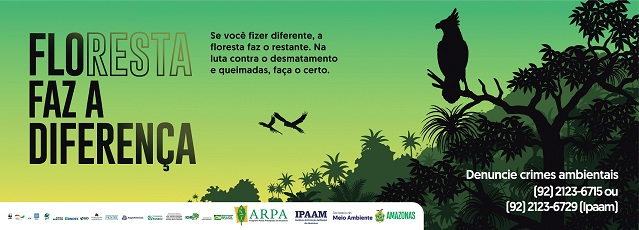
\includegraphics[width=5.90551in,height=2.125in]{./imgSAEB_7_POR/media/image16.png}

\fonte{Secretaria do Meio Ambiente do Estado do Amazonas. Campanha Floresta faz a diferença. 
Disponível em: https://meioambiente.am.gov.br/campanha-floresta-faz-a-diferenca/.
Acesso em: 22 mai. 23}

Acima, pode-se observar um cartaz de conscientização sobre o desmatamento da
Amazônia. O uso e repetição de determinadas palavras e imagens tem como
finalidade sensibilizar os leitores para o problema do desmatamento.
Sobre o uso da palavra ``floresta'', no cartaz, assinale a alternativa
correta.

\begin{escolha}

  \item Destacada à esquerda em letras grandes, uma parte da palavra ``floresta'' compõe um jogo com 
  palavras do texto no centro do cartaz.   

  \item A parte destacada da palavra ``floresta'', à esquerda, remete aos malefícios das queimadas e desmatamento
  que o cartaz pretende combater. 

  \item O destaque da palavra ``floresta'' não dialoga com ``diferença'' e ``diferente'', que se articulam para convidar a uma mudança de atitude.

  \item O uso da palavra ``floresta'', em destaque, à esquerda, dialoga com as imagens à direita sem remeter ao texto central do cartaz da campanha. 

\end{escolha}

\coment{SAEB: Identificar o uso de recursos persuasivos em textos verbais e
não verbais.

BNCC: EF67LP07 -- Identificar o uso de recursos persuasivos em textos
argumentativos diversos (como a elaboração do título, escolhas lexicais,
construções metafóricas, a explicitação ou a ocultação de fontes de
informação) e perceber seus efeitos de sentido.

a) Correta. A parte de palavra ``resta'' dialoga com a frase ``se você fizer diferente, a floresta faz o
restante'': \textit{resta} e \textit{restante} dizem respeito ao papel da \textit{floresta}.     
b)Incorreta. A parte destacada da palavra ``floresta'' não remete aos malefícios das queimadas e desmatamento, 
mas ao contrário: \textit{resta} e \textit{restante} dizem respeito ao papel da \textit{floresta}. 
c)Incorreta. O destaque da palavra ``floresta'' dialoga com ``diferença'' e ``diferente'': se as pessoas fizerem
diferente, a floresta faz o \textit{restante}, palavra que remete à parte da palavra ``floresta'', destacada 
à esquerda. 
d)Incorreta. O uso da palavra ``floresta'' certamente dialoga com as imagens à direita e com o texto central do cartaz da campanha.}

\num{2} Leia o texto abaixo para responder à questão. 

\begin{quote}
\textbf{Fumaça de queimadas do Amazonas chega a São Paulo; moradores
relatam ``cheiro forte''}

\textit{Segundo a Climatempo, a nuvem de fumaça foi gerada por incêndios em
parte do Amazonas, Acre e Mato Grosso.}

Moradores da cidade de São Paulo relataram sentir cheiro de fumaça na
manhã desta sexta-feira (9).

Na quinta (8), a Climatempo havia alertado para a nuvem gerada por
queimadas em parte do Amazonas, Acre e Mato Grosso, que se espalhou sobre o
Brasil, e que chegaria também em grande parte do Centro-Oeste, no Paraná
e até em parte do estado de São Paulo.

A Companhia Ambiental do Estado de São Paulo (CETESB) disse que a
Divisão de Qualidade do Ar da agência está investigando as fumaças e
monitorando a qualidade do ar.

``A divisão está fazendo uma apuração detalhada dos dados das
estações de monitoramento da qualidade do ar distribuídas pela RMSP
Informaremos assim que tivermos um dado mais consolidado sobre a
ocorrência'', diz a nota.
\end{quote}

\fonte{Ingrid Oliveira e Carolina Figueiredo. Fumaça de queimadas do Amazonas chega a São Paulo; 
moradores relatam “cheiro forte”. Disponível em:
https://www.cnnbrasil.com.br/nacional/fumaca-de-queimadas-do-amazonas-chega-a-sao-paulo-moradores-relatam-cheiro-forte/.
Acesso em: 22 mai. 2023.}

Assinale a alternativa que contém a parte da notícia denominada linha fina.

\begin{escolha}

\item Fumaça de queimadas do Amazonas chega a São Paulo; moradores relatam ``cheiro forte''.

\item A divisão está fazendo uma apuração detalhada dos dados das estações de monitoramento.

\item Moradores da cidade de São Paulo relataram sentir cheiro de fumaça na manhã desta sexta-feira (9).

\item Segundo a Climatempo, a nuvem de fumaça foi gerada por incêndios em parte do Amazonas, Acre e Mato Grosso.

\end{escolha}

\coment{SAEB: Identificar elementos constitutivos de textos pertencentes ao
domínio jornalístico/midiático.

a) Incorreta. O trecho corresponde ao título da notícia.
b) Incorreta. O trecho pertence ao corpo da notícia.
c) Incorreta. O trecho pertence ao corpo da notícia.
d) Correta. A linha fina aparece como uma introdução ao assunto da notícia, logo depois do título.}

\num{3} Leia o texto abaixo para responder à questão.

\begin{quote}
Uma parceria entre a Universidade Federal do Rio de Janeiro e a
Universidade Federal do Estado do Rio de Janeiro (Unirio) vem estudando
o vírus-T linfotrópico humano do tipo 1, o HTLV-1, retrovírus da mesma
família do HIV, associado a casos de leucemia e doenças
neurodegenerativas. A pesquisa recebeu investimento da Organização
Pan-Americana de Saúde (Opas/OMS) junto com outros estudos
latino-americanos e caribenhos que investigam doenças negligenciadas.
Embora descrito, na década de 1980, como um vírus associado ao câncer, o
HTLV ainda é pouco estudado e bastante desconhecido do público em geral.
\end{quote}

\fonte{Carol Correia e Luana Reis.Conexão UFRJ. 
Pesquisa investiga vírus que pode levar à leucemia e neurodegeneração.
Disponível em: https://conexao.ufrj.br/2023/04/pesquisa-investiga-virus-negligenciado-que-pode-levar-a-doencas-neurodegenerativas-e-leucemia/.
Acesso em: 22 mai. 2023.}

O texto acima pertence ao gênero de divulgação científica, pois:

\begin{escolha}
  
  \item traz informações técnicas e de difícil compreensão.
  
  \item é escrito de maneira formal e dirigido a cientistas e estudiosos.
  
  \item traz informações sobre fatos do cotidiano.
  
  \item traz informações científicas em linguagem clara e acessível ao público
  geral.

\end{escolha}

\coment{SAEB: Identificar elementos constitutivos de gêneros de divulgação científica

a) Incorreta. O texto não apresenta linguagem técnica. 
b) Incorreta. O texto não é destinado apenas a cientistas.
c) Incorreta. O trecho não aborda fatos cotidianos. 
d) Correta. O texto faz uso de linguagem clara e acessível para divulgar estudos científicos
para o público em geral.}

\num{4} Leia o texto abaixo para responder à questão.

\begin{quote}

Ilma. Sra. Diretora da Escola Estadual Ulysses Guimarães:

Mariana Amaral Santos, aluna regularmente matriculada no sétimo ano do
Ensino Fundamental desta escola, vem respeitosamente solicitar à V.S.\textsuperscript{a} a
expedição dos documentos necessários à sua transferência para outro
estabelecimento de ensino.

Nestes termos, pede deferimento.

Curitiba, 24 de setembro de 2022.

\end{quote}

\fonte{Texto adaptado para este material.}

Os gêneros textuais reivindicatórios são textos que circulam no campo da
vida pública e possuem função social e estrutura específicas. O texto
acima é um modelo de Requerimento pois tem como objetivo:

\begin{escolha} 

\item convencer o destinatário a realizar uma ação importante.

\item solicitar formalmente ao destinatário a realização de uma ação.

\item mudar o comportamento do destinatário a partir da realização de ações.

\item informar formalmente o destinatário acerca da solicitação de ações.

\end{escolha}

\coment{SAEB: Identificar formas de organização de textos normativos, legais e/ou
reivindicatórios.

BNCC: EF67LP17 -- Analisar, a partir do contexto de produção, a forma de
organização das cartas de solicitação e de reclamação (datação, forma de
início, apresentação contextualizada do pedido ou da reclamação, em
geral, acompanhada de explicações, argumentos e/ou relatos do problema,
fórmula de finalização mais ou menos cordata, dependendo do tipo de
carta e subscrição) e algumas das marcas linguísticas relacionadas à
argumentação, explicação ou relato de fatos, como forma de possibilitar
a escrita fundamentada de cartas como essas ou de postagens em canais
próprios de reclamações e solicitações em situações que envolvam
questões relativas à escola, à comunidade ou a algum dos seus membros.


a) Incorreta. O texto não tem a pretensão de convencer o leitor.
b) Correta. O texto contém solicitação de transferência de instituição.
c) Incorreta. Não há referência sobre expctativa de mudança de atitude do leitor. 
d) Incorreta. O objetivo da carta não é informar, mas solicitar transferência de instituição.}

\num{5} Leia o texto abaixo para responder à questão.

\begin{quote}
\textbf{ATO I}

\textbf{Cena I}

\textit{Veneza. Uma rua. Entram Antônio, Salarino e Salânio.}

ANTÔNIO -- Não sei, realmente, porque estou tão triste. Isso me enfara; e
a vós também, dissestes. Mas como começou essa tristeza, de que modo a
adquiri, como me veio, onde nasceu, de que matéria é feita, ainda estou
por saber. E de tal modo obtuso ela me deixa, que mui dificilmente me
conheço.

SALARINO -- Vosso espírito voga em pleno oceano, onde vossos galeões de
altivas velas -- como burgueses ricos e senhores das ondas, ou qual vista
aparatosa distendida no mar -- olham por cima da multidão de humildes
traficantes que os saúdam, modestos, inclinando-se, quando perpassam com
tecidas asas.

\end{quote}

\fonte{William Shakespeare. O Mercador de Venza. 
Disponível em: http://www.dominiopublico.gov.br/download/texto/cv000094.pdf.
Acesso em: 22 mai. 2023.}

O trecho acima apresenta certas características, como discurso direto,
indicações de falas de personagens e rubricas, que são características 

\begin{escolha}

  \item das peças de teatro, textos escritos para encenação.

  \item dos poemas, compostos por versos e estrofes.

  \item dos contos, narrações curtas e de alto impacto.

  \item dos romances, narrativa longas e complexas.

\end{escolha}

\coment{SAEB: Analisar elementos constitutivos de textos pertencentes ao domínio literário.

a) Correta. O texto do exercício é parte de uma peça de teatro, com discurso direto, indicação
de personagens e rubricas.
b) Incorreta. O texto do exercício é parte de uma peça de teatro, com discurso direto, indicação
de personagens e rubricas.
c) Incorreta. O texto do exercício é parte de uma peça de teatro, com discurso direto, indicação
de personagens e rubricas.
d) Incorreta. O texto do exercício é parte de uma peça de teatro, com discurso direto, indicação
de personagens e rubricas.}

\num{6} Leia o texto abaixo para responder à questão. 

\begin{quote}

Rogério Ceni deixou o São Paulo. Este é só mais um capítulo na história
de um clube que caminha a passos largos rumo ao buraco. A verdade é uma
só e dói para o apaixonado torcedor admitir: aquele São Paulo que era
modelo de administração e que num intervalo de três anos ganhou
Paulista, Libertadores, Mundial de Clubes e o tricampeonato brasileiro
acabou. Virou apenas lembrança.

\end{quote}

\fonte{Marcelo Prado. G1. Opinião: vaidade e soberba de dirigentes afundam o São Paulo rumo a um futuro preocupante. Disponível em: https://ge.globo.com/futebol/times/sao-paulo/noticia/2023/04/20/opiniao-vaidade-e-soberba-de-dirigentes-afundam-o-sao-paulo-rumo-a-um-futuro-preocupante.ghtml.
Acesso em: 23 mai. 2023.}

O texto acima contém muitas opiniões e poucos fatos. Há um fato
expresso no texto em:

\begin{escolha}

  \item ``Este é só mais um capítulo na história de um clube''.
  
  \item ``A verdade é uma só e dói para o apaixonado torcedor''.
  
  \item ``um clube que caminha a passos largos rumo ao buraco''.
  
  \item ``O São Paulo num intervalo de três anos ganhou Paulista''.

\end{escolha}

\coment{Saeb: Distinguir fatos de opiniões em textos.
 
a) Incorreta. Este trecho representa a opinião do jornalista.
b) Incorreta. Este trecho representa a opinião do jornalista.
c) Incorreta. Este trecho representa a opinião do jornalista.
d) Correta. Este trecho apresenta um fato.}

\num{7} Leia o texto abaixo para responder à questão.

%Alterei a questão. Rogério, 24/5/23, 10h13
%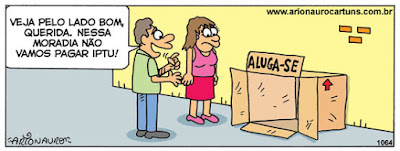
\includegraphics[width=4.16667in,height=1.57292in]{./imgSAEB_7_POR/media/image17.png}
%\fonte{http://www.arionaurocartuns.com.br/search?q=moradia}{\uline{http://www.arionaurocartuns.com.br/search?q=moradia}}.
%Acesso em 20 de Abr de 2023.

\begin{quote}

É inútil descrever o quarto de um estudante: aí nada se
encontra de novo. Ao muito acharão uma estante, onde ele guarda
os seus livros, um cabide, onde pendura a casaca, o moringue, o
castiçal, a cama, uma até duas canastras de roupa, o chapéu, a
bengala e a bacia, a mesa, onde escreve e que só apresenta de
recomendável a gaveta cheia de papéis, de cartas de família, de
flores e fitinhas misteriosas: é pouco mais ou menos assim o
quarto de Augusto.

Agora ele está só. Às sete horas, desse quarto saíram três
amigos: Filipe, Leopoldo e Fabrício. Trataram da viagem no dia 
seguinte e retiraram-se descontentes.

\end{quote}

\fonte{Joaquim Manuel de Macedo. A moreninha. 
Disponível em: http://objdigital.bn.br/Acervo_Digital/Livros_eletronicos/a_moreninha.pdf.
Acesso em: 24 mai. 2023.}

Assinale a alternativa correta quanto aos trechos do texto.

\begin{escolha}
    
    \item ``\textbf{aí} nada se encontra de novo'': o termo destacado se refere a ``um estudante''.
    
    \item ``onde escreve'': o sentido da frase equivale a ``onde eles escrevem''.  
    
    \item ``o quarto de Augusto'': Augusto é o estudante cujo quarto é citado no início do parágrafo.  
    
    \item ``Agora \textbf{ele} está só'': o termo destacado refere-se a ``o quarto de Augusto''.   

\end{escolha}

\coment{SAEB: Inferir, em textos multissemióticos, efeitos de humor, ironia e/ou
crítica.

BNCC: EF69LP03 -- Inferir e justificar, em textos multissemióticos --
tirinhas, charges, memes, gifs etc. --, o efeito de humor, ironia e/ou
crítica pelo uso ambíguo de palavras, expressões ou imagens ambíguas, de
clichês, de recursos iconográficos, de pontuação etc.

a) Incorreta. No trecho ``\textbf{aí} nada se encontra de novo'', o termo destacado se refere a 
``o quarto de um estudante''.
b) Incorreta. No trecho ``onde escreve'': o sentido da frase não equivale a ``onde eles escrevem''.
Pela coesão e coerência do texto, nota-se que a frase equivale a ``onde ele (o estudante) escreve''.
c) Correta. Pela coesão e coerência do texto, verifica-se que, no trecho ``o quarto de Augusto'', 
Augusto é o estudante cujo quarto é citado no início do parágrafo.  
d) Incorreta. No trecho ``Agora \textbf{ele} está só'': o termo destacado refere-se a Augusto.}   

\num{8} Leia o texto abaixo para responder à questão. 

%Tirei a imangem abaixo e alterei a questão (Rogério, 24/5/23, 9h52)
%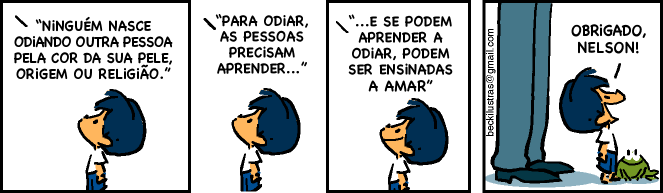
\includegraphics[width=5.90551in,height=1.72222in]{./imgSAEB_7_POR/media/image18.png}
%\fonte{https://tirasarmandinho.tumblr.com/search/amor}{\uline{https://tirasarmandinho.tumblr.com/search/amor}}.
%Acesso em 21 de Abr.

\begin{quote}

--- Não diga isso, Camilo. Se você soubesse como eu tenho andado, por sua
causa. Você sabe; já lhe disse. Não ria de mim, não ria \ldots{}

Camilo pegou-lhe nas mãos, e olhou para ela sério e fixo. Jurou que lhe
queria muito, que os seus sustos pareciam de criança; em todo o caso,
quando tivesse algum receio, a melhor cartomante era ele mesmo. Depois,
repreendeu-a; disse-lhe que era imprudente andar por essas casas.

\end{quote}

\fonte{Machado de Assis. A cartomante. Disponível em: 
http://www.dominiopublico.gov.br/download/texto/bv000257.pdf.
Acesso em: 23 mai. 2023.}

O diálogo acima pertence ao conto ``A cartomante'', de Machado de Assis.
No primeiro parágrafo, Rita lamenta ao amante Camilo o que vem 
sofrendo por ele. Assinale a alternativa correta quanto aos 
referentes dos pronomes destacados.  

\begin{escolha}

  \item ``\textbf{Você} sabe; já \textbf{lhe} disse'': os pronomes se referem a Rita.
  
  \item ``Camilo pegou-\textbf{lhe} nas mãos'': o pronome se refere às mãos de Camilo.
  
  \item ``Jurou que \textbf{lhe} queria muito'': o pronome se refere a Camilo.
  
  \item ``disse-\textbf{lhe} que era imprudente'': o pronome se refere a Rita.

\end{escolha}

\coment{SAEB: Analisar a intertextualidade entre textos literários ou entre
estes e outros textos verbais ou não verbais.

Bncc: EF67LP27 -- Analisar, entre os textos literários e entre estes e
outras manifestações artísticas (como cinema, teatro, música, artes
visuais e midiáticas), referências explícitas ou implícitas a outros
textos, quanto aos temas, personagens e recursos literários e semióticos

a) Incorreta. No trecho ``\textbf{Você} sabe; já \textbf{lhe} disse'', os pronomes se referem a Camilo.
b) Incorreta. No trecho ``Camilo pegou-\textbf{lhe} nas mãos'', o pronome se refere às mãos de Rita.
c) Incorreta. No trecho ``Jurou que \textbf{lhe} queria muito'', o pronome se refere a Rita.
d) Correta. No trecho ``disse-\textbf{lhe} que era imprudente'', o pronome se refere a Rita.}

\num{9} Leia o texto abaixo para responder à questão.

\begin{quote}

O Rio Doce, que nós, Krenak, chamamos de Watu, nosso avô, é uma pessoa,
não um recurso, como dizem os economistas.

\end{quote}

\fonte{Ailton Krenak. Ideias para adiar o fim do mundo. 2ª Ed. São Paulo:
Companhia da Letras, 2020, p.40.}

No texto acima, o autor

\begin{escolha}

  \item contou narrativas tradicionais da cultura indígena.

  \item comparou pontos de vista de indígenas e não indígenas.

  \item apresentou a língua falada pelos povo indígena Krenak.

  \item conciliou a cosmovisão de indígenas e não indígenas.

\end{escolha}

\coment{SAEB: Inferir a presença de valores sociais, culturais e humanos em
textos literários.

BNCC:EF69LP44 -- Inferir a presença de valores sociais, culturais e
humanos e de diferentes visões de mundo, em textos literários,
reconhecendo nesses textos formas de estabelecer múltiplos olhares sobre
as identidades, sociedades e culturas e considerando a autoria e o
contexto social e histórico de sua produção.
 
a) Incorreta. O trecho não contém narrtiva.
b) Correta. No trecho, Ailton Krenak explica que, para o povo Krenak, o 
Rio Doce é uma pessoa, ponto de vista bastante diferente dos não indígenas,
que veem o rio como recurso natural. 
c) Incorreta. Apesar de apresentar um vocábulo utilizado para designar o rio, 
Krenak apresenta sua língua no trecho. 
d) Incorreta. O trecho não contém uma conciliação de cosmovisões, mas a
oposição entre elas: indígenas e não indígenas veem o rio de maneiras 
bastante distintas.} 

\num{10} Leia o texto abaixo para responder à questão.

\begin{quote}

\textbf{Faxina correta da casa evita crise alérgica e possíveis problemas
respiratórios}

\textit{Pessoas alérgicas devem evitar acúmulo de objetos dentro de casa,
principalmente no quarto.}

Alérgica desde criança, a aposentada Glória Pordeus, 53 anos, viu os
problemas respiratórios serem agravados após se tornar portadora de
Lúpus, devido à baixa imunidade relacionada à doença. \textbf{Com isso,}
ela precisou redobrar os cuidados na hora de organizar a casa.
Especialistas alertam que pessoas alérgicas devem evitar acúmulo de
certos objetos, principalmente no quarto, e invés de usar vassoura para
limpar o chão, deve-se usar um pano úmido, e repassam dicas de como
manter o domicílio limpo sem comprometer a saúde.

\fonte{Jornal da Paraíba. Disponível em: https://jornaldaparaiba.com.br/bichos/faxina-correta-da-casa-evita-crise-alergica-e-possiveis-problemas-respiratorios/.
Acesso em: 22 mai. 2023.}

No texto acima, a expressão destacada se refere:

\begin{escolha}
  
  \item à limpeza redobrada do ambiente.
  
  \item ao agravamento dos problemas respiratórios.
  
  \item à orientação médica sobre os cuidados com as crianças.
  
  \item à idade da paciente que precisa de cuidados.

\end{escolha}

\coment{SAEB: Analisar os mecanismos que contribuem para a progressão textual.
a) Incorreta. O termo se refere ao agravamento dos problemas de saúde de 
Glória Pordeus. 
b) Correta. O termo se refere ao agravamento dos problemas de saúde de 
Glória Pordeus. 
c) Incorreta. O termo se refere ao agravamento dos problemas de saúde de 
Glória Pordeus. 
d) Incorreta. O termo se refere ao agravamento dos problemas de saúde de 
Glória Pordeus.} 

\num{11} Leia a notícia a seguir e responda à questão.

\begin{quote}

\textbf{Sedentários e grudados a uma tela. O
que mostra o maior estudo mundial sobre atividade física de
jovens}

Os especialistas já há algum tempo vêm alertando que os jovens não fazem todo o exercício físico que deveriam. Agora temos a confirmação: 80\% dos adolescentes (11 a 17 anos) em todo o mundo não fazem a atividade diária mínima para estarem saudáveis. E os especialistas não falam só de praticar esportes, e sim de ações básicas como caminhar até a escola ou jogar bola com os amigos no parque. Os padrões da Organização Mundial da Saúde (OMS) falam de uma hora diária de movimento. Estes dados ganham agora uma nova relevância se levarmos em conta a epidemia de obesidade que alcançou praticamente todos os países do mundo.

\end{quote}

\fonte{Patrícia Peiró. El País Brasil. Disponível em: https://brasil.elpais.com/brasil/2019/11/18/actualidad/1574086350_697117.html.
Acesso em: 23 mai. 2023.}

A frase que contém uso de figura de linguagem é:

\begin{escolha}
    
    \item ``Sedentários e grudados a uma tela''.
    
    \item ``não fazem todo o exercício físico que deveriam''.
    
    \item ``80\% dos adolescentes em todo o mundo não fazem a atividade''.
    
    \item ``se levarmos em conta a epidemia de obesidade''.

\end{escolha}

\coment{SAEB:Analisar o uso de figuras de linguagem como estratégia
argumentativa.

a) Correta. Na expressão ``grudados a uma tela'' ocorre metáfora.
b) Incorreta. Não há figura de linguagem na expressão destacada neste item.
c) Incorreta. Não há figura de linguagem na expressão destacada neste item.
d) Incorreta. Não há figura de linguagem na expressão destacada neste item.}

\num{12} Leia o texto abaixo para responder á questão.

\begin{quote}

Os especialistas consultados consideram que o mais previsível durante as
próximas semanas é ``um crescimento substancial das detecções da
ômicron, que já começa a ser percebido, até que a nova variante
substitua a delta, \textbf{algo que poderia ocorrer} em cerca de três
semanas'', explica Federico García, chefe de Microbiologia do Hospital
San Cecilio (Granada), um centro de referência para a Andaluzia
oriental.

\end{quote}

\fonte{Oriol Güell. El País Brasil. Agência de saúde pública da UE avisa
que a ômicron se propaga pelo continente mais rápido do que é detectada.
Disponível em: https://brasil.elpais.com/internacional/2021-12-13/agencia-de-saude-publica-da-ue-avisa-que-a-omicron-se-propaga-pelo-continente-mais-rapido-do-que-e-detectada.html.
Acesso em: 23 mai. 2023.}

Na expressão em destaque, a palavra ``algo'' se refere a:

\begin{escolha}
  
  \item acontecimentos inesperados.
  
  \item crescimento das detecções.
  
  \item substituição da variante ômicron pela delta.
  
  \item mortes por covid.

\end{escolha}

\coment{SAEB: Analisar os processos de referenciação lexical e pronominal.

a) Incorreta. ``Algo'' se refere à frase imediatamente anterior: ``até que a
nova variante substitua a delta''.
b) Incorreta. ``Algo'' se refere à frase imediatamente anterior: ``até que a
nova variante substitua a delta''.
c) Correta. O ``Algo'' se refere à frase imediatamente anterior: ``até que a
nova variante substitua a delta''.
d) Incorreta. ``Algo'' se refere à frase imediatamente anterior: ``até que a
nova variante substitua a delta''.}

\num{13} Leia o texto abaixo para responder à questão. 

\begin{quote}

\textbf{A prática da leitura é o grande desafio da escola e das famílias
para os alunos e filhos. É comum encontrarmos aqueles que não gostam de
ler --} mas isso só até descobrirem o prazer dessa atividade. Se as
crianças fossem estimuladas no lado prazeroso da leitura, teríamos mais
leitores e não apenas compradores de livros. \textbf{A literatura é um
dos principais meios de transmissão cultural e,} como nos mantém em
contato com a imaginação, estimula a nossa criatividade.

\end{quote}

\fonte{Ana Cássia Maturano. G1. Opinião: como fazer de seu filho um leitor. 
Disponível em: https://g1.globo.com/Noticias/Vestibular/0,,MUL723077-5604,00-OPINIAO+COMO+FAZER+DE+SEU+FILHO+UM+LEITOR.html.
Acesso em: 22 mai. 2023.}

Os trechos em destaque apresentam argumentação do tipo

\begin{escolha}

    \item Argumento de autoridade

    \item Argumento de exemplo

    \item Argumento de consenso

    \item Argumento por ilustração

\end{escolha}

\coment{SAEB: Avaliar a eficácia das estratégias argumentativas em textos de
diferentes gêneros.

a) Incorreta. Como não há citação da autoria das afirmações, não se 
pode afirmar que ocorra argumento de autoridade.
b) Incorreta. O trecho não contém exemplos.
c) Correta. O trecho contém argumentos que são unânimes.
d) Incorreta. Neste caso, não são citados exemplos como estratégia de
argumentação.}

\num{14} Observe a imagem a seguir para responder à questão.

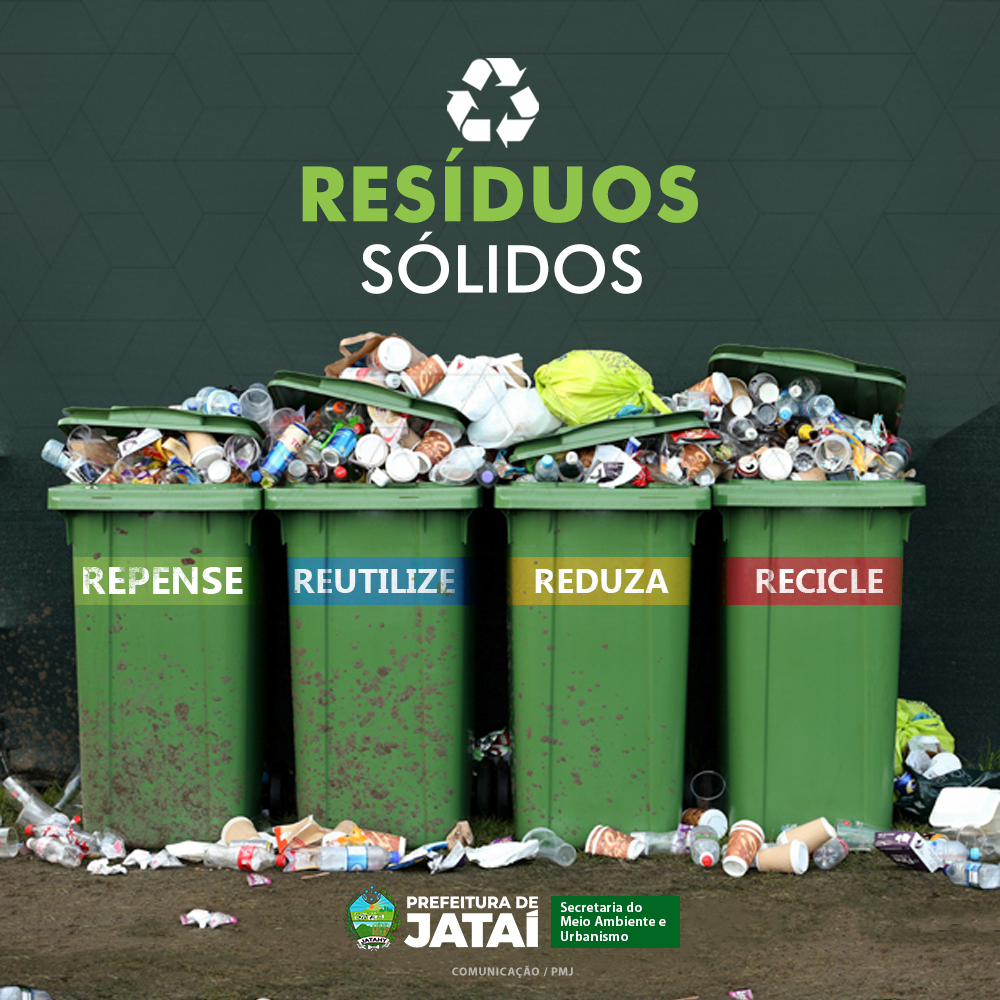
\includegraphics[width=5.90551in,height=5.90278in]{./imgSAEB_7_POR/media/image19.png}

\fonte{Ulysses Gusmão de Oliveira e Luiz Carlos Pereira Borges.
Prefeitura de Jatái. Separe seu lixo de forma adequada. 
Disponível em: https://www.jatai.go.gov.br/separe-seu-lixo-de-forma-adequada/.
Acesso em: 23 mai. 2023.}

Na imagem acima, pode-se perceber diversos recursos para que a mensagem
seja transmitida de maneira eficiente. No caso da escolha dos
verbos utilizados, é correto afirmar que:

\begin{escolha}

    \item as formas verbais no imperativo afirmativo sugerem ações.

    \item as formas verbais no infinitivo expressam instruções.

    \item as formas verbais no subjuntivo representam advertências.

    \item as formas verbais no infinitivo indicam ordens.

\end{escolha}

\coment{SAEB: Analisar os efeitos de sentido dos tempos, modos e/ou
vozes verbais com base no gênero textual e na intenção comunicativa.
 
a) Correta. O modo imperativo tem, de forma geral, a função de expressar
ordem, sugestão ou instrução. No caso específico do cartaz, sugere mudanças
de atitude por parte do leitor.
b) Incorreta. As formas verbais do cartaz não estão no infinitivo.
c) Incorreta. As formas verbais do cartaz não estão flexionadas no modo subjuntivo.
d) Incorreta. As formas verbais do cartaz não estão no infinitivo.}

\num{15} Observe a imagem a seguir para responder à questão.


\includegraphics[width=5.90551in,height=3.15278in]{./imgSAEB_7_POR/media/image20.png}

\fonte{Tribunal Regional Eleitoral de São Paulo. 
Tuitaço #RolêdasEleições alcança trending topics no Twitter.
Disponível em: https://www.tre-sp.jus.br/comunicacao/noticias/2022/Marco/tuitaco-roledaseleicoes-alcanca-trending-topics-no-twitter.
Acesso em: 22 mai. 2023.}

Pode-se afirmar que o público-alvo da campanha acima é

\begin{escolha}

    \item o público em geral, devido ao uso da linguagem formal combinada com imagens vivazes.
    
    \item o público adulto, daí a neutralidade sóbria do texto e a austeridade das imagens. 
    
    \item o público jovem, que se identificará com a imagem e que usa redes sociais.  
    
    \item a público infantil, pelo chamado lúdico do texto e das imagens à participação política. 

\end{escolha}

\coment{Avaliar a adequação das variedades linguísticas em contextos de uso.

a) Incorreta. A campanha é voltada ao público jovem: na imagem, é retratada 
uma adolescente, com a qual esse público se identifica; o texto de 
chamada contém uma hashtag, o que sugere uso das redes sociais, que é mais
recorrente entre os jovens.  
b) Incorreta. A campanha é voltada ao público jovem: na imagem, é retratada 
uma adolescente, com a qual esse público se identifica; o texto de 
chamada contém uma hashtag, o que sugere uso das redes sociais, que é mais
recorrente entre os jovens.  
c) Correta. A campanha é voltada ao público jovem: na imagem, é retratada 
uma adolescente, com a qual esse público se identifica; o texto de 
chamada contém uma hashtag, o que sugere uso das redes sociais, que é mais
recorrente entre os jovens.  
d) Incorreta. A campanha é voltada ao público jovem: na imagem, é retratada 
uma adolescente, com a qual esse público se identifica; o texto de 
chamada contém uma hashtag, o que sugere uso das redes sociais, que é mais
recorrente entre os jovens.}

\chapter{Simulado 2}
\markboth{Simulado 2}{}

\num{1} Leia o texto abaixo para responder à questão.

\begin{quote}

No período entre julho e setembro, a ocorrência de queimadas se torna
mais frequente, por conta da estiagem e da baixa umidade relativa do ar.
A Especialista CNN em agronegócio Carmen Perez falou sobre as técnicas
empregadas nas fazendas para evitar que o fogo se alastre e cause
destruição.

Ela explicou que a seca traz dois principais alertas para produtores
rurais: a necessidade de garantir alimento aos animais e a atenção ao
risco de queimadas.``Cada fazenda tem diversas estratégias para coibir e
enfrentar incêndios'', explicou. Dentre elas, estão os aceiros, áreas
livres em que circulam parte da plantação para interromper a propagação do
fogo, reservatórios de água estratégicos e equipamentos específicos.

``Estamos no início da seca, mas já estamos alertas para evitar
possíveis riscos para a natureza, plantações e animais'', disse Perez.

\end{quote}

\fonte{Fernanda Pinotti. CNN Brasil. Carmen Perez: Fazendas têm diversas 
estratégias para coibir incêndios. Disponível em:
https://www.cnnbrasil.com.br/economia/carmen-perez-fazendas-tem-diversas-estrategias-para-coibir-incendios/
Acesso em: 23 mai. 2023.}

Segundo a especialista em agronegócio, qual fator requer maior atenção
dos produtores rurais no que diz respeito ao risco de queimadas?

\begin{escolha}
    
    \item As altas temperaturas.
    
    \item O período de estiagem.
    
    \item A alimentação dos animais.
    
    \item O descaso com questões ambientais.

\end{escolha}

\coment{SAEB: Identificar teses, opiniões, posicionamentos explícitos e
argumentos em textos.  
a) Incorreta. Não há alusão ao aumento da temperatura como fator de risco.
b) Correta. Segundo a especialista, o período de estiagem e a baixa
umidade do ar são fatores de alerta para risco de queimadas.
c) Incorreta. Segundo a especialista, a seca traz duas preocupações para 
os produtores rurais: a necessidade de garantir alimento aos animais e a 
atenção ao risco de queimadas. A alimentação dos animais não é, portanto,
fator de risco de queimadas: é \textit{outra preocupação} dos produtores. 
d)Incorreta. No texto, não há alusão ao descaso com questões ambientais.}
  
\num{2} Leia o artigo 5 da Constituição Federal, de 1988, da República
Federativa do Brasil.

\begin{quote}

Art. 5º Todos são iguais perante a lei, sem distinção de qualquer
natureza, garantindo-se aos brasileiros e aos estrangeiros residentes no
País, a inviolabilidade do direito à vida, à liberdade, à igualdade, à
segurança e à propriedade.

\end{quote}

\fonte{Presidência da República. Constituição da República Federativa do Brasil 
de 1988. Disponível em: http://www.planalto.gov.br/ccivil_03/constituicao/constituicao.htm.
Acesso em: 23 mai. 2023.}

A divisão em artigos caracteriza o trecho como:

\begin{escolha}

    \item O texto de uma lei.

    \item Uma carta de solicitação.

    \item Uma reivindicação.

    \item Uma petição.

\end{escolha}

\coment{SAEB: Identificar formas de organização de textos normativos, legais e/ou reivindicatórios.

BNCC: EF69LP27 -- Analisar a forma composicional de textos pertencentes a
gêneros normativos/ jurídicos e a gêneros da esfera política, tais como
propostas, programas políticos (posicionamento quanto a diferentes ações
a serem propostas, objetivos, ações previstas etc.), propaganda política
(propostas e sua sustentação, posicionamento quanto a temas em
discussão) e textos reivindicatórios: cartas de reclamação, petição
(proposta, suas justificativas e ações a serem adotadas) e suas marcas
linguísticas, de forma a incrementar a compreensão de textos
pertencentes a esses gêneros e a possibilitar a produção de textos mais
adequados e/ou fundamentados quando isso for requerido

a) Correta. A divisão em artigos e parágrafos é uma característica
composicional de textos do gênero normativo/jurídico.
b) Incorreta. A divisão e forma composicional do trecho não correspondem
a cartas de solicitação.
c) Incorreta. A divisão e forma composicional do trecho não correspondem
a uma reivindicação.
d) Incorreta. A divisão e forma composicional do trecho não correspondem
a uma petição.} 

\num{3} Linguagem direta e curta, envolvendo poucos personagens, em espaço
delimitado e poucos conflitos e ações de personagens. Um texto que se
compõe de uma situação inicial, um conflito, clímax e desfecho. Estas
características estão presentes em:

\begin{escolha}

    \item Romance

    \item Contos

    \item Cartas pessoais

    \item Crônicas

\end{escolha}

\coment{SAEB: Analisar elementos constitutivos de textos pertencentes ao domínio
literário.

Bncc: EF69LP47 Analisar, em textos narrativos ficcionais, as diferentes
formas de composição próprias de cada gênero, os recursos coesivos que
constroem a passagem do tempo e articulam suas partes, a escolha lexical
típica de cada gênero para a caracterização dos cenários e dos
personagens e os efeitos de sentido decorrentes dos tempos verbais, dos
tipos de discurso, dos verbos de enunciação e das variedades
linguísticas (no discurso direto, se houver) empregados, identificando o
enredo e o foco narrativo e percebendo como se estrutura a narrativa nos
diferentes gêneros e os efeitos de sentido decorrentes do foco narrativo
típico de cada gênero, da caracterização dos espaços físico e
psicológico e dos tempos cronológico e psicológico, das diferentes vozes
no texto (do narrador, de personagens em discurso direto e indireto), do
uso de pontuação expressiva, palavras e expressões conotativas e
processos figurativos e do uso de recursos linguístico-gramaticais
próprios a cada gênero narrativo.

a) Incorreta. Os romances, embora apresentem algumas das
características elencadas no enunciado, em geral, são textos longos, 
com vários personagens que desenvolvem suas ações em vários cenários 
e conflitos.
b) Correta. As características elencadas no enunciado descrevem os 
contos.
c) Incorreta. Cartas pessoais possuem outras formas composicionais, tais
como saudação, corpo do texto e despedida.
d) Incorreta. As crônicas em geral possuem outras características tais
como temas do cotidiano e efeitos de humor.} 

\num{4} Leia o texto abaixo para responder à questão.

\begin{quote}

Uma pesquisa realizada pelo Instituto de Estudos em Saúde Coletiva
(Iesc) e pela Faculdade de Medicina (FM), atualmente em revisão na
revista Scientific Reports, indicou que os programas sociais de
transferência de renda foram essenciais durante o período crítico da
covid-19. A investigação também ressaltou que a população negra teve um
maior índice de mortalidade no mesmo recorte temporal.

O estudo, que analisou dados de contágio da doença colhidos entre março
de 2020 e setembro de 2021 em todo o Brasil, detectou uma relação
inversa entre as taxas de mortalidade e infecção e o número de pessoas
de uma mesma família que eram beneficiárias de algum dos programas
governamentais.

\end{quote}

\fonte{Carol Correia. Conexão UFRJ. Programas sociais foram fundamentais durante fase crítica da covid-19.
https://conexao.ufrj.br/2023/03/programas-sociais-foram-fundamentais-durante-fase-critica-da-covid-19/.
Acesso em: 24 mai 2023.}

No texto acima, a linguagem objetiva e a apresentação de dados de pesquisa são traços do 
gênero:

\begin{escolha}

    \item artístico-literário.

    \item de divulgação científica.

    \item jornalístico midiático.

    \item jurídico.

\end{escolha}

\coment{SAEB: Identificar elementos constitutivos de gêneros de divulgação
científica.

a) Incorreta. A linguagem objetiva e a apresentação de dados de pesquisa são 
traços do gênero de divulgação científica.
b) Correta.  Incorreta. A linguagem objetiva e a apresentação de dados de pesquisa são 
traços do gênero de divulgação científica.
c) Incorreta. A linguagem objetiva e a apresentação de dados de pesquisa são 
traços do gênero de divulgação científica.
d) Incorreta. A linguagem objetiva e a apresentação de dados de pesquisa são 
traços do gênero de divulgação científica.}

\num{5} Leia o texto abaixo para responder à questão. 

\begin{quote}

O livro \textit{A queda do Céu}, de Davi Kopenawa e Bruce Albert, é um modelo
inovador de produção textual, que combina a auto-etnografia de uma
cultura, o manifesto político das culturas tradicionais, os relatos de
vidas não ocidentais e uma visão cosmológica e espiritual do mundo,
quase extinta na sociedade moderna.

A obra retrata a vida do narrador (Kopenawa), desde sua iniciação
religiosa até alcançar o ápice como líder Yanomami.

Segundo sua cultura e tradições, os Yanomamis são os responsáveis por
assegurar que o céu não caia. Kopenawa, xamã da tribo, cita diversos
momentos em sua vida que exemplificam essas situações, onde ele ou os
antigos xamãs mobilizaram os espíritos para que a Floresta permanecesse
em equilíbrio.

\end{quote}

\fonte{Akil Alexandre Costa Silvério da Silva. Resenha do texto: \textit{A queda do Céu}: Davi Kopenawa e
Bruce Albert. Disponível em: https://edisciplinas.usp.br/pluginfile.php/3395103/mod_resource/content/1/T6\%20aperfei\%C3\%A7oado.pdf.
Acesso em: 24 mai. 2023.}

No texto acima, notam-se características da

\begin{escolha}

    \item crônica (temas do cotidiano de forma crítica e bem humorada).

    \item resenha crítica (características e explicações de outra obra).

    \item notícia (informações ao leitor sobre fatos ocorridos).

    \item peça de teatro (texto escrito para ser encenado). 

\end{escolha}

\coment{SAEB: Analisar elementos constitutivos de textos pertencentes ao 
domínioliterário.

a) Incorreta. O texto analisado apresenta características e explicações de outra obra.
b) Correta. O texto analisado apresenta características e explicações de outra obra.
c) Incorreta. O texto analisado apresenta características e explicações de outra obra.
d) Incorreta. O texto analisado apresenta características e explicações de outra obra.}

\num{6} Leia o texto abaixo para responder à questão. 

\begin{quote}

Na última década, o diabetes cresceu 54\% nos homens e 28,5\% nas
mulheres. Outra doença que tem crescido entre os brasileiros e que está
relacionada com o alto consumo de açúcar é a obesidade, que atinge
mais de 25\% da população adulta do país.

\end{quote}

\fonte{Ministério da Saúde. Saúde promove conscientização sobre o consumo de açúcar em webinário. 
Disponível em: https://aps.saude.gov.br/noticia/15359\#:~:text=Os\%20brasileiros\%20consomem\%2050\%25\%20a,adulto\%20\%C3\%A9\%20de\%2012\%20colheres.
Acesso em: 24 mai. 2023.}

De acordo com as informações acima, o consumo de açúcar pode ser
responsável pelos altos índices de obesidade. Além da obesidade, qual
outra doença pode estar relacionada ao consumo de açúcar? Assinale a
alternativa correta:

\begin{escolha}

  \item Diabetes.
  
  \item doenças crônicas não transmissíveis.
  
  \item doenças comuns em homens.
  
  \item doenças crônicas em mulheres. 

\end{escolha}

\coment{SAEB: Inferir informações implícitas em distintos textos.

a) Correta. O texto contém referências a apenas duas doenças relacionadas 
ao consumo de açúcar: diabetes e obesidade.
b) Incorreta. O texto contém referências a apenas duas doenças relacionadas 
ao consumo de açúcar: diabetes e obesidade.
c) Incorreta. O texto contém referências a apenas duas doenças relacionadas 
ao consumo de açúcar: diabetes e obesidade.
d) Incorreta. O texto contém referências a apenas duas doenças relacionadas 
ao consumo de açúcar: diabetes e obesidade.}


\num{7} Observe o meme abaixo para responder à questão.

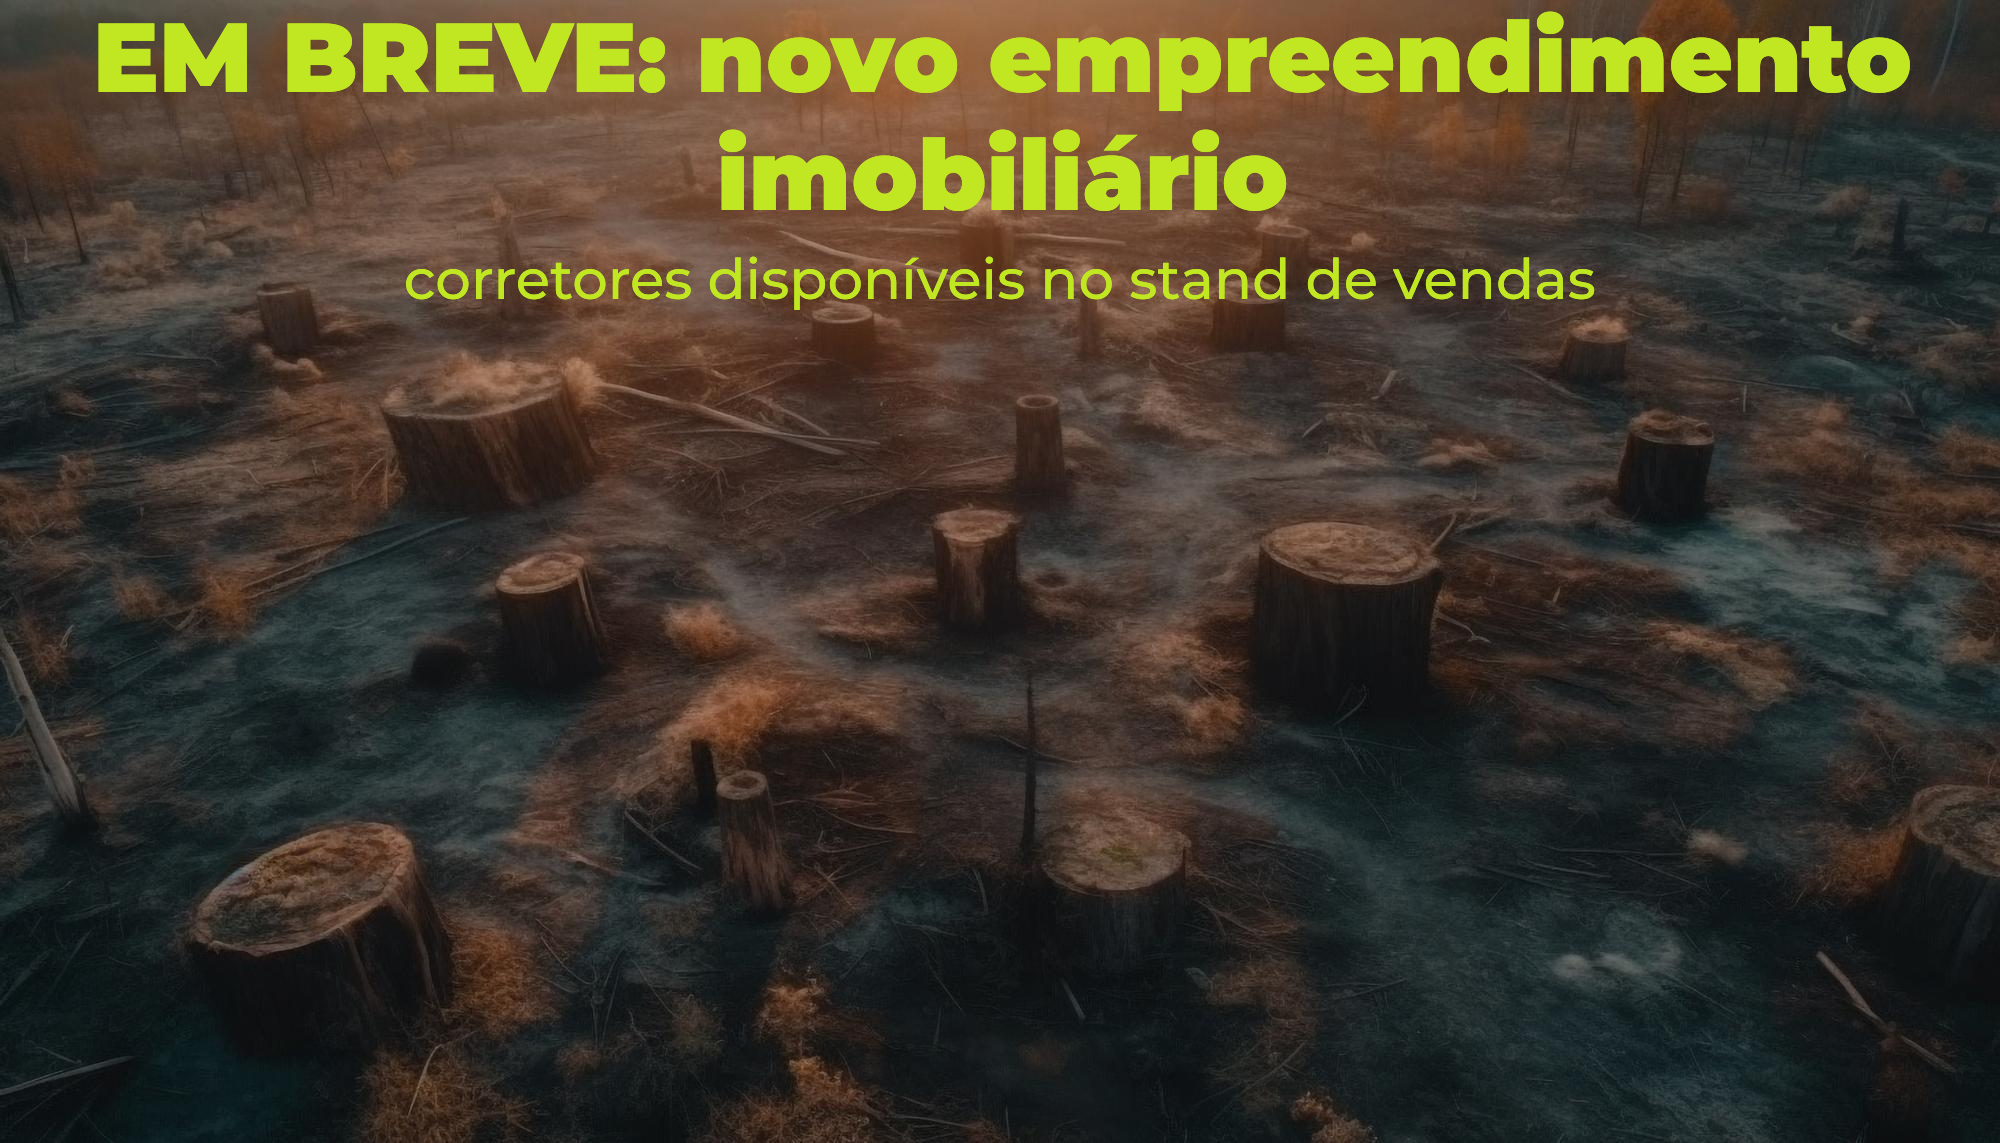
\includegraphics[width=4.16667in,height=3.03125in]{media/image21.png}

O efeito de sentido produzido pela imagem é bem claro. Assinale
alternativa que apresenta tais efeitos de sentido:

\begin{escolha}

    \item crítica ao desmatamento por meio de oposição.

    \item divulgação de informações por meio de imagem.

    \item persuasão por meio de frases injuntivas. 

    \item sensibilização por meio de frases motivacionais. 

\end{escolha}

\coment{SAEB: Inferir, em textos multissemiótico, efeitos de humor, ironia e/ou
crítica.

Bncc: EF69LP05 -- Inferir e justificar, em textos multissemióticos -- tirinhas, charges,
memes, gifs etc. --, o efeito de humor, ironia e/ou crítica pelo uso
ambíguo de palavras, expressões ou imagens ambíguas, de clichês, de
recursos iconográficos, de pontuação etc.

a) Correta. A crítica ao desmatamento se dá por meio da oposição entre o
desolamento causado pela destruição da natureza e o tom entusiástico da
propaganda do empreendimento imobiliário. 
b) Incorreta. O meme não contém divulgação de informações. 
c) Incorreta. O meme não contém frases injuntivas, isto é, imperativas.
d) Incorreta. O meme não contém frases motivacionais.} 

\num{8} Leia o texto abaixo para responder à questão. 

\begin{quote}

A teórica Kirin Narayan questiona esse dualismo e foca na qualidade das
relações que mantemos com as pessoas que buscamos representar em nossos
textos. Nesse sentido, a autora propõe desconstruir a ideia de que os
interlocutores poderiam ser classificados como meros indivíduos para
declarações acerca de um \textbf{``outro generalizado}'', impulsionando
assim um entendimento desses sujeitos como portadores de
\textbf{``vozes, perspectivas e dilemas''}.

\end{quote}

\fonte{Leonardo Bomfim. Desafios e potencialidades do ``pesquisador nativo'':
perspectivas etnográficas em um festival musical.
Disponível em: https://econtents.bc.unicamp.br/inpec/index.php/muspop/article/view/17627/12474.
Acesso em: 24 mai. 2023.}

Os termos destacados que aparecem entre aspas representam:

    \item as falas do autor sobre o tema.

    \item ideias que devem ser reforçadas.

    \item partes principais do argumento.

    \item citação das palavras de Kirin Naryan.

\end{escolha}

\coment{SAEB: Analisar efeitos de sentido produzido pelo uso de formas de
apropriação textual (paráfrase, citação etc.)

a) Incorreta. Os trechos entre aspas indicam citações das palavras da teórica Kirin Narayan.
b) Incorreta. Os trechos entre aspas indicam citações das palavras da teórica Kirin Narayan.
c) Incorreta. Os trechos entre aspas indicam citações das palavras da teórica Kirin Narayan.
d) Correta. Os trechos entre aspas indicam citações das palavras da teórica Kirin Narayan.}

\num{9} Leia o texto abaixo para responder à questão. 

\begin{quote}

Falando sobre o jogo Minecraft, Pedro Rezende se consolidou como o
maior YouTuber de games do Brasil. ``A ideia inicial começou quando eu
precisava de ajuda para passar de uma fase em um jogo e procurei na
internet''. A fala é de um dos maiores youtubers da atualidade no Brasil. O jovem
paranaense Pedro Rezende (19) mudou sua vida da água para o vinho depois
que abandonou a profissão de goleiro em um time de futebol na Itália
para seguir a carreira de youtuber de games por aqui.

\end{quote}

\fonte{Jadson Falcão. A União. Geração de youtubers faz sucesso entre o público jovem. 
Disponível em: https://auniao.pb.gov.br/noticias/caderno_diversidade/geracao-de-youtubers-faz-sucesso-entre-os-jovens-do-pais.
Acesso em: 24 mai. 2023.}

No contexto em que se insere, a expressão ``mudou sua vida da água para o vinho''
significa que 

\begin{escolha}

    \item a vida do garoto era miserável.

    \item o garoto trocou água por vinho.

    \item a vida do garoto continua a mesma.

    \item a vida do garoto mudou drasticamente.

\end{escolha}

\coment{SAEB: Analisar o uso de figuras de linguagem como estratégia
argumentativa.

a) Incorreta. No contexto em que se insere, a expressão significa que a vida 
do garoto mudou radicalmente. Não há elementos que indiquem que ele levava
uma vida miserável. 
b) Incorreta. No contexto em que se insere, a expressão significa que a vida 
do garoto mudou radicalmente.
c) Incorreta. No contexto em que se insere, a expressão significa que a vida 
do garoto mudou radicalmente.
d) Correta. No contexto em que se insere, a expressão significa que a vida 
do garoto mudou radicalmente.}

\num{10} Leia o texto abaixo para responder à questão.

\begin{quote}

\textbf{"Ariel, a Pequena Sereia" é opção de teatro para as crianças neste 
final de semana}

A programação cultural deste final de semana traz para o público infantil 
a peça teatral "Ariel, a Pequena Sereia". O espetáculo ganha sessões no Teatro 
Barreto Júnior, neste sábado (22) e domingo (23), às 16h30.

\end{quote}

\fonte{Folha de Pernambuco. 
Disponível em:
https://www.folhape.com.br/cultura/ariel-a-pequena-sereia-e-opcao-de-teatro-para-as-criancas-neste/267280/.
Acesso em: 24 mai. 2023}

Na manchete e no corpo do texto as aspas foram usadas para

\begin{escolha}
    
    \item citar a fala de um entrevistado.
    
    \item citar o nome de uma obra,
    
    \item citar uma gíria.
    
    \item dar ênfase ao termo.

\end{escolha}

\coment{SAEB: Analisar os efeitos de sentido decorrentes dos mecanismos de construção
de textos jornalísticos/midiáticos.

a) Incorreta. Na manchete e no corpo do texto as aspas foram usadas para citar o nome da peça.
b) Correta. Na manchete e no corpo do texto as aspas foram usadas para citar o nome da peça.
c) Incorreta. Na manchete e no corpo do texto as aspas foram usadas para citar o nome da peça.
d) Incorreta. Na manchete e no corpo do texto as aspas foram usadas para citar o nome da peça.}

\num{11} Leia os textos abaixo para responder à questão. 

\begin{quote}

\textbf{Texto 1}

Às 14h, ocorreu o acidente. Um desmoronamento interno fez com que uma
enorme rocha se desprendesse da montanha e caísse sobre o túnel,
fechando completamente a ligação com a superfície. Dentro da mina,
ficaram 33 mineiros -- 32 chilenos e 1 boliviano.

\end{quote}

\fonte{Rogério Simões. BBC News Brasil. 
Mineiros do Chile: a incrível e dramática saga acompanhada pelo mundo ao vivo na TV.
Disponível em: https://www.bbc.com/portuguese/internacional-55926799.
Acesso em: 24 mai. 2023.}

\textbf{Texto 2}

\begin{quote}

No dia 5 de agosto, um desmoronamento deixou 33 operários presos na mina
de San José, situada no deserto do Atacama, no Chile. Eles ficaram
incomunicáveis, a 700 metros de profundidade, durante 17 dias, até serem
descobertos pelas equipes de sondagem.

\end{quote}

\fonte{José Renato Salatiel. Mineiros do Chile: O resgate que emocionou o mundo.
Disponível em: https://vestibular.uol.com.br/resumo-das-disciplinas/atualidades/mineiros-do-chile-o-resgate-que-emocionou-o-mundo.htm.
Acesso em: 24 mai. 2023.}

Assinale a única afirmação comum aos dois textos. 

\begin{escolha}

    \item O acidente ocorreu às 14 horas.

    \item O acidente deixou 33 operários presos.

    \item Os mineiros ficaram presos por 17 dias.

    \item O acidente atingiu 32 chilenos e 1 boliviano.

\end{escolha}

\coment{Avaliar a fidedignidade de informações sobre um mesmo fato divulgado em
diferentes veículos e mídias.

a) Incorreta. A informação de que o acidente deixou 33 operários presos é a única comum aos dois textos.
b) Correta. A informação de que o acidente deixou 33 operários presos é a única comum aos dois textos.
c) Incorreta. A informação de que o acidente deixou 33 operários presos é a única comum aos dois textos.
d) Incorreta. A informação de que o acidente deixou 33 operários presos é a única comum aos dois textos.}

\num{12} Leia o texto abaixo para responder à questão. 

\begin{quote}

\textbf{Nordeste poderia crescer mais que o Brasil até 2030}

Combinar aumento da produtividade com redução das desigualdades seria a
melhor alternativa para elevar o PIB per capita na região.

\fonte{Instituto de Pesquisa Econômica Aplicada. Nordeste poderia crescer mais que o Brasil até 2030. 
Disponível em: 
https://www.ipea.gov.br/portal/categorias/45-todas-as-noticias/noticias/9506-nordeste-poderia-crescer-mais-que-o-brasil-ate-2030?highlight=WyJub3JkZXN0ZSIsIm5vcmRlc3RlJy4iXQ==.
Acesso em: 24 mai. 2023.}

De acordo com o texto, o Nordeste

\begin{escolha}
    
    \item vai crescer mais que o Brasil até 2030 e aumentar a produtividade para diminuir a desigualdade.
    
    \item só crescerá mais que o Brasil se combinar aumento da produtividade e redução da desigualdade. 
    
    \item já reduziu a desigualdade social e tem alcançado elevação proporcional do PIB.
    
    \item cresceu sensivelmente em relação ao Brasil, de modo que já conseguiu elevar o PIB.

\end{escolha}

\coment{SAEB: Identificar os recursos de modalização em textos diversos.

a) Incorreta. De acordo com o texto, o Nordeste crescerá mais do que o Brasil se combinar aumento
da produtividade com redução da desigualdade. 
b) Correta. De acordo com o texto, o Nordeste crescerá mais do que o Brasil se combinar aumento
da produtividade com redução da desigualdade. 
c) Incorreta. De acordo com o texto, o Nordeste crescerá mais do que o Brasil se combinar aumento
da produtividade com redução da desigualdade. 
d) Incorreta. De acordo com o texto, o Nordeste crescerá mais do que o Brasil se combinar aumento
da produtividade com redução da desigualdade.}

\num{13} Leia o texto abaixo para responder à questão. 

\begin{quote}

Sua história tem pouca coisa de notável. Fora Leonardo
algibebe em Lisboa, sua pátria; aborrecera-se porém do negócio,
e viera ao Brasil. Aqui chegando, não se sabe por proteção de
quem, alcançou o emprego de que o vemos empossado, e que
exercia, como dissemos, desde tempos remotos. Mas viera com
ele no mesmo navio, não sei fazer o quê, uma certa Maria da
Hortaliça, quitandeira das praças de Lisboa, saloia rechonchuda e
bonitota. O Leonardo, fazendo-se-lhe justiça, não era nesse tempo
de sua mocidade mal apessoado, e sobretudo era maganão. Ao
sair do Tejo, estando a Maria encostada à borda do navio, o
Leonardo fingiu que passava distraído por junto dela, e com o
ferrado sapatão assentou-lhe uma valente pisadela no pé direito.
A Maria, como se já esperasse por aquilo, sorriu-se como
envergonhada do gracejo, e deu-lhe também em ar de disfarce um
tremendo beliscão nas costas da mão esquerda. Era isto uma
declaração em forma, segundo os usos da terra: levaram o resto
do dia de namoro cerrado; ao anoitecer passou-se a mesma cena
de pisadela e beliscão, com a diferença de serem desta vez um
pouco mais fortes; e no dia seguinte estavam os dois amantes tão
eXtremosos e familiares, que pareciam sê-lo de muitos anos.

\end{quote}

\fonte{Manuel Antônio de Almeida. Memórias de um sargento de milícias.
Disponível em: https://digital.bbm.usp.br/handle/bbm/1601.
Acesso em: 24 mai. 2023.}

Assinale a alternativa correta no que se refere à coesão e à coerência 
do texto. 

\begin{escolha}

\item
  Em ``\textbf{Sua história} tem pouca coisa de notável'', o termo destacado
  se refere à história de Maria da Hortaliça.
\item
  Em ``assentou-\textbf{lhe} uma valente pisadela no pé direito'', o termo destacado
  se refere ao pé de Maria da Hortaliça.
\item
  Em ``deu-\textbf{lhe} também em ar de disfarce um tremendo beliscão'', o termo 
  destacado se refere ao pé de Maria da Hortaliça.
\item
  A expressão ``um pouco mais fortes'' refere-se à condição física de Leonardo e 
  Maria da Hortaliça.

\end{escolha}

\coment{SAEB: Analisar os processos de referenciação lexical e pronominal.

a) Incorreta.   Em ``\textbf{Sua história} tem pouca coisa de notável'', o termo destacado 
se refere à história de Leonardo.
a) Correta.   Em ``assentou-\textbf{lhe} uma valente pisadela no pé direito'', o termo destacado 
se refere ao pé de Maria da Hortaliça.
a) Incorreta.   Em ``deu-\textbf{lhe} também em ar de disfarce um tremendo beliscão'', o termo  
destacado se refere às costas da mão de Leonardo.
a) Incorreta.   A expressão ``um pouco mais fortes'' refere-se às ações de Leonardo e  
Maria da Hortaliça.}

\num{14} Leia o texto abaixo para responder à questão. 

\begin{quote}

A vacina salva vidas. Doenças que causavam milhares de vítimas no
passado, como varíola e poliomielite, foram erradicadas. Outras doenças
transmissíveis também deixaram de ser problema de saúde pública porque
foram eliminadas no Brasil e nas Américas, como o sarampo, rubéola e
rubéola congênita.

\end{quote}

\fonte{Ministério da Saúde. Programa Nacional de Imunizações -- Vacinação. Disponível em: https://www.gov.br/saude/pt-br/acesso-a-informacao/acoes-e-programas/programa-nacional-de-imunizacoes-vacinacao. Acesso em: 24 mai. 2023.}

Qual das seguintes opções melhor descreve a estratégia argumentativa
utilizada para enfatizar a importância da vacinação?

\begin{escolha}

    \item Emoção.
    
    \item Generalização.
    
    \item Lógica.
    
    \item Autoridade.

\end{escolha}

\coment{SAEB: Avaliar a eficácia das estratégias argumentativas em textos de
diferentes gêneros.

a) Incorreta. O autor não apela diretamente para as emoções do leitor,
mas para argumentos lógicos e fatos concretos.
b) Incorreta. O autor apresenta exemplos concretos de doenças
erradicadas e reduzidas graças à vacinação, sem generalizações.
c) Correta. O autor usa uma abordagem lógica para argumentar a favor da
vacinação, apresentando exemplos de doenças erradicadas e reduzidas
graças à vacinação, argumentando que a vacinação é estratégia mais
eficaz para prevenir doenças e salvar vidas.
d) Incorreta. O autor não se apoia em afirmações de especialistas para
argumentar a favor da vacinação.}

\num{15} Observe a imagem abaixo para responder à questão. 

\begin{quote}

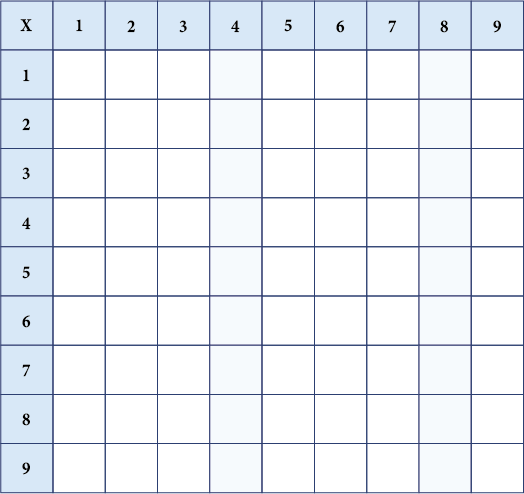
\includegraphics[width=5.90551in,height=3.18056in]{media/image22.png}

\fonte{https://www.tre-sp.jus.br/comunicacao/noticias/2022/Junho/campanha-201ctamo-junto201d-do-tre-sp-quer-incentivar-voto-consciente-dos-jovens.
Acesso em: 24 mai. 2023.}

A imagem acima faz parte de uma campanha incentivando a votação. Ao analisar
as escolhas de linguagem utilizadas podemos afirmar que a campanha se dirige: 

\begin{escolha}

    \item ao público idoso.

    \item ao público infantil.

    \item a mulheres.

    \item ao público jovem.

\end{escolha}

\coment{SAEB: Avaliar a adequação das variedades linguísticas em contextos de uso

a) Incorreta. O uso de recursos utilizados em redes sociais, como hashtags, 
não é o mais indicado ao público idoso.
b) Incorreta. O uso de gírias, símbolos e siglas de internet não é eficaz 
para o público infantil.
c) Incorreta. Não há nada na imagem que remeta ao público feminino.
d) Correta. O uso de gírias e hashtags utilizados no meio
digital é recurso eficaz para atingir o público jovem.}

\chapter{Simulado 3}
\markboth{Simulado 3}{}

\num{1} Leia o texto abaixo para responder à questão. 

\begin{quote}

\textbf{Alimentos que prejudicam o meio ambiente são também os piores à
saúde}

\textit{Comer cereais, frutas, verduras, batatas e azeite de oliva protege o
planeta e previne doenças}

Aproximadamente 60\% dos fatores de risco responsáveis por todas as
doenças são o resultado de uma dieta de má qualidade. Esse fato está
ligado à saúde do planeta. Um estudo publicado na revista PNAS demonstra
que os alimentos mais prejudiciais ao ser humano também o são para a
Terra.

Os pesquisadores analisaram 15 alimentos que fazem parte da dieta diária
ocidental. Ligaram a maneira como são produzidos (a água que se gasta, a
superfície implicada e os produtos químicos utilizados, entre outros)
aos resultados de estudos anteriores sobre o impacto desses mesmos
alimentos sobre a saúde. E tudo se encaixava. As frutas, verduras, a
batata, o azeite de oliva, os legumes, as frutas secas e os cereais são
os alimentos mais saudáveis e que, além disso, têm impacto mínimo sobre
o planeta.

A carne vermelha processada e não processada, por outro lado, é um
produto que deveria sair da lista de compras.

O peixe é um dilema. É uma opção saudável, como a maioria das pessoas
sabe, mas tem uma pegada ambiental maior, ao lado do frango e dos
laticínios, do que as dietas baseadas em vegetais, de acordo com os
resultados do estudo. Basulto afirma que um produto é benéfico quando
impede o consumidor de comer alimentos mais prejudiciais para sua saúde.
``Se o cliente come peixe e não consome carne vermelha, portanto, é bom
para ele e para o planeta'', acrescenta.

\fonte{Agathe Cortes. El País Brasil. 
Disponível em: https://brasil.elpais.com/brasil/2019/10/29/ciencia/1572344750_688431.html.
Acesso em: 22 mai. 2023.}

Segundo a reportagem, assinale a alternativa que contém os alimentos
mais saudáveis e que menos impactam o planeta:

\begin{escolha}
  
    \item cereais, ovos, legumes.
  
    \item frutas, verduras, cereais.
  
    \item frutas, verduras, frango.
  
    \item frutas secas, azeite, carnes.

\end{escolha}

\coment{SAEB: Identificar teses, opiniões, posicionamentos explícitos e
argumentos em textos.

a) Incorreta. A reportagem não cita os ovos.
b)Correta. Estes estão entre os alimentos mais saudáveis e de menor
impacto junto com azeite e frutas secas.
c) Incorreta. Segundo o texto, o consumo de frango tem ``pegada ambiental
maior''.
d) Incorreta. As carnes, segundo a reportagem, deveriam ser retiradas
da dieta.}

\num{2} Leia o texto abaixo para responder à questão. 

\begin{quote}

No caso, a quantidade de comida industrializada ingerida parece
influenciar no aparecimento de doenças e na quantidade de mortes
prematuras. Esses estudos, no entanto, não conseguem demonstrar qual
seria o mecanismo por trás dessa aparente correlação.

A geriatra Claudia Suemoto, da Faculdade de Medicina da USP, que
coordenou o estudo do Elsa sobre ultraprocessados e desempenho
cognitivo, espera superar essa limitação em breve. Serão feitas imagens
do cérebro de voluntários para ver se o alto consumo de ultraprocessados
pode causar eventos isquêmicos ou pequenos derrames cerebrais, que, ao
longo do tempo, poderiam comprometer as funções cognitivas. ``Dessa
forma, poderemos investigar possíveis mecanismos que expliquem a
associação do ponto de vista estrutural'', conta Suemoto.

\end{quote}

Segundo o texto, a limitação a ser superada pela pesquisa é:

\begin{escolha}

    \item diminuir a quantidade de ingestão de ultraprocessados para evitar derrames e melhorar o desempenho cognitivo.

    \item impossibilidade de demonstrar o mecanismo por trás da relação entre o consumo de ultraprocessados e as mortes prematuras.
  
    \item conseguir imagens do cérebro de voluntários que sofreram derrame cerebral causado pelo consumo excessivo de ultraprocessados.
  
    \item estudar as funções cognitivas e os eventos isquêmicos de quem sofreu derrame cerebral causado pelo consumo excessivo de ultraprocessados.

\end{escolha}

\coment{SAEB: Identificar elementos constitutivos de gêneros de divulgação científica.

a) Incorreta. Como se observa no primeiro parágrafo, impossibilidade de demonstrar o mecanismo por trás da relação entre o consumo de ultraprocessados e as mortes prematuras.
b) Correta. Como se observa no primeiro parágrafo, impossibilidade de demonstrar o mecanismo por trás da relação entre o consumo de ultraprocessados e as mortes prematuras.
c) Incorreta. Como se observa no primeiro parágrafo, impossibilidade de demonstrar o mecanismo por trás da relação entre o consumo de ultraprocessados e as mortes prematuras.
d) Incorreta. Como se observa no primeiro parágrafo, impossibilidade de demonstrar o mecanismo por trás da relação entre o consumo de ultraprocessados e as mortes prematuras.}

\num{3} Leia o texto abaixo para responder à questão. 

\begin{quote}

\textbf{Título I}

Das Disposições Preliminares

Art. 1º Esta Lei dispõe sobre a proteção integral à criança e ao
adolescente.

Art. 2º Considera-se criança, para os efeitos desta Lei, a pessoa até
doze anos de idade incompletos, e adolescente aquela entre doze e
dezoito anos de idade.

Parágrafo único. Nos casos expressos em lei, aplica-se excepcionalmente
este Estatuto às pessoas entre dezoito e vinte e um anos de idade.

\end{quote}

\fonte{Presidência da República. 
Disponível em: https://www.planalto.gov.br/ccivil_03/leis/l8069.htm.
Acesso em: 24 mai. 2023.}

Estão presentes no texto acima e são características de textos legais ou
jurídicos

\begin{escolha}

\item linguagem impessoal e organização em títulos, capítulos e sessões.
\item uso de linguagem informal e organização em parágrafos e estrofes.
\item linguagem rebuscada e organização em títulos e subtítulos.
\item uso da primeira pessoa e organização em livre.
\end{escolha}

\coment{SAEB:  Identificar formas de organização de textos normativos, legais
e/ou reivindicatórios.

BNCC: EF69LP20 -- Identificar, tendo em vista o contexto de produção, a
forma de organização dos textos normativos e legais, a lógica de
hierarquização de seus itens e subitens e suas partes: parte inicial
(título -- nome e data -- e ementa), blocos de artigos (parte, livro,
capítulo, seção, subseção), artigos (caput e parágrafos e incisos) e
parte final (disposições pertinentes à sua implementação) e analisar
efeitos de sentido causados pelo uso de vocabulário técnico, pelo uso do
imperativo, de palavras e expressões que indicam circunstâncias, como
advérbios e locuções adverbiais, de palavras que indicam generalidade,
como alguns pronomes indefinidos, de forma a poder compreender o caráter
imperativo, coercitivo e generalista das leis e de outras formas de
regulamentação.

a) Incorreta. O texto se caracteriza pela linguagem impessoal e organização em 
títulos, capítulos e sessões.
b) Correta. O texto se caracteriza pela linguagem impessoal e organização em 
títulos, capítulos e sessões. 
c) Incorreta. O texto se caracteriza pela linguagem impessoal e organização em 
títulos, capítulos e sessões. 
d) Incorreta. O texto se caracteriza pela linguagem impessoal e organização em 
títulos, capítulos e sessões.} 

\num{4} Leia o texto abaixo para responder à questão. 

\begin{quote}

\textbf{Faciap promove encontros para jovens empreendedores em Curitiba}

Entre quinta (25) e sexta-feira (26) acontecem dois eventos promovidos
pelos integrantes da ala jovem da Federação das Associações Comerciais e
Empresariais do Paraná (Faciap).

A Assembleia Geral Ordinária (AGO) da Confederação Nacional de Jovens
Empresários (Conaje), que começa nesta quinta-feira (25) é um evento
nacional e vai reunir jovens empreendedores de todo o Brasil. Já na
sexta-feira (26) acontece o Encontro Paranaense de Jovens
Empreendedores.

\end{quote}

\fonte{CBN Curitiba. Faciap promove encontros para jovens empreendedores 
em Curitiba.
Disponível em: https://cbncuritiba.com.br/materias/faciap-promove-encontros-para-jovens-empreendedores-em-curitiba/.
Acesso em: 24 mai. 2023.}

Considerando os elementos constitutivos dos textos jornalísticos, a
informação sobre a cidade onde ocorre o evento está localizada:

\begin{escolha}
  
  \item no corpo da notícia.
  
  \item na lide.
  
  \item no título auxiliar.
  
  \item na manchete.

\end{escolha}

\coment{Identificar elementos constitutivos de textos pertencentes ao domínio
jornalístico/midiático.

a) Incorreta. A informação sobre Curitiba está localizada na manchete.
b) Incorreta. A informação sobre Curitiba está localizada na manchete.
c) Incorreta. A informação sobre Curitiba está localizada na manchete.
d) Correta. A informação sobre Curitiba está localizada na manchete.}

\num{5} Leia o poema abaixo para responder à questão. 

\begin{quote}
\begin{verse}

Mas a minha tristeza é sossego \\
Porque é natural e justa \\
E é o que deve estar na alma \\
Quando já pensa que existe \\
E as mãos colhem flores sem ela dar por isso.

\end{verse}
\end{quote}

\fonte{Alberto Caeiro (heterônimo de Fernando Pessoa. O Guardador de Rebanhos. 
Disponível em: http://www.dominiopublico.gov.br/download/texto/pe000001.pdf.
Acesso em: 24 mai. 2023.}

Pode-se inferir que, para o eu lírico do poema, sua tristeza

\begin{escolha}

    \item causa confusão ao colher as flores.

    \item impede que a justiça natural ocorra.

    \item repousa distante dele mesmo. 

    \item traz quietude por ser natual e justa. 

\end{escolha}

\coment{SAEB: Inferir informações implícitas em distintos textos.

a) Incorreta. Para o eu lírico, sua tristeza é sossego, sem causa confusão.
b) Incorreta. Para o eu lírico, sua tristeza é natural e justa. 
c) Incorreta. Para o eu lírico, sua tristeza está na alma.
d) Correta. Para o eu lírico, sua tristeza é sossego (portanto, quietude),
por ser natural e justa.}

\num{6} Leia o texto abaixo para responder à questão. 

%Excluí essa imagem
%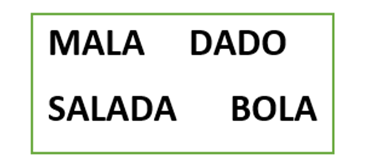
\includegraphics[width=5.90551in,height=1.70833in]{media/image3.png}
%\fonte{https://tirasarmandinho.tumblr.com/}{{https://tirasarmandinho.tumblr.com/}}.
%Acesso em 26 de Abr de 2023

\begin{quote}

Dito isto, expirei às duas horas da tarde de uma
sexta-feira do mês de agosto de 1869, na minha bela
chácara de Catumbi. Tinha uns sessenta e quatro anos,
rijos e prósperos, era solteiro, possuía cerca de trezentos
contos e fui acompanhado ao cemitério por onze amigos.
Onze amigos! Verdade é que não houve cartas nem
anúncios. Acresce que chovia -- peneirava uma chuvinha
miúda, triste e constante, tão constante e tão triste \ldots{}

\end{quote}

\fonte{Machado de Assis. Memórias Póstumas de Brás Cubas. 
Disponível em: https://digital.bbm.usp.br/handle/bbm/4826.
Acesso em: 24 mai. 2023.}

Nos dois últimos períodos do parágrafo, o narrador pretende 

\begin{escolha}

    \item justificar o pequeno número de presentes a seu enterro. 

    \item lamentar a injustiça de ter morrido cedo e com saúde.

    \item exaltar a popularidade que tinha entre os amigos.

    \item agradecer sinceramente aos amigos que o acompanharam.

\end{escolha}

\coment{Saeb: Analisar elementos constitutivos de textos pertencentes ao domínio literário.

a) Correta. Os dois últimos períodos do parágrafo pretendem justificar a baixa
adesão, de apenas onze amigos, ao enterro do narrador. Note-se: ao iniciar o 
penúltimo período com ``verdade é que'' ele pretende explicar por que tão 
poucas pessoas compareceram: porque não houve anúncio de sua morte e porque chovia.
b) Incorreta. Os dois últimos períodos do parágrafo pretendem justificar a baixa
adesão, de apenas onze amigos, ao enterro do narrador. Note-se: ao iniciar o 
penúltimo período com ``verdade é que'' ele pretende explicar por que tão 
poucas pessoas compareceram: porque não houve anúncio de sua morte e porque chovia.
c) Incorreta. Os dois últimos períodos do parágrafo pretendem justificar a baixa
adesão, de apenas onze amigos, ao enterro do narrador. Note-se: ao iniciar o 
penúltimo período com ``verdade é que'' ele pretende explicar por que tão 
poucas pessoas compareceram: porque não houve anúncio de sua morte e porque chovia.
d) Correta. Os dois últimos períodos do parágrafo pretendem justificar a baixa
adesão, de apenas onze amigos, ao enterro do narrador. Note-se: ao iniciar o 
penúltimo período com ``verdade é que'' ele pretende explicar por que tão 
poucas pessoas compareceram: porque não houve anúncio de sua morte e porque chovia.}

\num{7} Leia os textos abaixo para responder à questão. 

\textbf{Exemplo 1}

\begin{quote}

\textit{Câncer de mama}
É o tipo de câncer mais frequente na mulher brasileira. Nesta doença,
ocorre um desenvolvimento anormal das células da mama, que
multiplicam-se repetidamente até formarem um tumor maligno.

\textit{Como descobrir a doença mais cedo?}
Toda mulher com 40 anos ou mais de idade deve procurar um ambulatório,
centro ou posto de saúde para realizar o exame clínico das mamas
anualmente, além disso, toda mulher, entre 50 e 69 anos deve fazer pelo
menos uma mamografia a cada dois anos. O serviço de saúde deve ser
procurado mesmo que não tenha sintomas!

\textit{O que é o exame clínico das mamas?}
É o exame das mamas realizado por médico ou enfermeiro treinado para
essa atividade. Neste exame poderão ser identificadas alterações nas
mesmas. Se for necessário, será indicado um exame mais específico, como
a mamografia.

\textit{O auto-exame previne a doença?}
O exame das mamas realizado pela própria mulher, apalpando os seios,
ajuda no conhecimento do próprio corpo, entretanto, esse exame não
substitui o exame clínico das mamas realizado por um profissional de
saúde treinado. Caso a mulher observe alguma alteração deve procurar
imediatamente o serviço de saúde mais próximo de sua residência. Mesmo
que não encontre nenhuma alteração no auto-exame, as mamas devem ser
examinadas uma vez por ano por um profissional de saúde!

\end{quote}

\fonte{Biblioteca Virtual em Saúde. Câncer de mama. Disponível em:
https://bvsms.saude.gov.br/cancer-de-mama/.
Acesso em: 24 mai. 2023.}

\textbf{Exemplo 2}

\begin{quote}

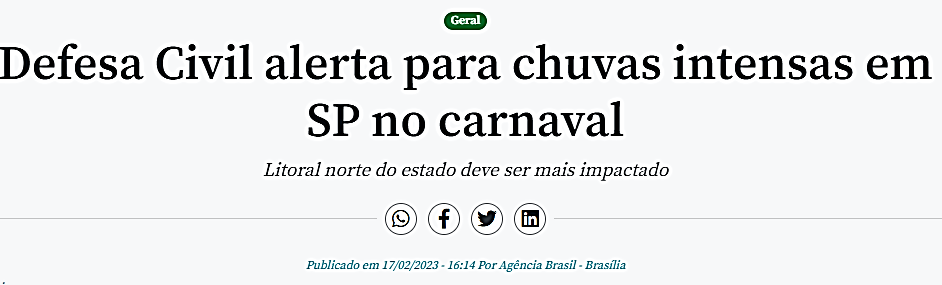
\includegraphics[width=3.73839in,height=3.73839in]{media/image4.png}

\end{quote}

\fonte{Ministério da Gestão e da Inovação em Serviços Públicos. 
Câncer de mama: é hora de falar sobre isso. 
Disponbível em: https://www.gov.br/arquivonacional/pt-br/canais_atendimento/imprensa/copy_of_noticias/cancer-de-mama-e-hora-de-falar-sobre-isso.
Acesso em: 24 mai. 2023.}

Os dois exemplos trazem informações sobre o câncer de mama e os exames
necessários para detectar a doença. Nos dois casos, o que faz com que as
informações sejam confiáveis é a presença de

\begin{escolha}
    
    \item textos explicativos.
    
    \item imagens e textos.
    
    \item citação de fontes oficiais.
    
    \item linguagem clara.

\end{escolha}

\coment{SAEB: Avaliar a fidedignidade de informações sobre um mesmo fato
divulgado em diferentes veículos e mídias.

a) Incorreta. Embora os textos sejam bastante explicativos, este não é
um critério de confiabilidade.
b) Incorreta. As figuras e textos só aparecem no Exemplo 2 e não podem
ser considerados recursos para avaliar a confiabilidade das informações.
c) Correta. Em ambos os casos a fonte das informações é o INCA, órgão
oficial que trata das questões relativas ao câncer de mama e demais
formas da doença. 
d) Incorreta. Embora a linguagem utilizada seja clara, este não é um
critério de confiabilidade.}

\num{8} Leia o texto abaixo para responder à questão. 

\begin{quote}

\textbf{O que a ciência diz sobre os remédios naturais para dormir}

\textit{Se você tomar um chazinho à base de ervas ou borrifar o quarto com
aromas agradáveis... será que vai conseguir dormir como um bebê?}

O sono raramente é mais desejado do que quando não conseguimos dormir.

E há uma grande variedade de remédios caseiros que prometem nos ajudar a
pegar no sono sem recorrer a produtos farmacêuticos.

\end{quote}

\fonte{G1. Disponível em: https://g1.globo.com/saude/noticia/2023/04/26/o-que-a-ciencia-diz-sobre-os-remedios-naturais-para-dormir.ghtml. 
Acesso em: 24 mai. 2023.}

A expressão ``raramente'', para se referir ao desejo de dormir, expressa:

\begin{escolha}
  
  \item que o sono é mais desejado quando não se consegue dormir.
  
  \item que na maioria das vezes o sono é desejado em qualquer ocasião.
  
  \item que sempre sentimos sono quando precisamos dormir.
  
  \item que só sentimos sono quando não desejamos dormir. 

\end{escolha}

\coment{SAEB: Analisar os efeitos de sentido produzidos pelo uso de modalizadores em
textos diversos.

a) Correta. A explicação desta alternativa corresponde às afirmações contidas
em ``O sono raramente é mais desejado do que quando não conseguimos dormir''.
b) Incorreta.A explicação desta alternativa não corresponde às afirmações contidas
em ``O sono raramente é mais desejado do que quando não conseguimos dormir''.
c) Incorreta.A explicação desta alternativa não corresponde às afirmações contidas
em ``O sono raramente é mais desejado do que quando não conseguimos dormir''.
d) Incorreta.A explicação desta alternativa não corresponde às afirmações contidas
em ``O sono raramente é mais desejado do que quando não conseguimos dormir''.}

\num{9} Leia o texto abaixo para responder à questão. 

\begin{quote}

\textbf{-- Por que não ser também um chato?}

\begin{verse}

Mas de repente percebi \\
Sem ser doutor \\
Que a chatice é a única doença \\
que não dói no portador \\
E resolvi ser chato. 

\end{verse}
\end{quote}

\fonte{Millor Fernandes. Poeminha Maçante, no livro Circo de palavras: histórias, poemas, pensamentos.
São Paulo: Ática, 2007. p. 63.}

Segundo o poema, o eu lírico escolheur ser chato porque 

\begin{escolha}

  \item a chatice é uma doença.
  
  \item ser chato não dói.
  
  \item ele queria ser doutor.
  
  \item se percebeu chato de repente.

\end{escolha}

\coment{SAEB: Avaliar a eficácia das estratégias argumentativas em textos de
diferentes gêneros.

a) Incorreta. O eu lírico escolheu ser chato porque ``a chatice é a única doença / 
que não dói no portador''. 
b) Correta. O eu lírico escolheu ser chato porque ``a chatice é a única doença / 
que não dói no portador''. 
c) Incorreta. O eu lírico escolheu ser chato porque ``a chatice é a única doença / 
que não dói no portador''. 
chatice é uma doença=
d) Incorreta. O eu lírico escolheu ser chato porque ``a chatice é a única doença / 
que não dói no portador''.} 

\num{10} Leia o texto abaixo para responder à questão. 

\begin{quote}

O casamento fez-se onze meses depois, e foi a mais bela festa das
relações dos noivos. Amigas de Clara, menos por amizade que por
inveja, tentaram arredá-la do passo que ia dar. Não negavam a gentileza
do noivo, nem o amor que lhe tinha, nem ainda algumas virtudes; diziam
que era dado em demasia a patuscadas.

\end{quote}

\fonte{Machado de Assis. Pai contra mãe. 
Disponível em: http://www.dominiopublico.gov.br/download/texto/bv000245.pdf.
Acesso em: 24 mai. 2023.}

De acordo com o texto, as amigas de Clara

\begin{escolha}

    \item tentaram impedir o casamento dela porque lhe nutriam amizade honesta.

    \item persuadiram-na a desistir por causa da falsidade dos sentimentos do noivo.  

    \item desaprovavam o casamento porque não lhe nutriam amizade verdadeira.

    \item tentaram convencê-la a desistir do casamento por inveja, apesar da amizade.

\end{escolha}

\coment{SAEB: Analisar os processos de referenciação lexical e pronominal.

a) Incorreta. As amigas de Clara eram evidentemente mais invejosas do que amigas, 
como se verifica na expressão ``menos por amizade que por inveja''.
b) Incorreta. Os sentimentos do noivo não são questionados. As amigas de Clara, 
invejosas, dizem-lhe que ele, embora apaixonado e virtuoso, era festeiro demais.
c) Incorreta. Embora invejosas, as amigas de Clara tinham-lhe alguma amizade.
d) Correta. A chave para escolher esta alternativa é compreender que, por meio da  
expressão ``menos por amizade que por inveja'' o narrador evidencia que, por mais 
houvesse amizade entre Clara e as amigas, estas tentaram convencê-la a desistir 
do casamento por inveja.} 

\num{11} Observe os períodos a seguir.

\begin{itemize}

    \item \textbf{Já que} o vento soprava muito forte, decidiram não sair
naquela noite.

    \item Eu não consegui ir ao escritório \textbf{porque} estava muito doente

    \item Os jovens terão suas necessidades ouvidas, \textbf{exceto} se se
afastarem dos responsáveis.

    \item \textbf{Embora} estivesse triste, não chorou.

\end{itemize}

Assinale a alternativa que indica corretamente as relações de sentido
expressas pelos conectivos em destaque.

\begin{escolha}

    \item causa, causa, condição, concessão.

    \item comparação, condição, finalidade, oposição.

    \item causa, oposição, condição, finalidade

    \item finalidade, comparação, tempo, causa.

\end{escolha}

\coment{SAEB: Analisar os mecanismos que contribuem para a progressão textual.

a) Correta. Na primeira afirmação, a causa da decisão de não sair é o vento soprar forte;
na segunda, estar doente é a causa da impossibilidade de ir ao escritório; na terceira, 
as necessidades dos jovens só não serão ouvidas em uma condição: se eles se afastarem dos
responsáveis; na última, apesar da tristeza, não houve lágrimas. 
b) Incorreta. Na primeira afirmação, a causa da decisão de não sair é o vento soprar forte;
na segunda, estar doente é a causa da impossibilidade de ir ao escritório; na terceira, 
as necessidades dos jovens só não serão ouvidas em uma condição: se eles se afastarem dos
responsáveis; na última, apesar da tristeza, não houve lágrimas.  
c) Incorreta. Na primeira afirmação, a causa da decisão de não sair é o vento soprar forte;
na segunda, estar doente é a causa da impossibilidade de ir ao escritório; na terceira, 
as necessidades dos jovens só não serão ouvidas em uma condição: se eles se afastarem dos
responsáveis; na última, apesar da tristeza, não houve lágrimas. 
d) Incorreta. Na primeira afirmação, a causa da decisão de não sair é o vento soprar forte;
na segunda, estar doente é a causa da impossibilidade de ir ao escritório; na terceira, 
as necessidades dos jovens só não serão ouvidas em uma condição: se eles se afastarem dos
responsáveis; na última, apesar da tristeza, não houve lágrimas.}  

\num{12} Leia o texto abaixo para responder à questão. 

\begin{quote}

Em relação ao consumo de agrotóxicos no Brasil, hoje paira uma grande
incerteza sobre os números exatos. No ano de 2015, só foram divulgados
os valores em dólares dos ganhos da indústria. Neste sentido, houve uma
forte queda, de 21\%, em relação a 2014. No entanto, se considerarmos a
variação do câmbio, vemos que na verdade o faturamento em reais subiu de
R\$28 para R\$32 bilhões. Como uma boa parte do custo dos agrotóxicos é
importada, não é possível saber se aumentou ou diminuiu a quantidade de
agrotóxicos em 2015.

\end{quote}

\fonte{Alan Tygel. Agrotóxicos no Brasil: O veneno ainda está na mesa.  
Disponível em:
https://www.brasildefato.com.br/2016/11/23/agrotoxicos-no-brasil-o-veneno-ainda-esta-na-mesa.
Acesso em: 24 mai. 2023.}

Assinale a alternativa que contém a figura de linguagem correta e o
trecho em que essa figura aparece.

\begin{escolha}

    \item Hipérbole em ``Agrotóxicos do Brasil''. 

    \item Metáfora em ``hoje paira uma grande incerteza sobre os números exatos''. 

    \item Metonímia em ``O veneno ainda está na mesa''. 

    \item Hipérbole em ``Neste sentido, houve uma forte queda, de 21\%''. 

\end{escolha}

\coment{SAEB: Analisar o uso de figuras de linguagem como estratégia argumentativa.

a) Incorreta. Não ocorre metáfora na expressão indicada.
b) Incorreta. Não ocorre metáfora na expressão indicada.
c) Correta. Ocorre metonímia no uso do termo ``o veneno'' para se
referir à alimentação contaminada por agrotóxicos. 
d) Incorreta. Não ocorre hipérbole na expressão indicada.}

\num{13} Leia o texto abaixo para responder à questão. 

\begin{quote}

Uma noite destas, vindo da cidade para o Engenho
Novo, encontrei no trem da Central um rapaz aqui do
bairro, que eu conheço de vista e de chapéu. 
Cumprimentou-me, sentou-se ao pé de mim, falou da lua
e dos ministros, e acabou recitando-me versos. A viagem 
era curta, e os versos \textbf{pode ser que não fossem} 
inteiramente maus. Sucedeu, porém, que, como eu estava 
cansado, fechei os olhos três ou quatro vezes; tanto 
bastou para que ele interrompesse a leitura e metesse 
os versos no bolso.

\end{quote}

\fonte{Machado de Assis. Dom Casmurro. 
Disponível em: https://www.ic.unicamp.br/~stolfi/misc/2012-02-13-domine-casmurrus.pdf.
Acesso em: 24 mai. 2023.}

A escolha dos verbos no trecho em destaque dá a entender que o narrador

\begin{escolha}

  \item julga ruins os versos do rapaz e interrompe-lhe a leitura.

  \item considera bons os versos do rapaz, apesar de cansativos.

  \item não tolera a falta de qualidade da poesia do rapaz.

  \item avalia que os versos não eram ruins, sem considerá-los bons.

\end{escolha}

\coment{SAEB: Analisar os efeitos de sentido dos tempos, modos e/ou vozes verbais com
base no gênero textual e na intenção comunicativa.

a) Incorreta. O narrador não deixa claro que considerava os versos ruins, como se
pode verificar pela escolha das formas verbais destacadas no texto.
b) Incorreta. O narrador não deixa claro que considera bons os versos do rapaz,como se
pode verificar pela escolha das formas verbais destacadas no texto.
c) Incorreta. A escolha das formas verbais destacadas no texto não permite fazer uma
afirmação tão categórica quanto a desta alternativa.
d) Correta. A escolha das formas verbais destacadas no texto sugere que os versos do
rapaz, embora não pudessem ser chamados de completamente ruins, também não poderiam
ser chamados de bons.}

\num{14} Leia o texto abaixo para responder à questão. 

\begin{quote}

\textbf{Os cosplays mais irados de 2021}

Apesar da pandemia, a criatividade na cultura pop não parou,
por isso vamos ver os cosplays que mais se destacaram em 2021 até
agora!

\end{quote}

\fonte{Terra. Os cosplays mais irados de 2021. 
Disponível em: https://www.terra.com.br/gameon/geek/os-cosplays-mais-irados-de-2021,b409f1697bb7db34500d0614340e6423966k7p1p.html.
Acesso em: 24 mai. 2023.}

No exemplo acima, observam-se algumas variações linguísticas. Assinale a
alternativa que contém a correta descrição de termos do texto.

\begin{escolha}
  
  \item cosplays: estrangeirismo.
  
  \item cultura pop: regionalismo.
  
  \item irados: norma-padrão.
  
  \item criatividade: gíria.

\end{escolha}

\coment{SAEB: Analisar as variedades linguísticas em textos.

a) Correta. O termo ``cosplay'' vem do inglês.
b) Incorreta. A expressão ``'cultura pop'' é amplamente utilizada nas mídias,
sem se restringir a uma região específica.
c) Incorreta. ``Irado'', no contexto, é gíria. 
d) Incorreta. O substantivo ``criatividade'' não é gíria.} 

\num{15} Leia o texto abaixo para responder à questão. 

\begin{quote}

\textbf{Os ``causos'' de Joseli Dias}

O ofício de jornalista de Joseli Dias deu-lhe a agilidade de lidar com
as palavras. As narrativas das lendas e dos ``causos'' desta região,
reunidas no livro \textit{Mitos e Lendas do Amapá}, se constituem em um trabalho
de suma importância para todos nós, que valorizamos os elementos mais
puros e autênticos da nossa cultura popular.

\fonte{Joseli Dias. Mitos e lendas no Amapá. 
Disponível em: https://www2.senado.leg.br/bdsf/bitstream/handle/id/576836/Mitos_lendas_Amapa.pdf.
Acesso em: 24 mai. 2023.}

O uso do termo ``causos'' se justifica, pois, nos textos de Joseli Dias,

\begin{escolha}
    
    \item era necessário o uso da linguagem formal para retratar os mitos da região do Amapá..
    
    \item o ofício do jornalismo impunha a seu estilo a objetividade breve dos cronistas.
    
    \item as gírias da juventude de sua época ganham expressão literária significativa.
    
    \item a pureza e a autenticidade da cultura popular se manifestam por meio do vocabulário.

\end{escolha}

\coment{SAEB: Avaliar a adequação das variedades linguísticas em contextos de uso.

a) Incorreta. O uso do termo ``causos'' alude ao vocabulário da cultura popular, 
não ao uso da linguagem formal.
b) Incorreta. O uso do termo ``causos'' alude ao vocabulário da cultura popular, 
não à objetividade breve dos cronistas.
c) Incorreta. O uso do termo ``causos'' alude ao vocabulário da cultura popular, 
não às gírias da juventude.
d) Correta. O uso do termo ``causos'' alude ao vocabulário da cultura popular.}

\chapter{Simulado 4}
\markboth{Simulado 4}{}

\num{1} Leia o texto abaixo para responder à questão. 

\begin{quote}

\textbf{França limitará o aumento do preço da eletricidade até 2025}

\textit{Recuperação da atividade econômica após a pandemia do coronavírus
provocou uma alta nos preços da energia na Europa}

A França vai prolongar até 2025 os subsídios adotados em outubro de 2021
para limitar o aumento do preço da eletricidade, em um contexto de
preocupação com a perda de poder de compra, anunciou o governo nesta
sexta-feira (21).

Le Maire alertou, por outro lado, que encerrará este ano o programa para
limitar o aumento dos preços do gás, já que estes ``voltaram ao nível
anterior à crise, de 50 euros por megawatt-hora''.

A recuperação da atividade econômica após a pandemia do coronavírus
provocou uma alta nos preços da energia na Europa no final de 2021, que
disparou meses depois com o início da invasão russa à Ucrânia.

\end{quote}

\fonte{Folha de Pernambuco. França limitará o aumento do preço da eletricidade 
até 2025
Disponível em:
https://www.folhape.com.br/noticias/franca-limitara-o-aumento-do-preco-da-eletricidade-ate-2025/267267/.
Acesso em: 24 mai. 2023.}

Segundo a matéria os aumentos do preço da energia se devem:

\begin{escolha}
    
    \item à recuperação econômica pós pandemia e falta economia dos franceses.
    
    \item ao programa do governo que se encerra.
    
    \item à recuperação da atividade econômica e à guerra na Ucrânia.
    
    \item à preocupação com o poder de compra dos franceses.

\end{escolha}

\coment{SAEB: Identificar teses, opiniões, posicionamentos explícitos e argumentos em
textos.

a) Incorreta. O texto não contém referências à atitude dos consumidores.
b) Incorreta. A interrupção do programa governamental não é fator que 
tenha interferido no aumento.
c) Correta. Segundo o texto, estes são os principais fatores que levaram
ao aumento dos preços da energia na Europa. 
d) Incorreta. O texto se refere ao poder de compra dos franceses como uma
preocupação, mas não trata a questão como fator para o aumento da energia.}

\num{2} Leia o texto abaixo para responder à questão. 

\begin{quote}

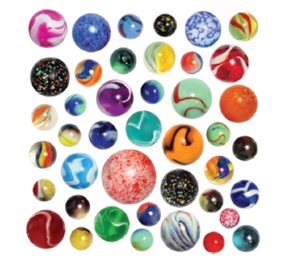
\includegraphics[width=4.89702in,height=6.12128in]{media/image24.png}

\fonte{Prefeitura Municipal de Eunápolis. Vacinação: Covid-19 para crianças de 5 a 11 anos. 
Disponível em: https://www.eunapolis.ba.gov.br/site/Noticias/noticia-060220221925071633-Vacina-o-Covid-19-para-crian-as-de-5-a-11-anos.
Acesso em: 24 mai. 2023.}

A força expressiva da campanha acima advém sobretudo 

\begin{escolha}
    
    \item da imagem inesperada que ilustra o cartaz.
    
    \item do contraste entre as cores de fundo. 
    
    \item do destaque da lista de locais de vacinação. 
    
    \item do jogo de palavras em ``não vacile, vacine''.

\end{escolha}

\coment{SAEB: Identificar o uso de recursos persuasivos em textos verbais e não
verbais

a) Incorreta. A imagem que ilustra o cartaz não é inesperada.
b) Incorreta. O contraste entre as cores de fundo não alcança
grande força expressiva.
c) Incorreta. A lista de locais de vacinação não está em destaque.
d) Correta. O jogo com palavras de sons semelhantes, mas de sentidos
distintos confere força expressiva ao cartaz.}

\num{3} Leia o texto abaixo para responder à questão. 

\begin{quote}

CAPÍTULO I

DISPOSIÇÕES GERAIS

Art. 1º É instituída a Lei Brasileira de Inclusão da Pessoa com
Deficiência (Estatuto da Pessoa com Deficiência), destinada a assegurar
e a promover, em condições de igualdade, o exercício dos direitos e das
liberdades fundamentais por pessoa com deficiência, visando à sua
inclusão social e cidadania.

Parágrafo único. Esta Lei tem como base a Convenção sobre os Direitos
das Pessoas com Deficiência e seu Protocolo Facultativo, ratificados
pelo Congresso Nacional por meio do Decreto Legislativo nº 186, de 9 de
julho de 2008 , em conformidade com o procedimento previsto no § 3º do
art. 5º da Constituição da República Federativa do Brasil , em vigor
para o Brasil, no plano jurídico externo, desde 31 de agosto de 2008, e
promulgados pelo Decreto nº 6.949, de 25 de agosto de 2009 , data de
início de sua vigência no plano interno.

\end{quote}

\fonte{Presidência da República. 
Lei Brasileira de Inclusão da Pessoa com Deficiência (Estatuto da Pessoa com Deficiência).
Disponível em: https://www.planalto.gov.br/ccivil_03/_ato2015-2018/2015/lei/l13146.htm.
Acesso em: 24 mai. 2023.}

O texto acima pertence ao domínio dos textos normativos e tem como
objetivo assegurar os direitos das pessoas com deficiência. Esta
afirmação pode ser comprovada pelo

\begin{escolha}
    
    \item artigo primeiro das disposições gerais.
    
    \item artigo quinto da Constituição Federal.
    
    \item capítulo I.
    
    \item parágrafo único.

\end{escolha}

\coment{SAEB: Identificar formas de organização de textos normativos, 
legais e/ou reivindicatórios.

a) Correta. Logo no primeiro artigo aparecem as disposições gerais e os
temas a serem normalizados pela lei.
b) Incorreta. O artigo quinto da Constituição aparece como reforço e
justificativa da importância da Lei.
c) Incorreta. O capítulo primeiro compreende demais partes e
peculiaridades da Lei.
d) Incorreta. O parágrafo único apresenta as justificativas sobre
pertinência da regulamentação do Estatuto da Pessoa com Deficiência.}

\num{4} Leia o texto abaixo para responder à questão. 

\begin{quote}

Aqui em Manaus faço uma parte desse grande projeto que é desenvolvido
por diversas instituições japonesas e conta com financiamento da GHIT
Funding, tendo à frente o doutor Shigeto Yoshida, da Universidade de
Kanazawa, no Japão, que é o desenvolvedor dessa formulação vacinal.
Essa vacina atua contra o parasita no hospedeiro humano e, também,
tentando evitar a infecção do hospedeiro que é o vetor, que transmite a
doença de uma pessoa para outra. Ela tem na sua forma a proteína CSP,
presente na vacina que já está em uso em diversos países da África e na
vacina desenvolvida pela Universidade de Oxford, no Reino Unido. Então
ela tem esse pedaço do parasita, essa proteína, que é um alvo estudado
já há muitos anos e com poder de proteção para as infecções nos humanos.
Essa proteína tem um papel importante para impedir que o parasita chegue
ao fígado, que é o primeiro local em que ele se instala, e, por causa
disso, os anticorpos e a resposta celular produzidos por uma vacina
poderiam impedir a entrada do parasita e seu desenvolvimento nos
humanos.

\end{quote}

\fonte{Ciça Guedes. Ciência Hoje. Malária: uma vacina contra um desafio amazônico.
Disponível em: https://cienciahoje.org.br/artigo/malaria-uma-vacina-contra-um-desafio-amazonico/
Acesso em: 24 mai. 2023.}

Neste texto, podemos ver a explicação de como devem funcionar as vacinas
contra a malária e como estão sendo desenvolvidas. Assinale a alternativa
cuja expressão destacada seja marcador discursivos de causa.

\begin{escolha}

    \item \ldots ``conta com financiamento da GHIT Funding, \textbf{tendo à frente} o doutor Shigeto Yoshida''.

    \item ``\textbf{e, também}, tentando evitar a infecção do hospedeiro''.

    \item ``\textbf{Então} ela tem esse pedaço do parasita''.

    \item ``e, \textbf{por causa disso}, os anticorpos e a resposta celular''.

\end{escolha}

\coment{SAEB: Identificar elementos constitutivos de gêneros de divulgação científica

a) Incorreta. A expressão destacada expressa a circunstância de modo.
b) Incorreta. A expressão destacada expressa a circunstância de adição.
c) Incorreta. No contexto em que se insere, a expressão destacada é marca de oralidade.
d) Correta. A expressão destacada expressa a circunstância de causa.}

\num{5} Leia os textos abaixo para responder à questão. 

\begin{quote}

\textbf{Exemplo 1}

A relação do ser humano com os animais de estimação existe há mais de 10
mil anos. Os animais domésticos preenchem várias necessidades emocionais
dos homens e dessa forma esses bichinhos, principalmente cães e gatos,
se tornam cada vez mais parte da nossa casa e de nossa família.

Mas infelizmente, muita gente ainda possui animais de estimação, mas não
possui a menor condição de criá-los. E quando falamos em condição de
criar, refiro-me principalmente a condições psicológicas.

Tanto é verdade que os maus-tratos aos ``pets'' são evidentes em todas as
cidades do país: animais famintos, torturados, feridos covardemente,
confinados em espaços minúsculos ou abandonados nas ruas ou estradas
Brasil afora.

E se quisermos mudar essa situação, precisamos perder o medo e o receio
de nos envolver e denunciar os maus-tratos, que só cessarão
quando aqueles que cometem esses crimes começarem a ser exemplarmente
punidos.

\end{quote}

\fonte{Hugo Xavier. Jornal Cidade. Os maus tratos e o abandono de animais. 
Disponível em: https://www.jornalcidademg.com.br/artigo-os-maus-tratos-e-o-abandono-de-animais/. 
Acesso em: 24 mai. 2023.}

\textbf{Exemplo 2}

\begin{quote}

\textbf{Polícia resgata 10 cachorros em situação de maus-tratos em dois
imóveis de Curitiba}

Resgate aconteceu no bairro Abranches e no Barreirinha. Polícia chegou
aos casos após denúncias de vizinhos.

A Polícia Civil e a Rede de Proteção Animal de Curitiba resgataram 10
cachorros que estavam em situação de maus-tratos na capital paranaense,
na quinta-feira (23).

O resgate aconteceu em dois imóveis, um no bairro Abranches e outro no
Barreirinha.

O proprietário do imóvel do Abranches foi multado em R\$ 12 mil, por
criação e venda irregulares e maus-tratos aos animais. A suspeita é que
no local existia um criadouro ilegal.

\end{quote}

\fonte{G1. Polícia resgata 10 cachorros em situação de maus-tratos em dois imóveis de Curitiba.
Disponível em: https://g1.globo.com/pr/parana/noticia/2023/02/24/policia-resgata-10-cachorros-em-situacao-de-maus-tratos-em-dois-imoveis-de-curitiba.ghtml
Acesso em: 24 mai. 2023.}

Os dois exemplos foram extraídos de meios de comunicação e representam
diferentes gêneros do campo jornalístico. Com base nas diferenças entre
os dois textos é correto afirmar que:

\begin{escolha}
    
    \item O Exemplo 1 é uma entrevista e o Exemplo 2 é uma notícia.
    
    \item O Exemplo 1 é um artigo de opinião e o Exemplo 2 uma notícia.
    
    \item O Exemplo 1 é uma reportagem e o Exemplo 2 um artigo de opinião.
    
    \item O Exemplo 1 é uma carta de leitor e o Exemplo 2 é um artigo de opinião.

\end{escolha}

\coment{SAEB: Analisar a relação temática entre diferentes gêneros jornalísticos.

a) Incorreta. O Exemplo 1 é um artigo de opinião; o Exemplo 2, uma notícia.
b) Correta. O Exemplo 1 é artigo de opinião, pois apresenta
argumentação acerca do tema; o Exemplo 2 apresenta claramente estrutura
de notícia, dividido em título, linha fina, lide e corpo, além de 
restringir-se a noticiar o resgate dos animais, sem expressão de 
opinião. 
c) Incorreta. O Exemplo 1 é um artigo de opinião; o Exemplo 2, uma notícia.
d) Incorreta. O Exemplo 1 é um artigo de opinião; o Exemplo 2, uma notícia.}

\num{6} Leia o soneto abaixo para responder à questão. 

\begin{quote}
\begin{verse}

Apartava-se Nise de Montano, \\
em cuja alma partindo se ficava; \\
que o pastor na memória a debuxava, \\
por poder sustentar-se deste engano.

Pelas praias do Índico Oceano \\
sobre o curvo cajado se encostava, \\
e os olhos pelas águas alongava, \\
que pouco se doíam de seu dano.

Pois com tamanha mágoa e saudade \\
(dizia) quis deixar me a que eu adoro, \\
por testemunhas tomo Céu e estrelas.

Mas se em vós, ondas, mora piedade, \\
levai também as lágrimas que choro, \\
pois assim me levais a causa delas!

\end{verse}
\end{quote}

\fonte{Luís de Camões. Sonetos.  
Disponível em: http://www.dominiopublico.gov.br/download/texto/bv000164.pdf.
Acesso em: 24 mai. 2023.}

Considerando os elementos que caracterizam os textos literários, o texto
acima pode ser considerado

\begin{escolha}

    \item conto, com personagens de ações restritas a espaço limitado.
    
    \item texto dramático, com falas de personagens e rubricas.  
    
    \item poema, baseado na sonoridade de versos divididos em estrofes.  
    
    \item romance, extensa narração de ações de diversos conflitos. 

\end{escolha}

\coment{SAEB: Analisar elementos constitutivos de textos pertencentes ao domínio
literário.

a) Incorreta. O texto é um poema.
b) Incorreta. O texto é um poema.
c) Correta. O texto é um soneto, forma poemática de quatro estrofes, 
dois quartetos e dois tercetos, cujos versos rimados e metrificados 
imprimem sonoridade regular ao conjunto. 
d) Incorreta. O texto é um poema.}

\num{7} Leia o texto abaixo para responder à questão. 

\begin{quote}

\textbf{Falta de iluminação em rua completa 1 ano e tem ``festa de
aniversário'' como protesto em Ourinhos}

Manifestação foi na Rua Narciso Nicolosi, no Jardim Paulista. Prefeitura
informou na manhã seguinte ao ato que fez a troca de lâmpada queimada.

Moradores de Ourinhos (SP) protestaram contra a falta de iluminação
pública na Rua Narciso Nicolosi, no Jardim Paulista, na noite desta
quarta-feira (26) com uma ``festa de aniversário'' para marcar um ano de
espera pela troca de lâmpadas em um poste.

A ``comemoração'' teve bolo com vela, refrigerante, bexigas, cartazes e
parabéns para você em coro e palmas em meio a críticas pela escuridão.

\end{quote}

\fonte{G1. Falta de iluminação em rua completa 1 ano e tem 'festa de 
aniversário' como protesto em Ourinhos. 
Disponível em: https://g1.globo.com/sp/bauru-marilia/noticia/2023/04/27/falta-de-iluminacao-em-rua-completa-1-ano-e-tem-festa-de-aniversario-como-protesto-em-ourinhos.ghtml.
Acesso em: 24 mai. 2023.}

Os termos entre aspas na notícia expressam

\begin{escolha}
    
    \item ironia. 
    
    \item citação de falas de autoridades da cidade.
    
    \item citação de argumentos de especialistas.
    
    \item enfase nas palavras e termos destacados.

\end{escolha}

\coment{SAEB: Analisar efeitos de sentido produzido pelo uso de formas
de apropriação textual (paráfrase, citação etc.).

a) Correta. Os termos estão sendo usados de forma irônica para protestar
contra a falta de energia.
b) Incorreta. O uso de aspas neste caso não indica a fala de
autoridades.
c) Incorreta. O uso das aspas neste caso não introduz falas
de especialistas.
d) Incorreta. Os termos não estão sendo puramente enfatizados, o uso de
aspas se dá principalmente pelo contexto irônico da notícia.}

\num{8} Leia o texto abaixo para responder à questão. 

\begin{quote}

\textbf{Telegram diz que Justiça ordenou entrega de dados ``impossíveis''
de serem obtidos; PF afirma que lentidão permitiu exclusão de
informações}

\textit{Cofundador do aplicativo afirmou que empresa está recorrendo da
suspensão do serviço, que começou a valer na noite da última quarta
(26).}

O cofundador do Telegram Pavel Durov afirmou nesta quinta-feira (27) que
a Justiça brasileira ordenou a entrega de dados ``impossíveis'' de serem
coletados. Em seu canal no aplicativo, ele afirmou que a empresa vai
recorrer da decisão.

\end{quote}

\fonte{G1. Telegram diz que Justiça ordenou entrega de dados impossíveis 
de serem obtidos; PF afirma que lentidão permitiu exclusão de informações. 
Disponível em: https://g1.globo.com/tecnologia/noticia/2023/04/27/telegram-diz-que-justica-ordenou-coleta-de-dados-impossiveis-de-serem-obtidos-pf-afirma-que-lentidao-permitiu-exclusao-de-informacoes.ghtml.
Acesso em: 24 mai. 2023.}

Considerando a notícia acima, pode-se afirmar que o título da notícia expressa

\begin{escolha}

    \item concordância do autor com a justificativa da empresa. 

    \item simpatia do autor pela decisão da Polícia Federal.  

    \item intenção de influenciar a opinião do leitor.  

    \item tentativa de apresentar dois pontos de vista opostos. 

\end{escolha}

\coment{SAEB: Analisar os efeitos de sentido decorrentes dos mecanismos de 
construção de textos jornalísticos/midiáticos.

a) Incorreta. O título não contém concordância do autor com a justificativa da empresa.
b) Incorreta. O título não contém simpatia do autor pela decisão da Polícia Federal.
c) Incorreta. Não há elementos que permitam afirma que o autor tenha tentado
influenciar a opinião do leitor.
d) Correta. A extensão do título da notícia já revela a intenção do autor: 
apresentar dois pontos de vista opostos (o do Telegram e o da Polícia Federal),
separados por ponto e vírgula.}

\num{9} Leia o texto abaixo para responder à questão. 

\begin{quote}

\textbf{O rato do mato e o rato da cidade}

Um ratinho da cidade foi uma vez convidado para ir à casa
de um rato do campo. Vendo que seu companheiro vivia pobremente de
raízes e ervas, o rato da cidade convidou-o a ir morar com ele:

-- Tenho muita pena da pobreza em que você vive --
disse. -- Venha morar comigo na cidade e você verá como lá a
vida é mais fácil.

Lá se foram os dois para a cidade, onde se acomodaram
numa casa rica e bonita.

Foram logo à despensa e estavam muito bem, se
empanturrando de comidas fartas e gostosas, quando entrou uma
pessoa com dois gatos, que pareceram enormes ao ratinho do
campo.

Os dois ratos correram espavoridos para se esconder.

-- Eu vou para o meu campo -- disse o rato do campo
quando o perigo passou. -- Prefiro minhas raízes e ervas na
calma, às suas comidas gostosas com todo esse susto.

\textit{Mais vale magro no mato que gordo na boca do gato.} 

\end{quote}

\fonte{Ana Rosa Abreu e outros autores. Alfabetização: livro do aluno. Vol.2: 
contos tradicionais, fábulas, lendas e mitos. Disponível em: 
http://www.dominiopublico.gov.br/download/texto/me001614.pdf.
Acesso em: 24 mai. 2023.}

A frase final, destacada em itálico, tem a finalidade de 

\begin{escolha}
    
    \item adicionar elementos à fábula, explicando-lhe o sentido. 
    
    \item resumir de forma expressiva o sentido da fábula. 
    
    \item propor ao leitor uma pergunta sobre o sentido da fábula.
    
    \item remeter a conclusão da fábula a um outro texto.  

\end{escolha}

\coment{SAEB: Inferir informações implícitas em distintos textos

a) Correta. O trecho final, em destaque, chama-se \textit{moral da história}
e serve para sintetizar, de maneira expressiva (observe-se a rima entre
\textit{mato} e \textit{gato}) o sentido da fábula. 
b) Incorreta. A moral da história resume de forma expressiva o sentido da 
fábula.
c) Incorreta. A moral da história resume de forma expressiva o sentido da 
fábula.
d) Incorreta. A moral da história resume de forma expressiva o sentido da 
fábula.}

\num{10} Leia o texto abaixo para responder à questão. 

\begin{quote}

Os recifes de coral são ambientes extremamente diversos, abrigando cerca
de 25\% de toda a biodiversidade marinha. Suas estruturas rígidas são
constituídas por organismos marinhos de esqueleto calcário, os corais.
Mas há outros tipos de organismos que vivem nos recifes, como algas,
moluscos e peixes.

Além de sua importância biológica, recifes também são valiosos do ponto
de vista socioeconômico. A elevada biodiversidade produz bastante
pescado, de modo que, hoje, cerca de 10\% da proteína animal consumida
no planeta provem de recifes de coral. Outro fator a considerar é que a
beleza natural estimula o turismo, e, consequentemente, o
estabelecimento de operadoras de mergulho, pousadas e restaurantes.

\end{quote}

\fonte{Tássia Biazon. Ciência Hoje. Recifes sob estresse. 
Disponível em: https://cienciahoje.org.br/artigo/recifes-sob-estresse/. 
Acesso em: 24 mai. 2023. com adaptações.}

A importância biológica dos recifes de coral pode ser comprovada por:

\begin{escolha}
    
    \item conterem beleza natural que estimula o turismo e o comércio de
  pousadas e restaurantes.
    
    \item serem estruturas rígidas constituídas por organismos marinhos de
  esqueleto calcário, chamadas de corais.
    
    \item serem ambientes extremamente diversos, abrigando cerca de 25\% de
  toda a biodiversidade marinha.
    
    \item contribuírem com a presença de peixes favorecendo a produção de
  pescado.

\end{escolha}

\coment{SAEB: Distinguir fatos de opiniões em textos.

a) Incorreta. O turismo e o comércio não se referem à importância 
\textit{biológica} dos recifes de coral: essas atividades dizem respeito a
seu valor socioeconômico.
b) Incorreta. A alternativa contém a descrição objetiva da estrutura dos
corais, não sua importância biológica.
c) Correta. Segundo o texto, os recifes de corais são importantes
biologicamente por abrigarem grande biodiversidade.
d) Incorreta. A produção de pescado não se refere à importância 
\textit{biológica} dos recifes de coral: essa atividade diz respeito
a seu valor socioeconômico.}

\num{11} Leia o texto abaixo para responder à questão. 

\begin{quote}

Algumas atitudes da sociedade têm colaborado para que as crianças
desenvolvam hábitos alimentares saudáveis. É o caso de escolas que
procuram controlar o tipo de comida consumida pelos seus alunos. Na
cantina ou lancheira são proibidos doces e frituras. Caso a criança os
traga de casa, esses alimentos são mandados de volta e uma outra solução
é dada para a refeição daquele dia.

Mesmo assim, alguns pais acabam infringindo as regras e mandando como
lanche para seus filhos alguns alimentos proibidos. Muitos justificam
que, se não for aquilo, a criança não come, sendo melhor que coma algo
sem qualidade que ficar de estômago vazio.

\end{quote}

\fonte{Ana Cássia Maturano. G1. Alimentação saudável na mira das escolas e dos pais.
Disponível em: https://g1.globo.com/educacao/noticia/2010/04/opiniao-alimentacao-saudavel-na-mira-das-escolas-e-dos-pais.html.
Acesso em: 24 mai. 2023.}

No último parágrafo do texto o autor deixa claro que

\begin{escolha}
    
    \item as escolas não se empenham em promover uma alimentação saudável para os
  estudantes.
    
    \item os pais se empenham em promover uma alimentação saudável para os
  filhos.
    
    \item pais e escolas estão empenhados em oferecer uma alimentação saudável para
  os estudantes.
    
    \item alguns pais não se empenham em oferecer uma alimentação saudável para os filhos.

\end{escolha}

\coment{SAEB: Analisar os processos de referenciação lexical e pronominal.

a) Incorreta. No último parágrafo, a autora afirma que, apesar das restrições
e atitudes de algumas escolas, há pais que não se empenham em oferecer uma alimentação saudável para os filhos.
b) Incorreta. No último parágrafo, a autora afirma que, apesar das restrições
e atitudes de algumas escolas, há pais que não se empenham em oferecer uma alimentação saudável para os filhos.
c) Incorreta. No último parágrafo, a autora afirma que, apesar das restrições
e atitudes de algumas escolas, há pais que não se empenham em oferecer uma alimentação saudável para os filhos.
d) Correta. No último parágrafo, a autora afirma que, apesar das restrições
e atitudes de algumas escolas, há pais que não se empenham em oferecer uma alimentação saudável para os filhos.}

\num{12} Leia o texto abaixo para responder à questão. 

\begin{quote}

\textbf{Direito da criança de brincar na rua é negligenciado}

\emph{Carimba, cabra-cega, passa anel, boca-de forno, batata-quente:
crianças desconhecem muitas brincadeiras}

Simplesmente brincar. Na rua, nas praças, quadras, parquinho, com
amigos, com vizinhos. É direito constitucional, está nos estatutos,
declarações e lei. Mas, efetivamente, a brincadeira está bem longe de
ser uma prioridade, tanto para muitas crianças, quanto para os pais.

\end{quote}

\fonte{Diário do Nordeste. Direito da criança de brincar na rua é 
negligenciado. Disponível em: https://diariodonordeste.verdesmares.com.br/metro/direito-da-crianca-de-brincar-na-rua-e-negligenciado-1.621061.
Acesso em: 24 mai. 2023.}

A leitura atenta da reportagem permite afirmar que há marca de parcialidade
no trecho:

\begin{escolha}
  
    \item Simplesmente brincar.
  
    \item Direito da criança de brincar na rua é negligenciado.
  
    \item Na rua, nas praças, quadras, parquinho, com amigos, com vizinhos.
  
    \item É direito constitucional, está nos estatutos, declarações e lei.

\end{escolha}

\coment{SAEB: Avaliar diferentes graus de parcialidade em textos jornalísticos.

a) Incorreta. O trecho não apresenta parcialidade.
b) Correta. A opinião expressa no título da notícia está evidente 
no uso do adjetivo \textit{negligenciado}.
c) Incorreta. O trecho não apresenta parcialidade.
d) Incorreta. O trecho não apresenta parcialidade.}

\num{13} Leia o texto abaixo para responder à questão. 

\begin{quote}

\textbf{Strava mostra aumento do número de ciclistas, pós pandemia, em
seis capitais}

A pandemia trouxe algumas mudanças positivas que têm tudo para se tornar
permanentes para muitas pessoas. Uma delas foi o maior número de
ciclistas pelas cidades, que começaram a utilizar o meio de locomoção
com o receio de compartilhar viagens em carros e transportes urbanos.

\end{quote}

\fonte{Daniel Ottoni. Strava mostra aumento do número de ciclistas, pós pandemia, em seis capitais. 
Disponível em: https://www.otempo.com.br/opiniao/esportivamente/strava-mostra-aumento-do-numero-de-ciclistas-pos-pandemia-em-seis-capitais-1.2571161.
Acesso em: 24 mai. 2023.}

Na primeira parte do texto o uso da expressão ``têm tudo para se
tornar'' representa:

\begin{escolha}

    \item otimismo do autor em relação manuntenção das mudanças positivas
  impostas pela pandemia.

    \item pessimismo do autor em relação à continuidade das atitudes
  positivas impulsionadas pela pandemia.

    \item posição neutra em relação às mudanças positivas que chegaram com a
  pandemia.

    \item condição para que as mudanças positivas impostas pela pandemia se
  perpetuem.

\end{escolha}

\coment{SAEB: Identificar os recursos de modalização em textos diversos.

a) Correta. O autor expressa otimismo por meio desse recurso de modalização.
b) Incorreta. A expressão o uso da expressão ``têm tudo para se
tornar'' expressa otimismo.
c) Incorreta.  Incorreta. A expressão o uso da expressão ``têm tudo para se
tornar'' expressa otimismo.
d) Incorreta. Incorreta. A expressão o uso da expressão ``têm tudo para se
tornar'' expressa otimismo.}

\num{14} Leia o texto abaixo para responder à questão. 

\begin{quote}

A Academia Americana de Medicina do Sono recomenda que crianças e
adolescentes entre 6 e 12 anos durmam ao menos nove horas por dia, mas
muitos não seguem a recomendação e os pesquisadores queriam entender
melhor o impacto de menos horas de descanso no desenvolvimento desses
jovens.

Os cientistas analisaram os dados de 8.323 crianças de 9 e 10 anos. Eles
dividiram esse conjunto em dois grupos das crianças que dormiam menos de
nove horas (4.181 participantes) e daquelas que dormiam pelo menos nove
horas (4.142 participantes) -- e avaliaram seus dados neurais e
comportamentais no início da pesquisa e após dois anos.

Os cientistas notaram também uma diferença significativa no volume de
massa cinzenta em 12 das 184 regiões avaliadas, padrão que se repetiu
depois de dois anos, sugerindo que algumas medidas estruturais são
suscetíveis a períodos insuficientes de sono.

\end{quote}

\fonte{O Tempo. Dormir menos de nove horas afeta cérebro e comportamento das crianças.
Disponível em:
https://www.otempo.com.br/mundo/dormir-menos-de-nove-horas-afeta-cerebro-e-comportamento-das-criancas-1.2707918
Acesso em: 24 mai. 2023.}

No texto acima a principal estratégia de argumentação se dá por meio de:

\begin{escolha}

    \item falas de especialistas e opiniões de pais.

    \item discurso de autoridade.

    \item exemplos históricos.

    \item dados de pesquisas.

\end{escolha}

\coment{SAEB: Avaliar a eficácia das estratégias argumentativas em textos de
diferentes gêneros.

a) Incorreta. O texto não contém falas de especialistas nem opinião de pais.
b) Incorreta. Não há citação de discursos de autoridade no texto.
c) Incorreta. Não há exemplos históricos no texto.
d) Correta. O texto se apoia em dados de pesquisas.}

\num{15} Leia o texto abaixo para responder à questão. 

%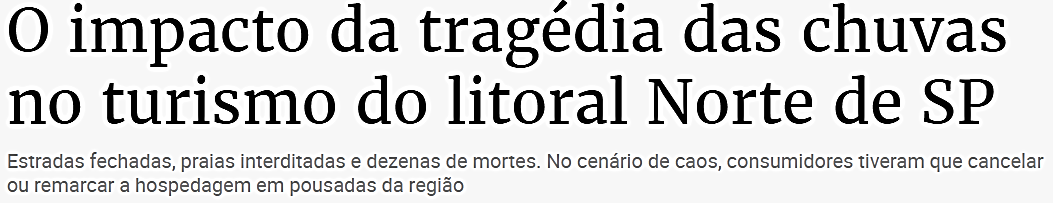
\includegraphics[width=2.84494in,height=2.84494in]{media/image6.png}

\begin{quote}

Desgostoso com a existência medíocre na sua pequena cidade natal, 
um belo dia, aí pelos seus vinte e dois anos, aceitara o convite de um
engenheiro inglês que, por aquelas bandas, andava a explorar
terras e terrenos diamantíferos. Todos julgavam que o ``seu'' mister 
andasse fazendo isso; a verdade, porém, é que o sábio inglês fazia estudos
desinteressados. Fazia puras e platônicas pesquisas geológicas e mineralógicas.
O diamante não era o fim dos seus trabalhos; mas o povo, que teimava em ver,
pelos arredores da cidade, o ventre da terra cheio de diamantes, não podia 
supor que um inglês que levava a catar pedras, pela manhã e até à noite,
tomando notas e com uns instrumentos rebarbativos, não estivesse com tais 
gatimonhas a caçar diamantes. Não havia meio do mister convencer à simplória 
gente do lugar que ele não queria saber de diamantes. 

\end{quote}

\fonte{Lima Barreto. Clara dos Anjos. 
Disponível em: http://www.dominiopublico.gov.br/download/texto/bn000048.pdf.
Acesso em: 25 mai. 2023.}

Levando em consideração o conjunto do parágrafo, a expressão que melhor 
sintetiza o respeito do povo para com o estrangeiro sonhador é

\begin{escolha}

    \item engenheiro inglês.

    \item ``seu'' mister.

    \item o sábio inglês. 

    \item um inglês que levava a catar pedras

\end{escolha}

\coment{SAEB: Avaliar a adequação das variedades linguísticas em contextos de uso.

a) Incorreta. A expressão ``engenheiro inglês'' é usada pelo narrador para
referir-se ao estrangeiro, não pela população local.
b) Correta. A expressão \textit{``seu'' mister} é usada pela população local
para referir-se ao estrangeiro. O uso de ``seu'' já manifesta o respeito 
a ele, que era considerado um sábio. 
c) Incorreta. A expressão ``o sábio inglês'' é usada pelo narrador para
referir-se ao estrangeiro, não pela população local.
d) Incorreta. A expressão ``um inglês que levava a catar pedras'', meramente
descritiva, é usada pelo narrador para referir-se ao estrangeiro e não expressa
o respeito da população a ele.}
